% !TEX root = ../G-design.tex
\subsection{投稿者}
\subsubsection{新規投稿機能}
本機能は、投稿者がスマートフォンの操作方法や活用方法に関する情報を新規投稿する機能である。投稿者は、自力で投稿機能とAI支援機能の二種類を選択し投稿を行える。それぞれは別の機能として説明を行う。それぞれの機能の入力が完了すると投稿画面が表示され再編集や投稿を完了させることができる。
\begin{figure}[H]
    \centering
    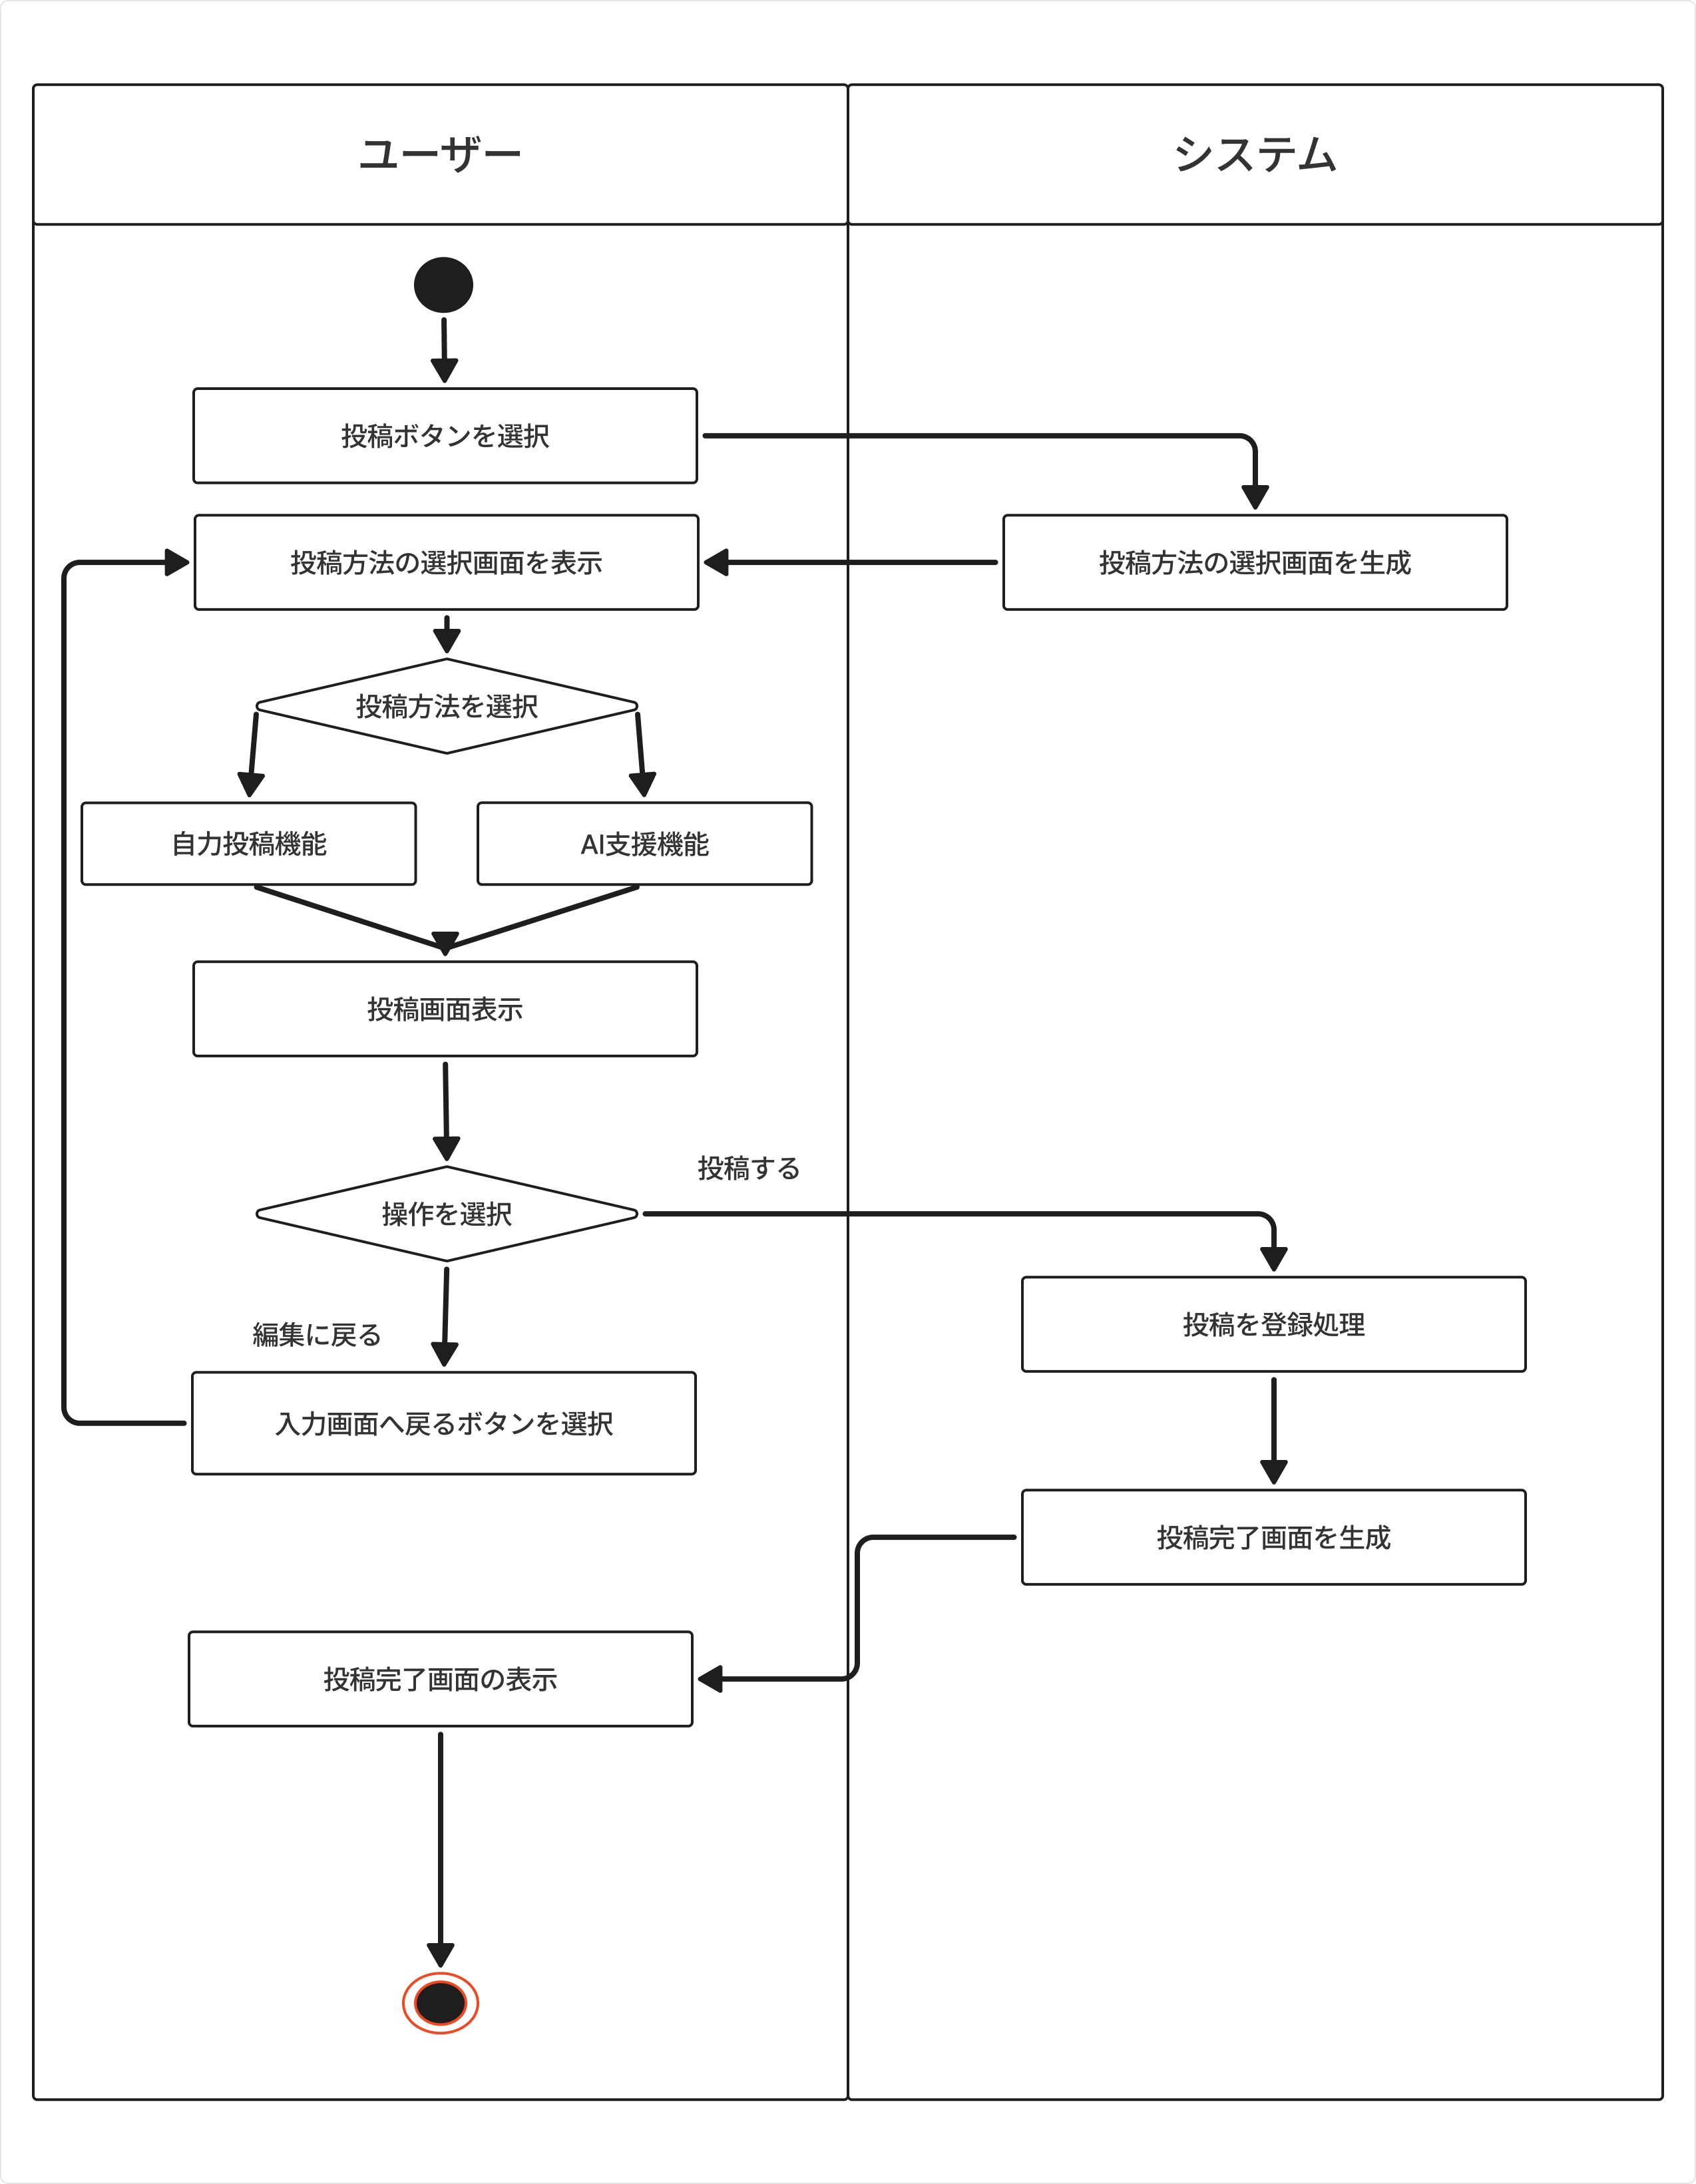
\includegraphics[width=0.5\textwidth]{chapters/images/a.png}
    \caption{新規投稿機能}
\end{figure}
\subsubsection{AI支援機能}
新規投稿機能のAI支援機能の説明である。
本機能は、新規投稿をAIを利用し解決を行う支援機能である。フォームにメモとして入力し、AIで投稿文を生成し投稿者の負担を軽減する。
\begin{figure}[H]
    \centering
    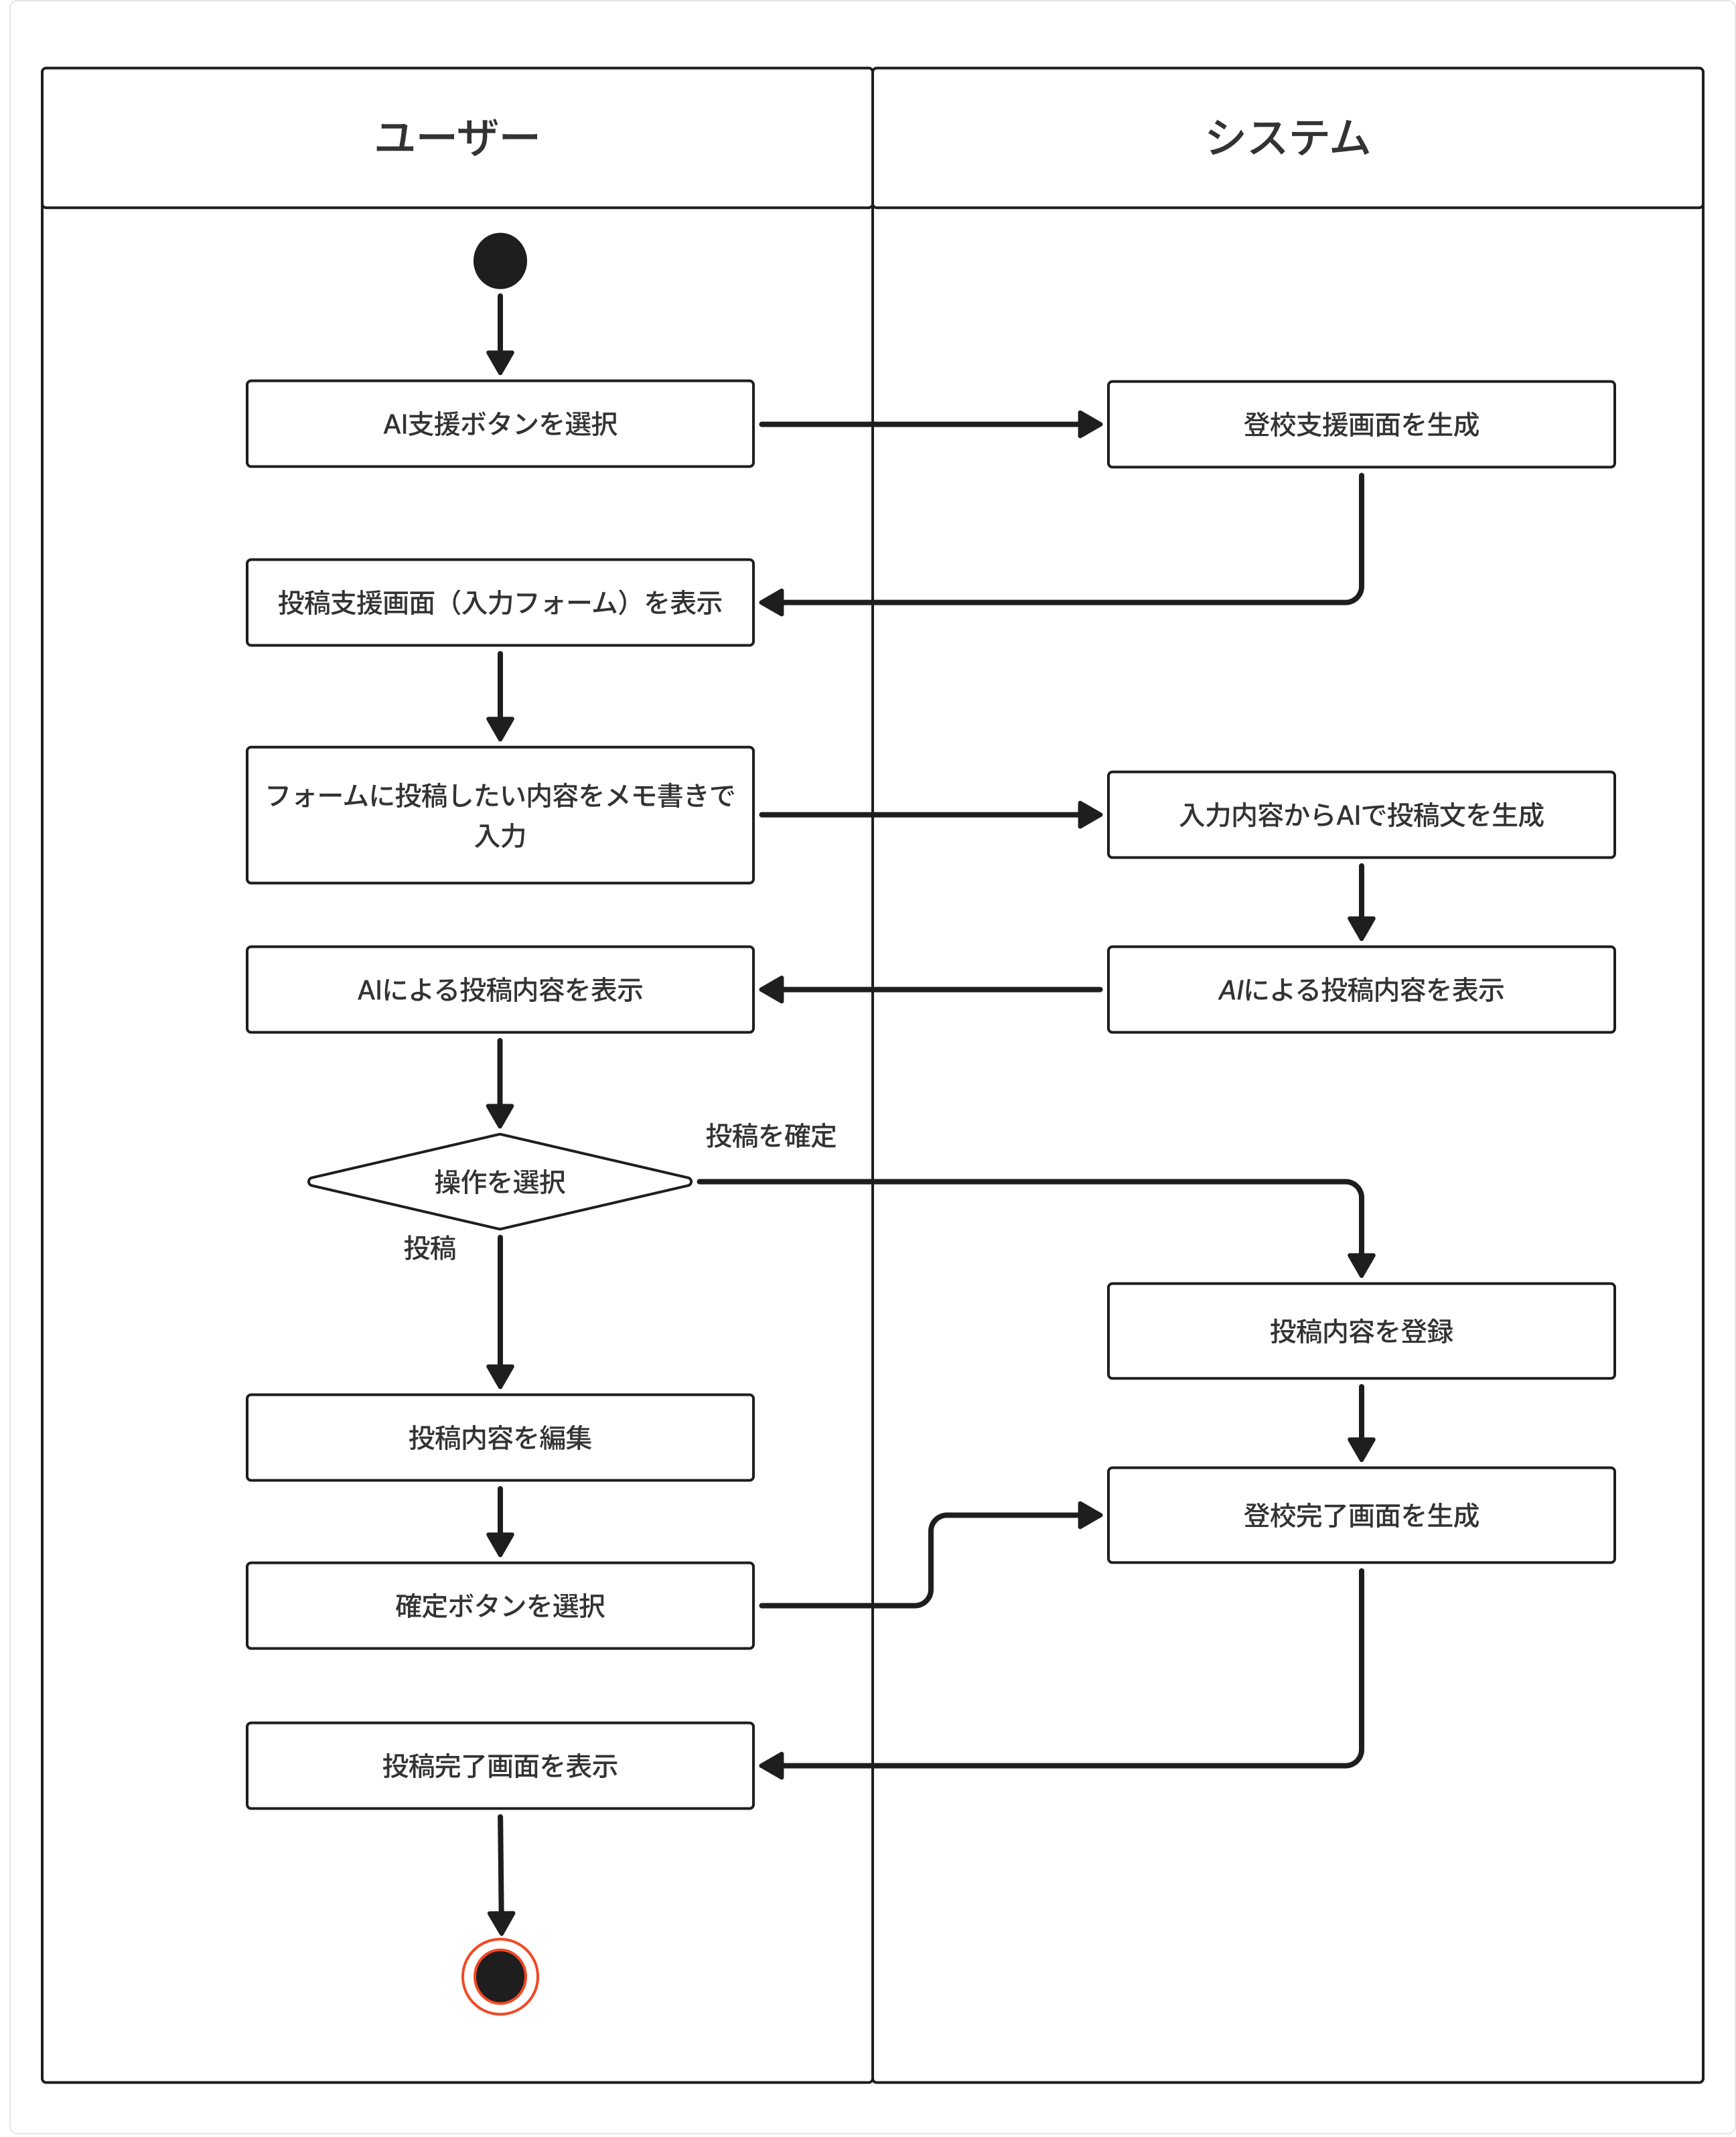
\includegraphics[width=0.5\textwidth]{chapters/images/b.png}
    \caption{AI支援機能}
\end{figure}

\subsubsection{自力投稿機能}
新規投稿機能の自力投稿機能の説明である。
本機能は、新規投稿を自分の言葉で生成し解決する機能である。投稿内容でわかり易く書ける人や有識者の説明が届く仕組みである。
\begin{figure}[H]
    \centering
    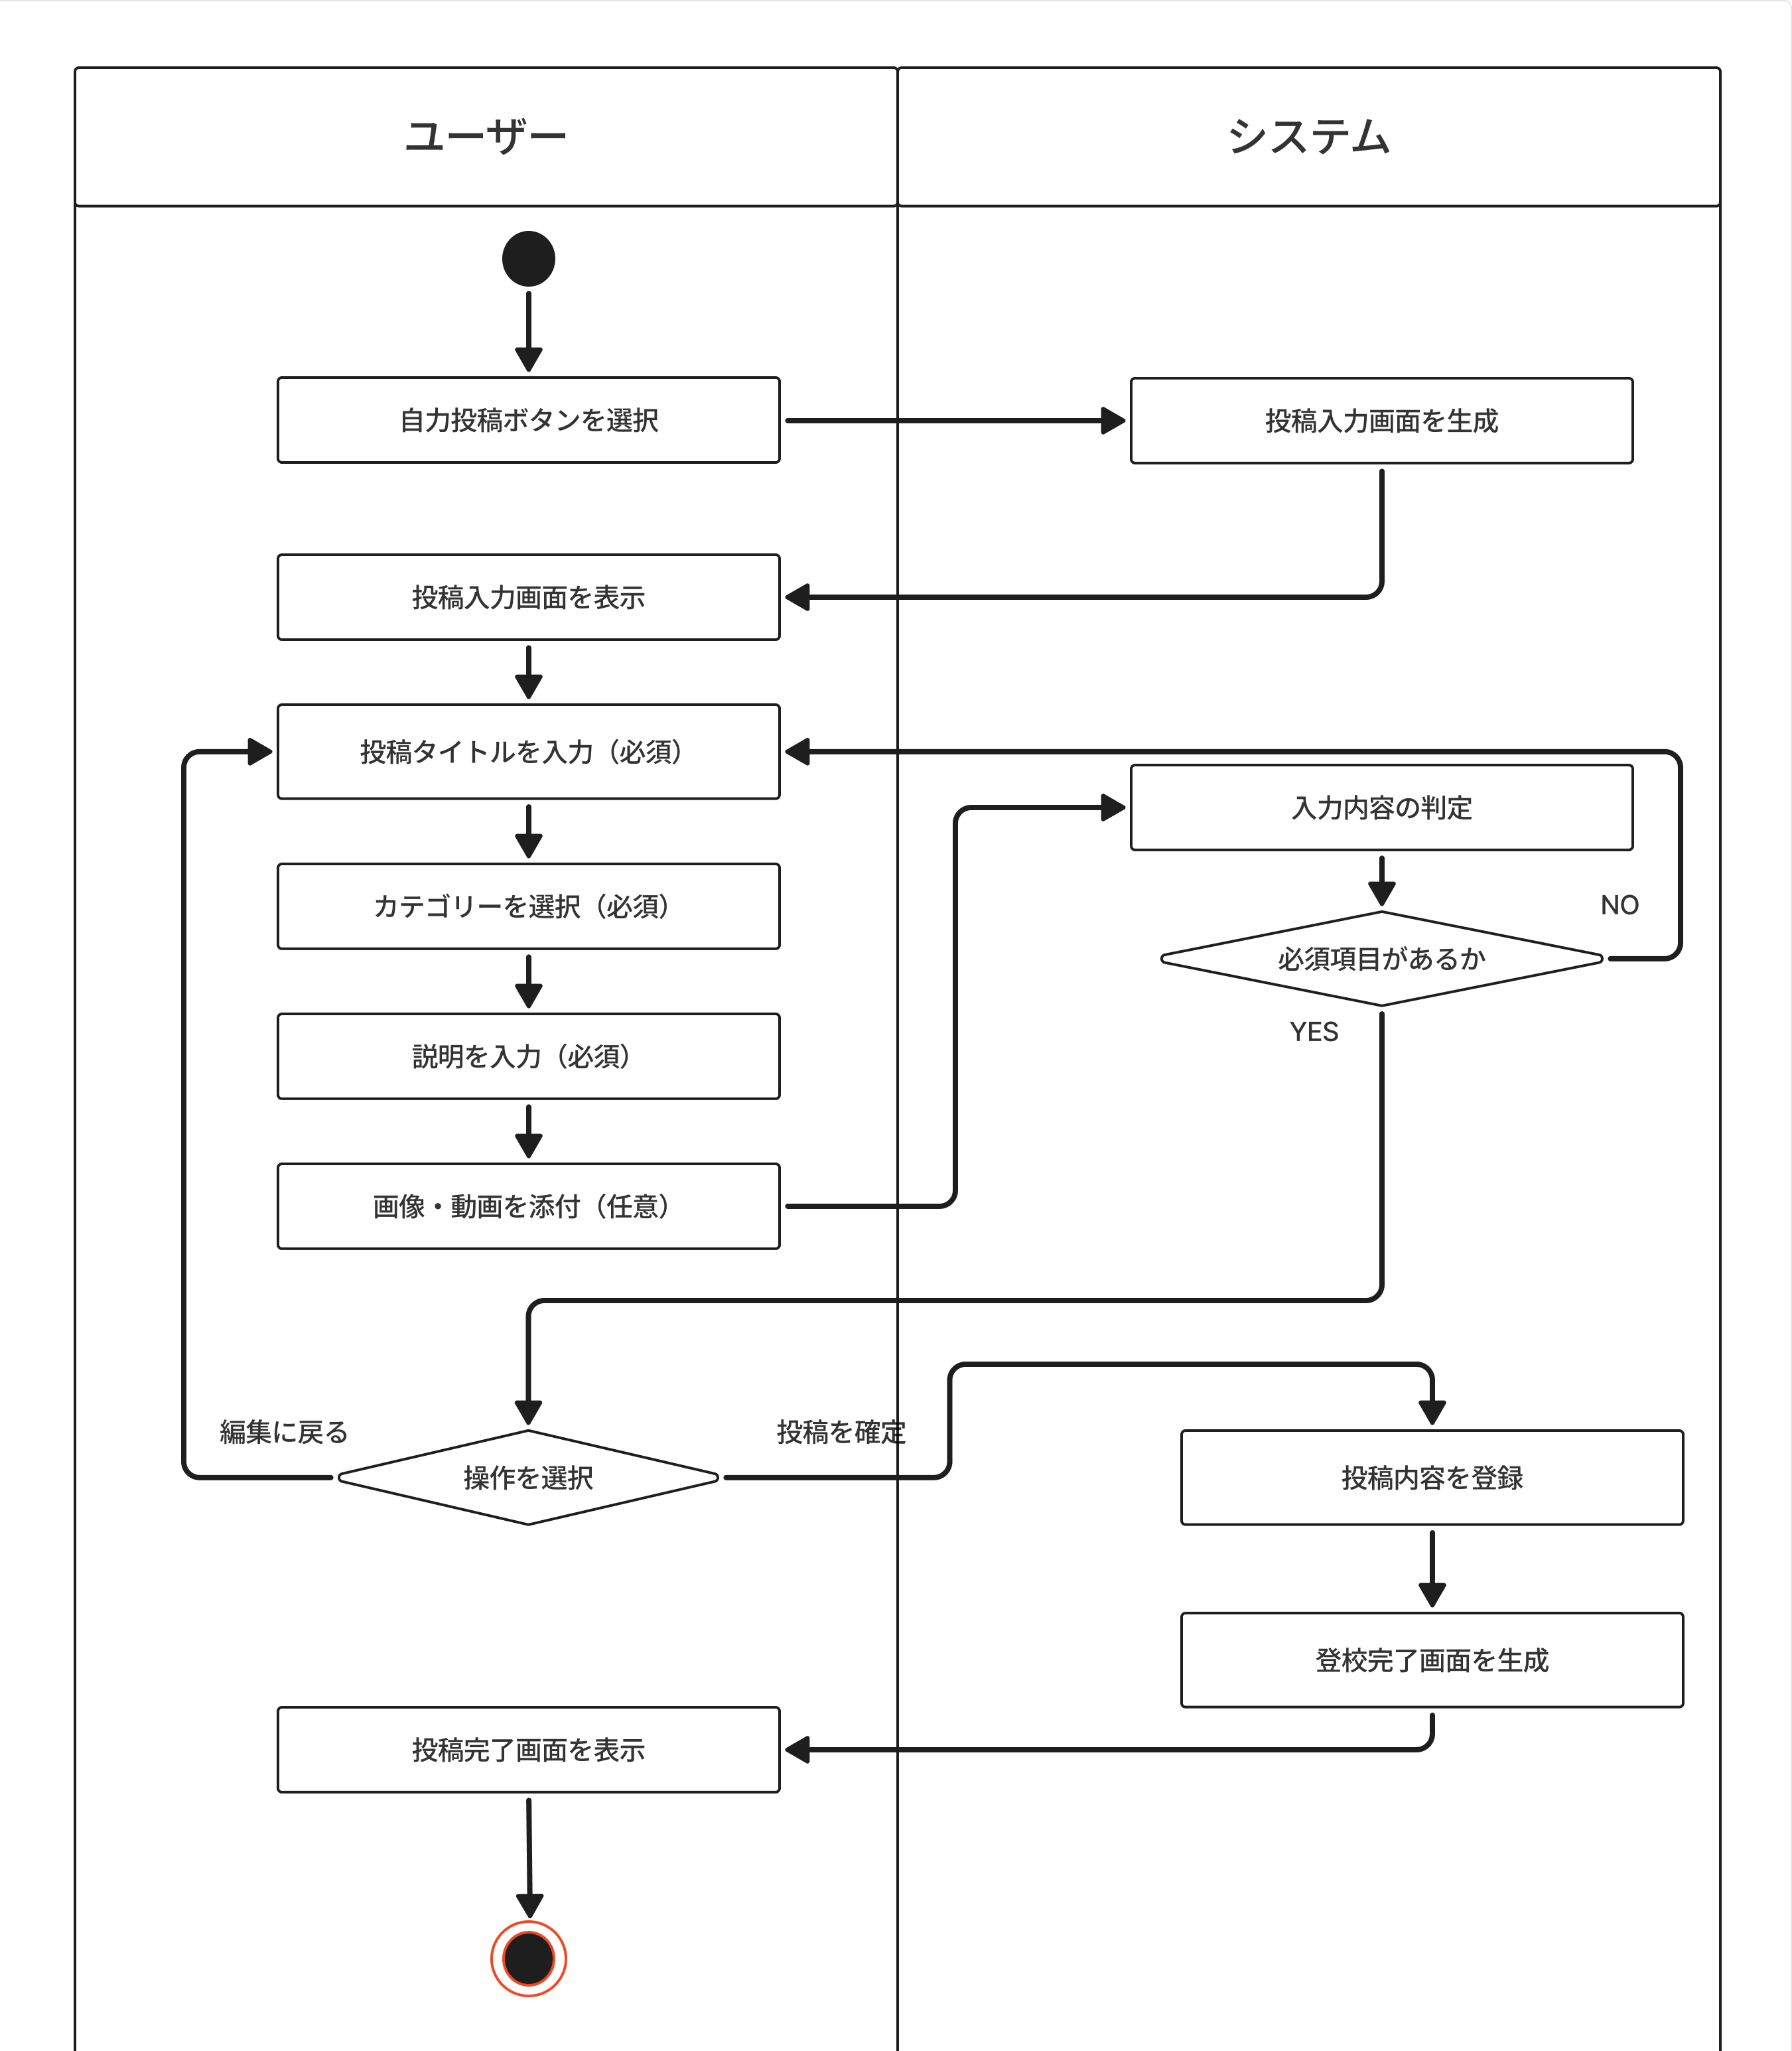
\includegraphics[width=0.5\textwidth]{chapters/images/c.png}
    \caption{自力投稿機能}
\end{figure}
\subsubsection{投稿一覧機能}
本機能は、投稿者自身の投稿を一覧を閲覧・詳細に飛ぶことができる。
\begin{figure}[H]
    \centering
    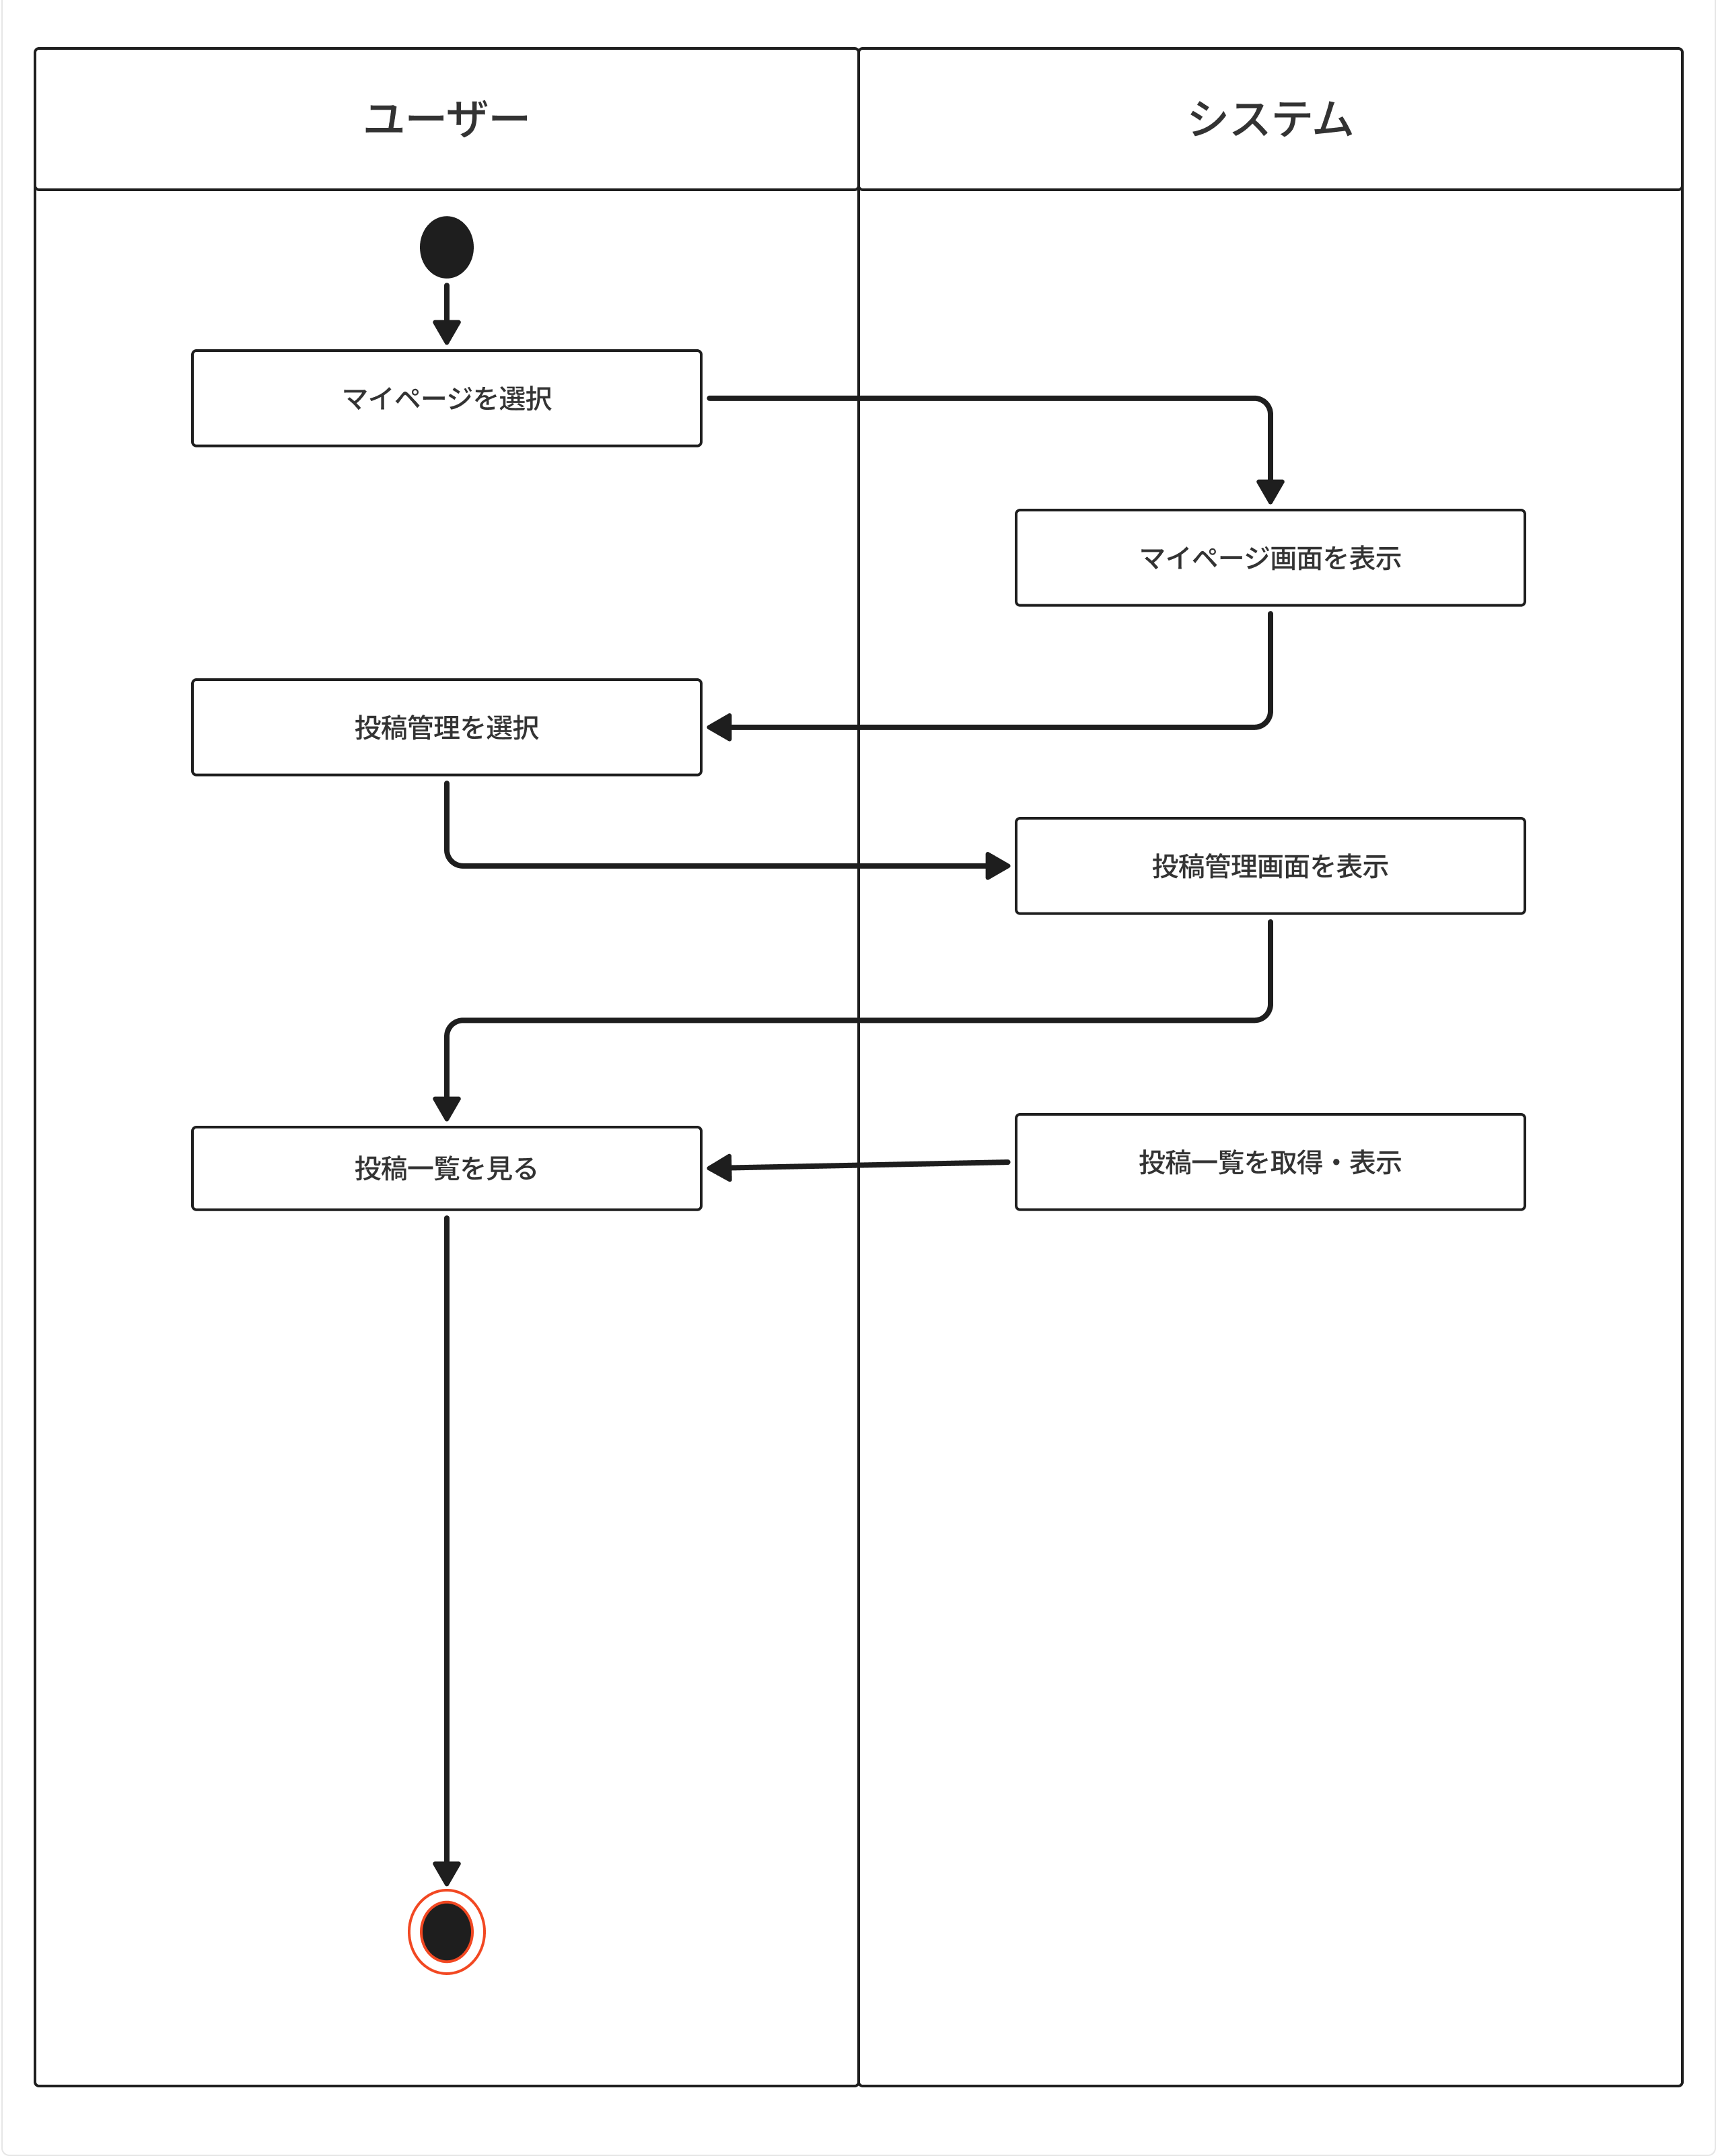
\includegraphics[width=0.5\textwidth]{chapters/images/d.png}
    \caption{投稿一覧機能}
\end{figure}
\subsubsection{投稿削除機能}
本機能は、投稿の一覧から投稿を削除できる。
\begin{figure}[H]
    \centering
    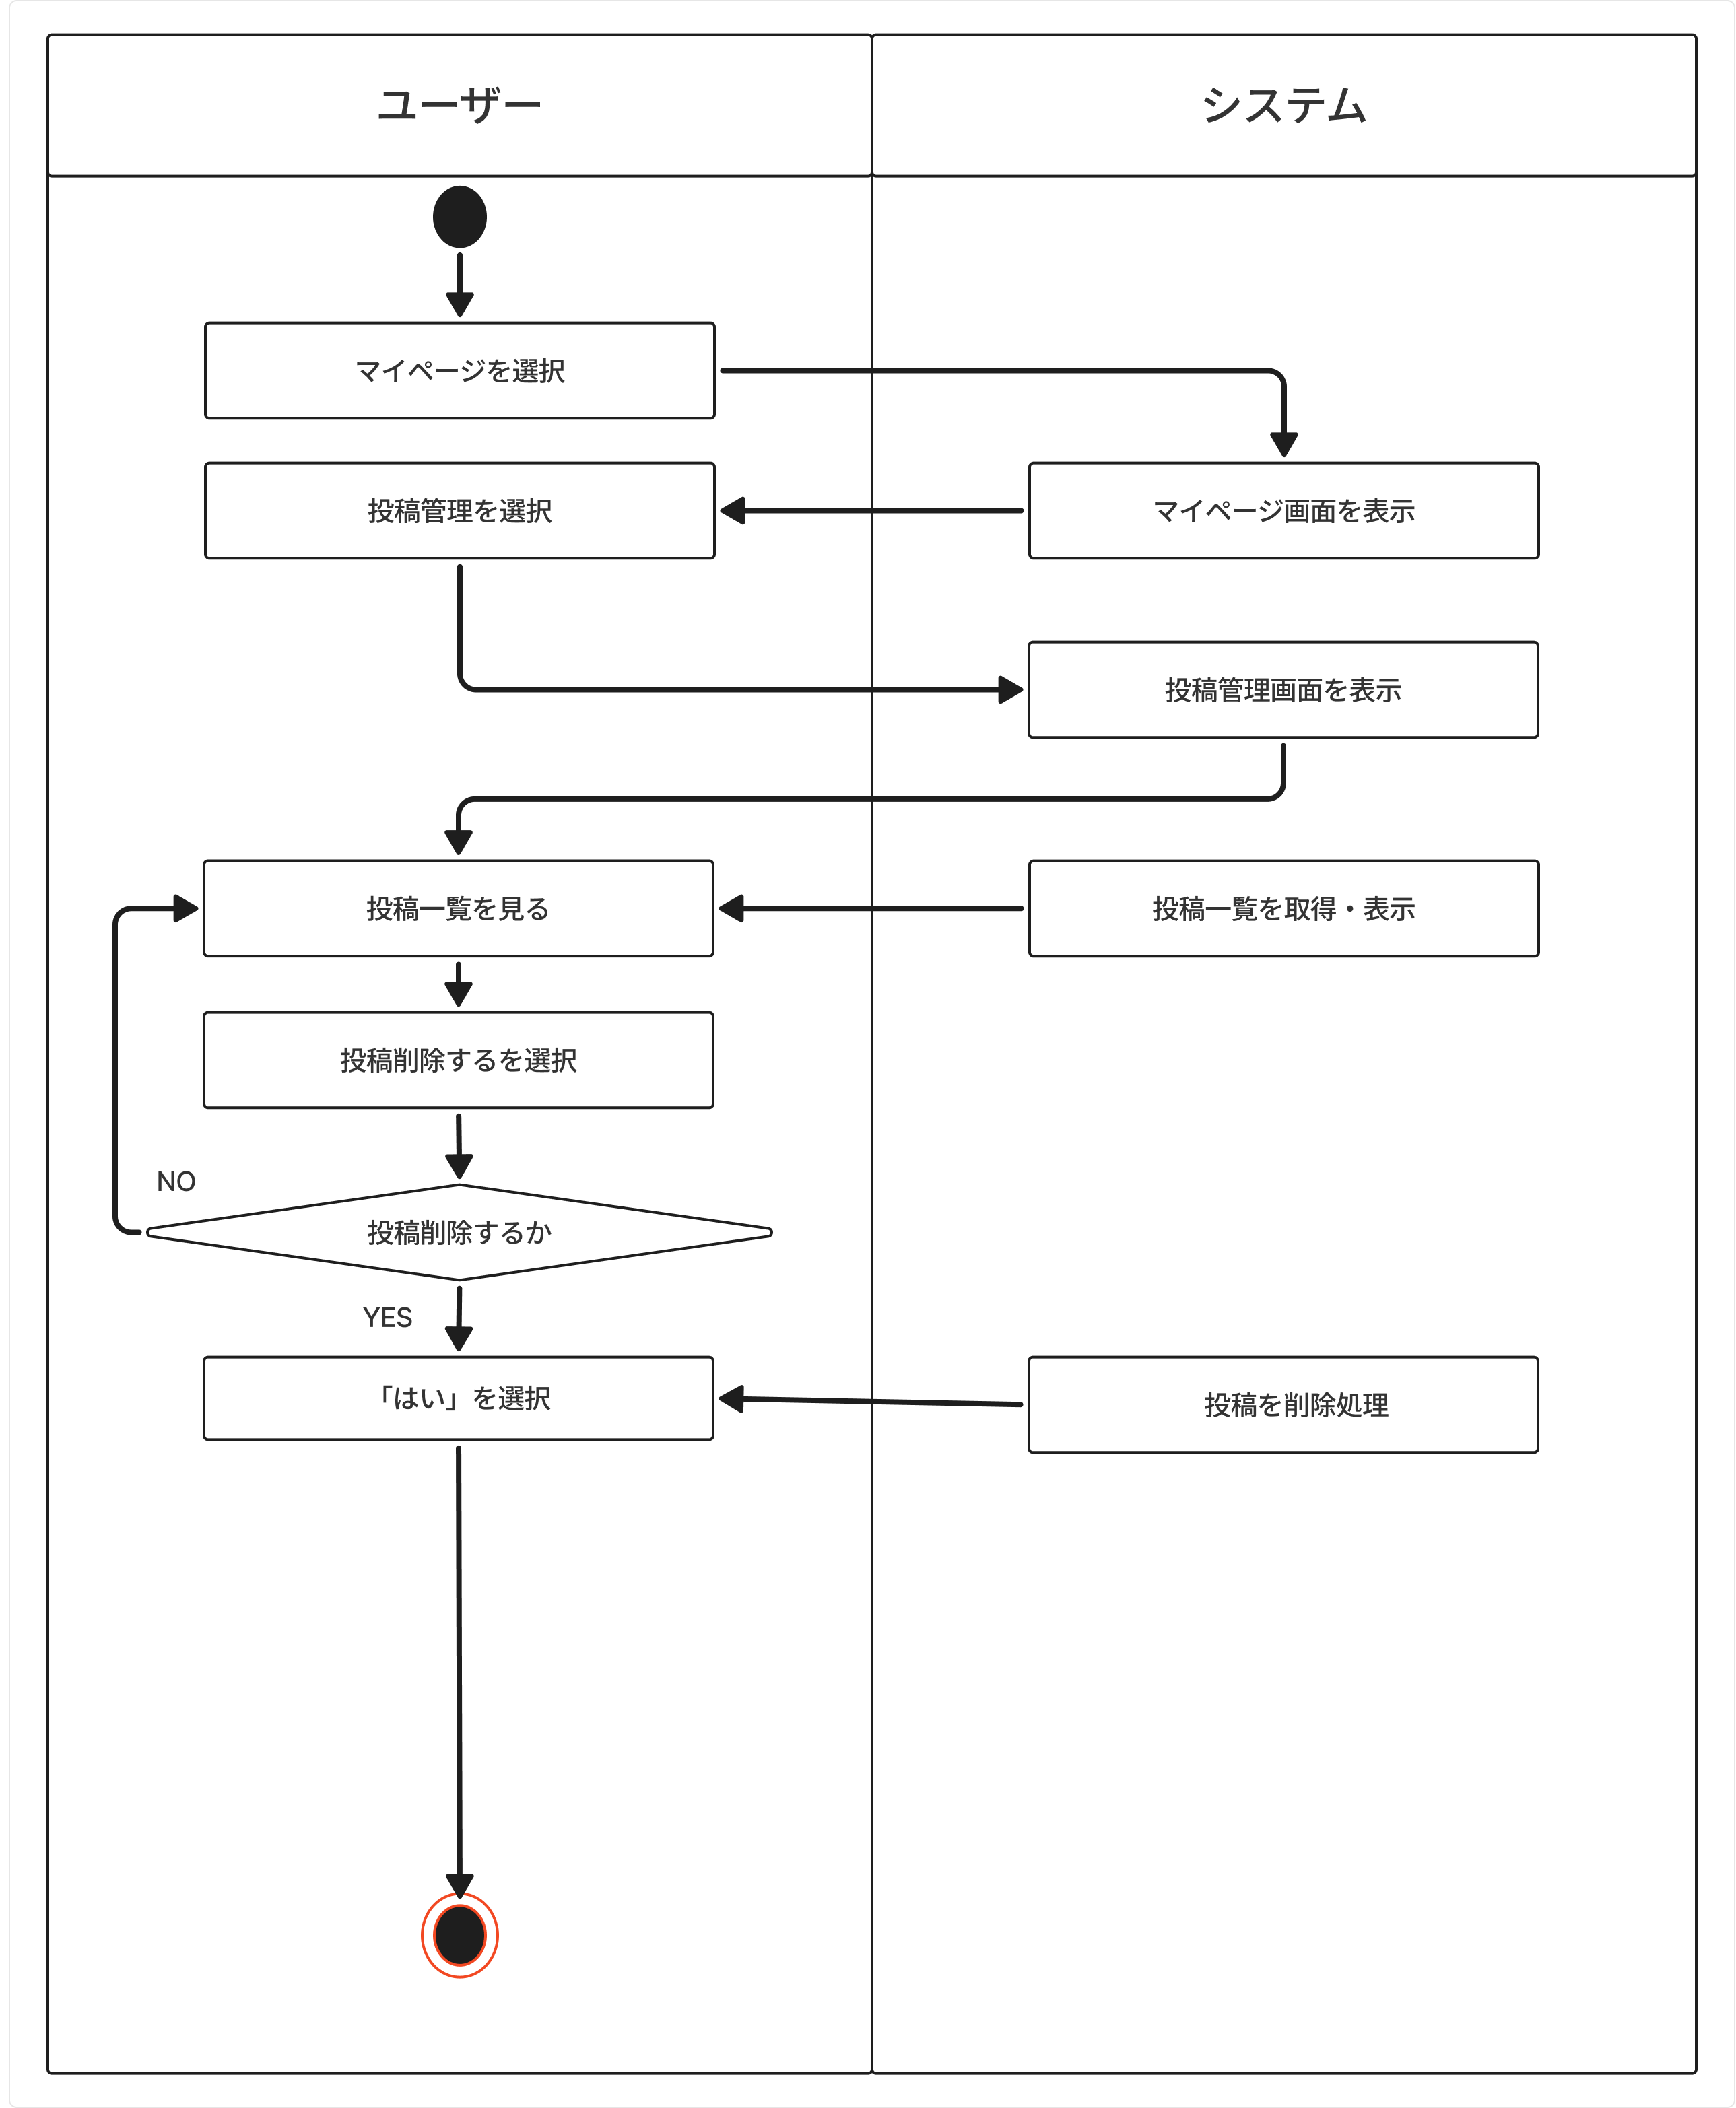
\includegraphics[width=0.5\textwidth]{chapters/images/e.png}
    \caption{投稿削除機能}
\end{figure}
\subsubsection{投稿編集機能}
本機能は、投稿の一覧から投稿を編集できる。
\begin{figure}[H]
    \centering
    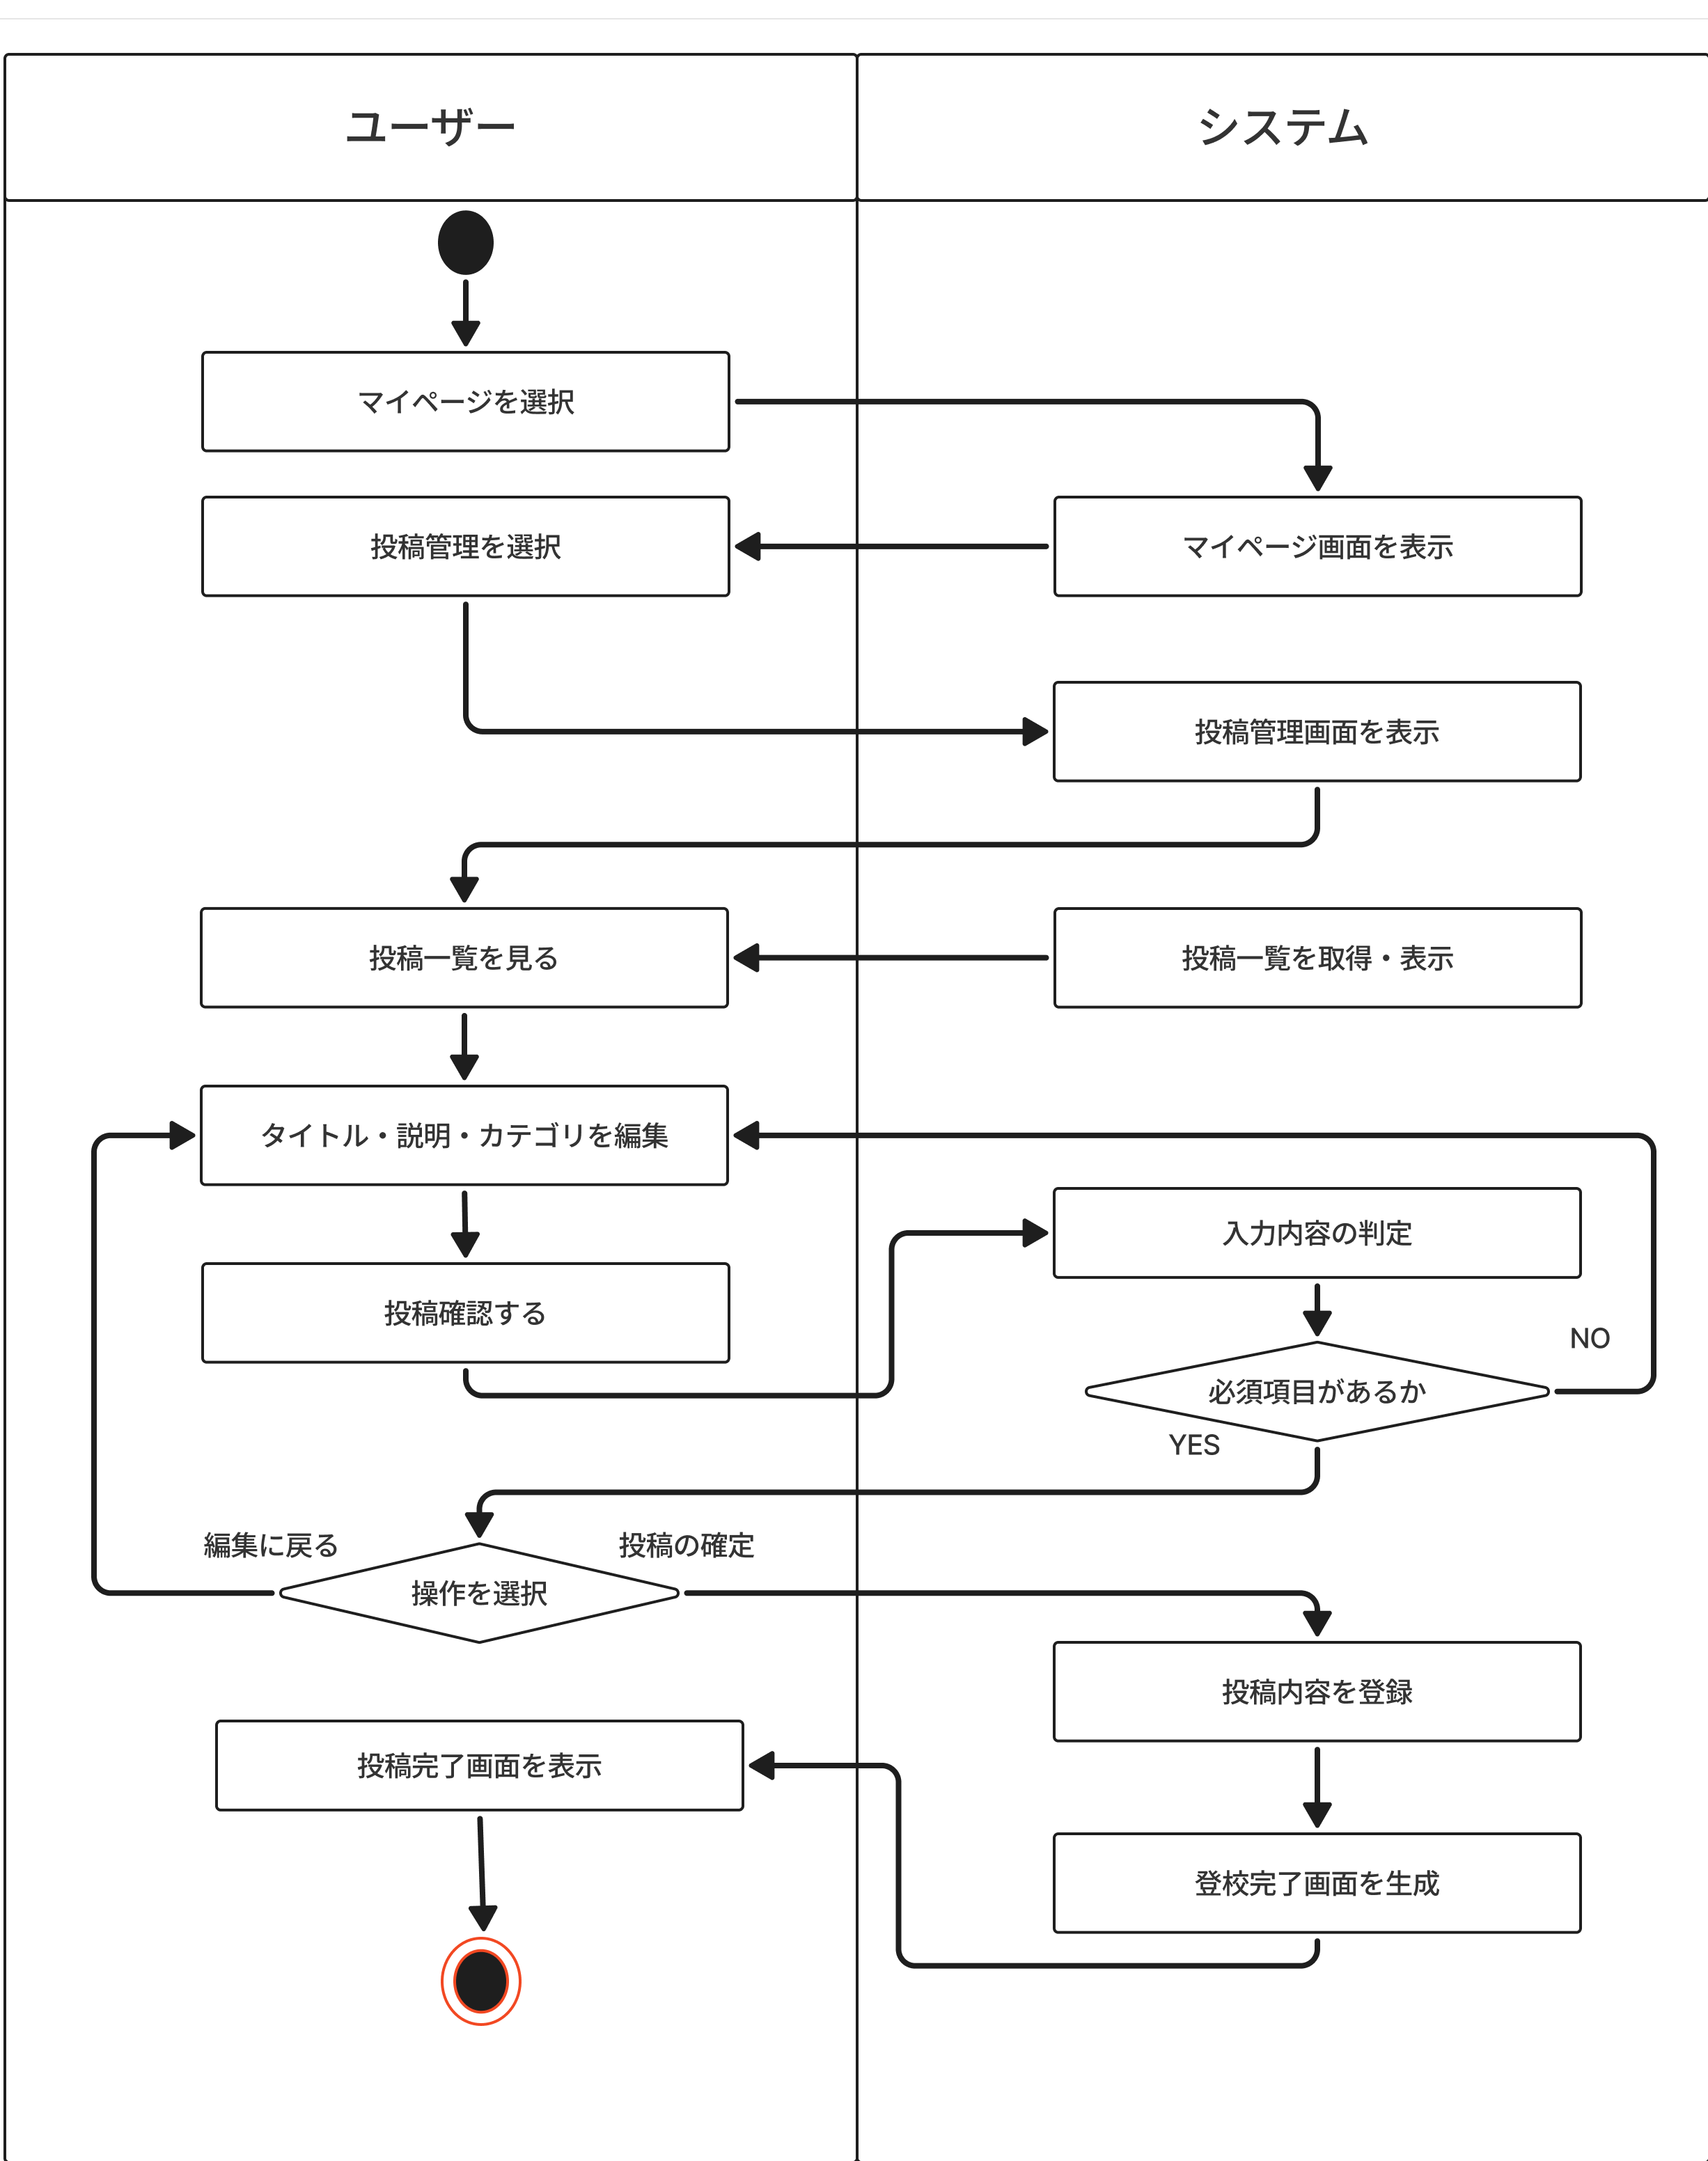
\includegraphics[width=0.5\textwidth]{chapters/images/f.png}
    \caption{投稿編集機能}
\end{figure}
\subsubsection{返信機能}
本機能は、投稿者の投稿メッセージに対して学習者が質問を通し理解を深める機能である。届いた質問が「回答済み」と「未回答」に分かれ一覧になっている。未回答の一覧のメッセージを選択すると回答可能となる。回答を終了した時「未回答」から「回答済み」にメッセージが移動する仕組みである。
\begin{figure}[H]
    \centering
    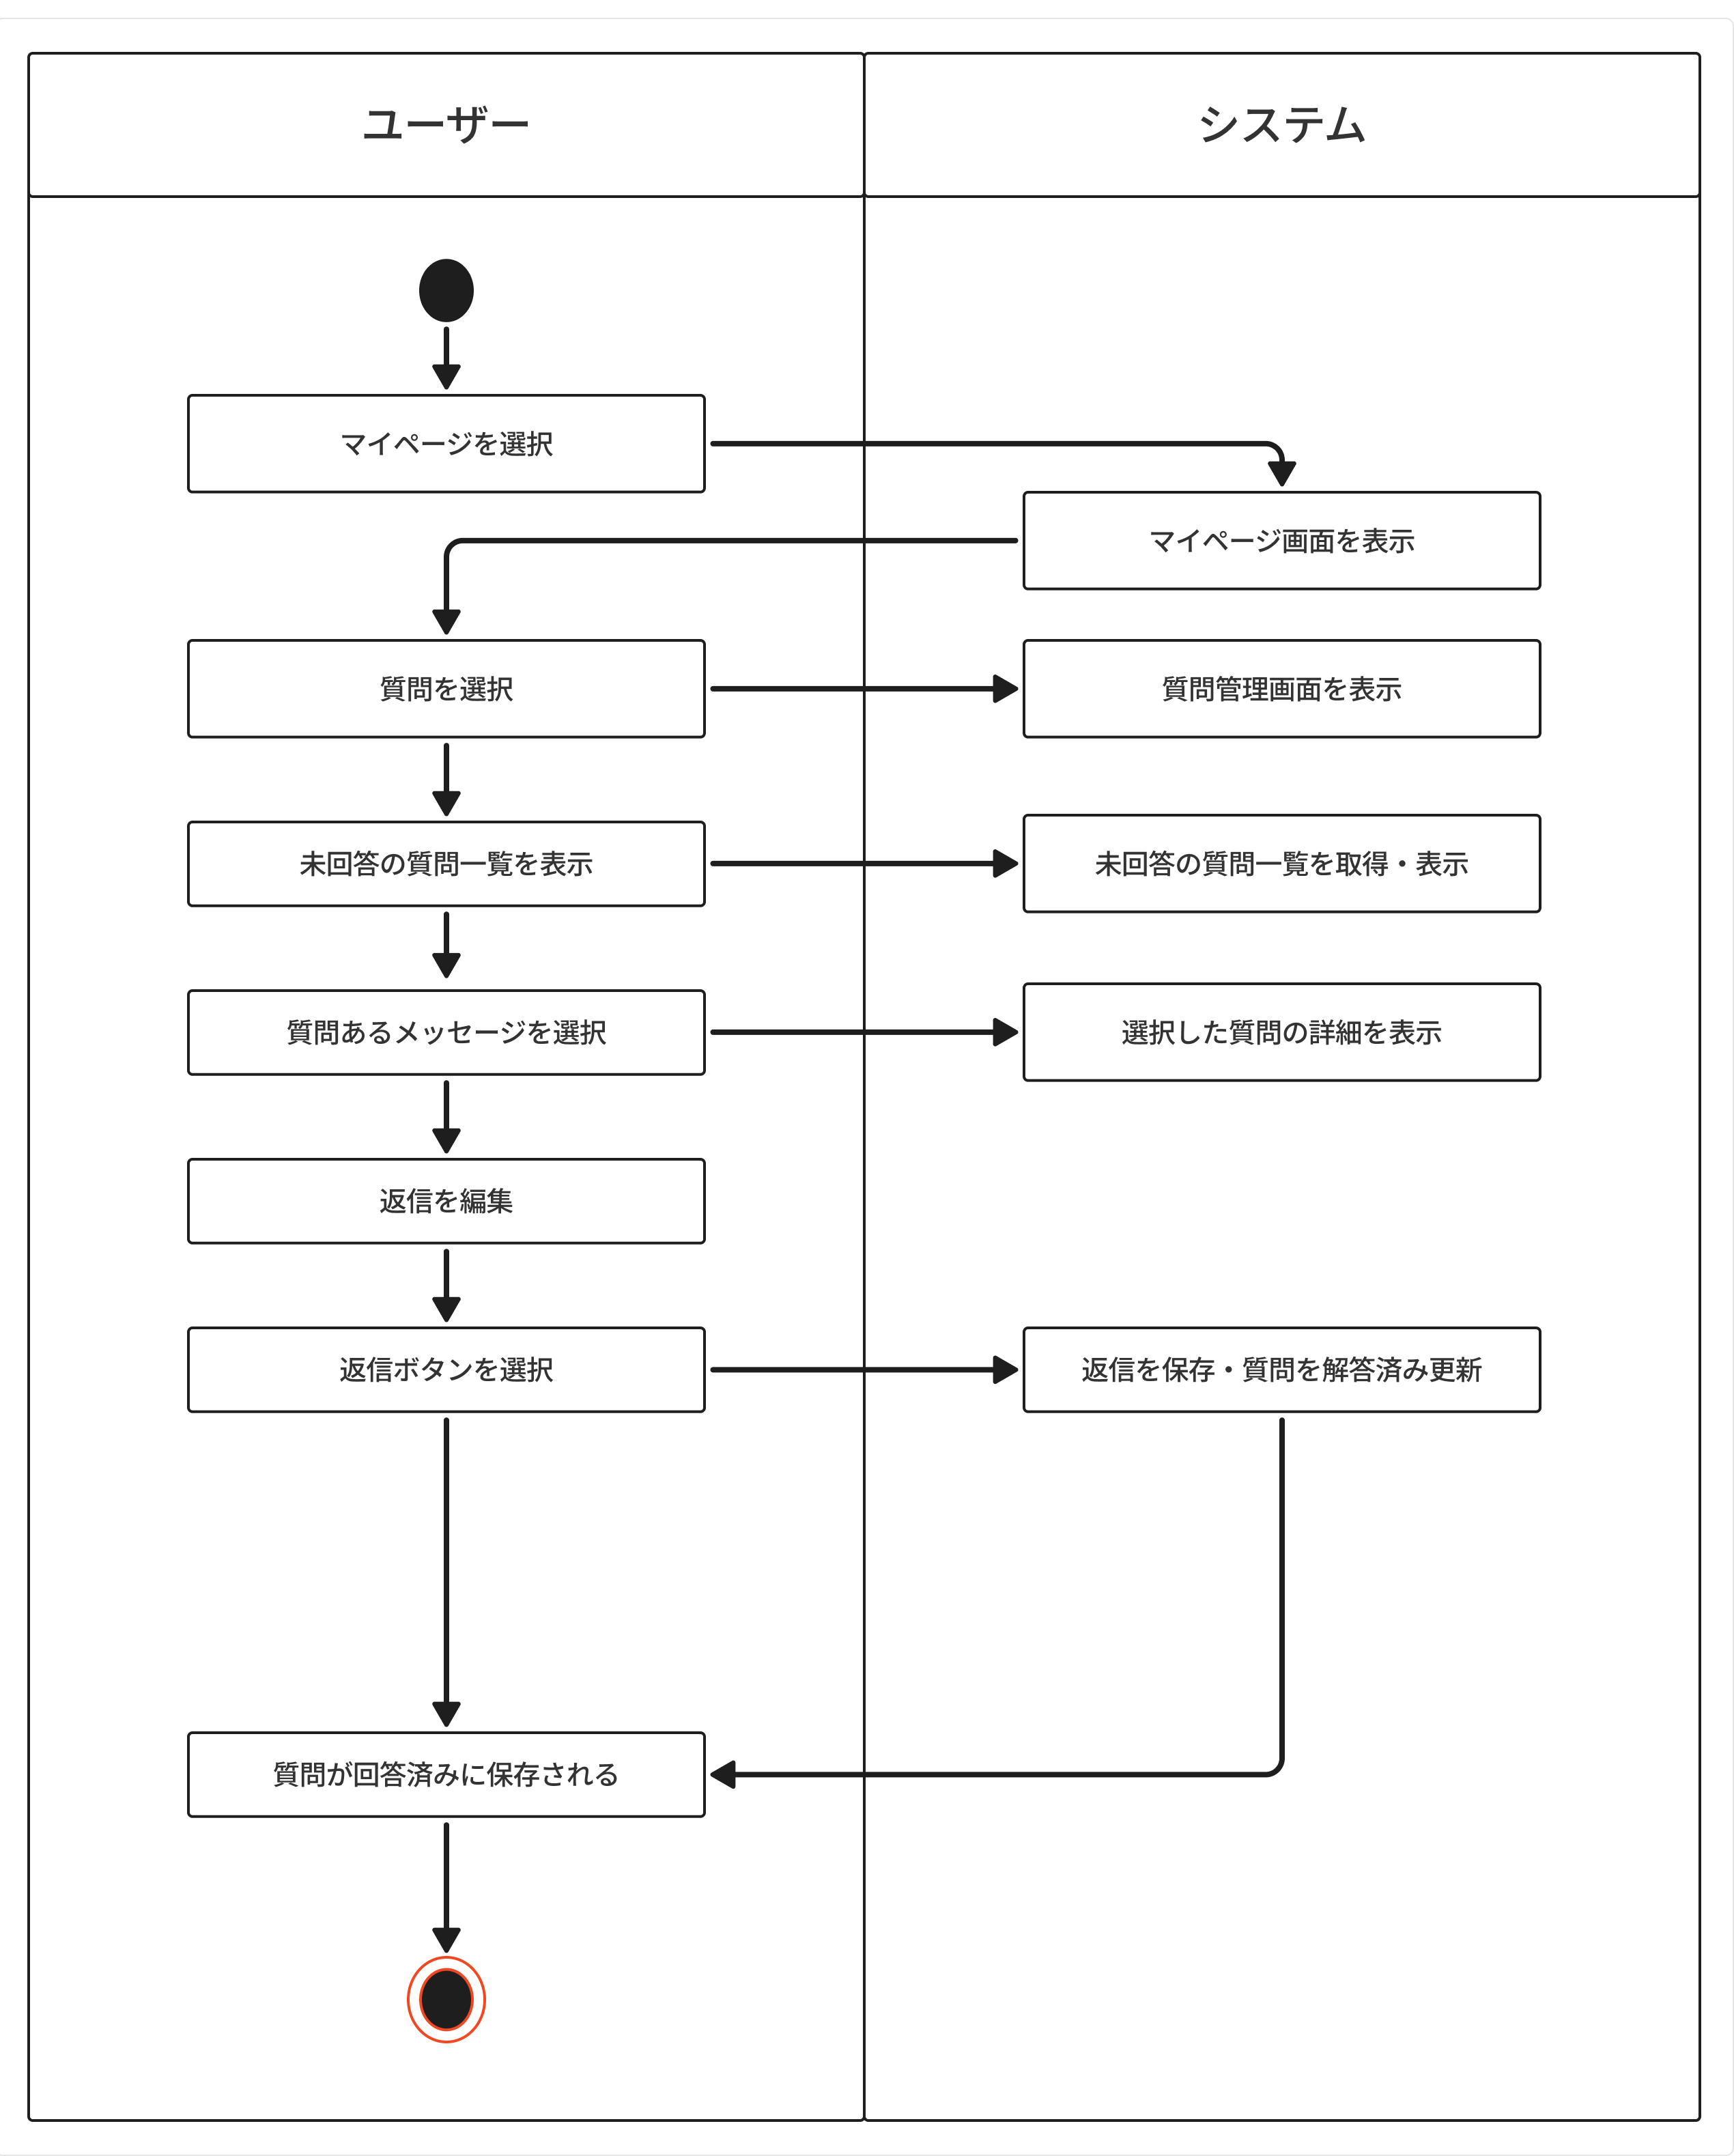
\includegraphics[width=0.5\textwidth]{chapters/images/g.png}
    \caption{返信機能}
\end{figure}
\subsubsection{プロフィール編集機能}
本機能は、プロフィール編集する機能である。
\begin{figure}[H]
    \centering
    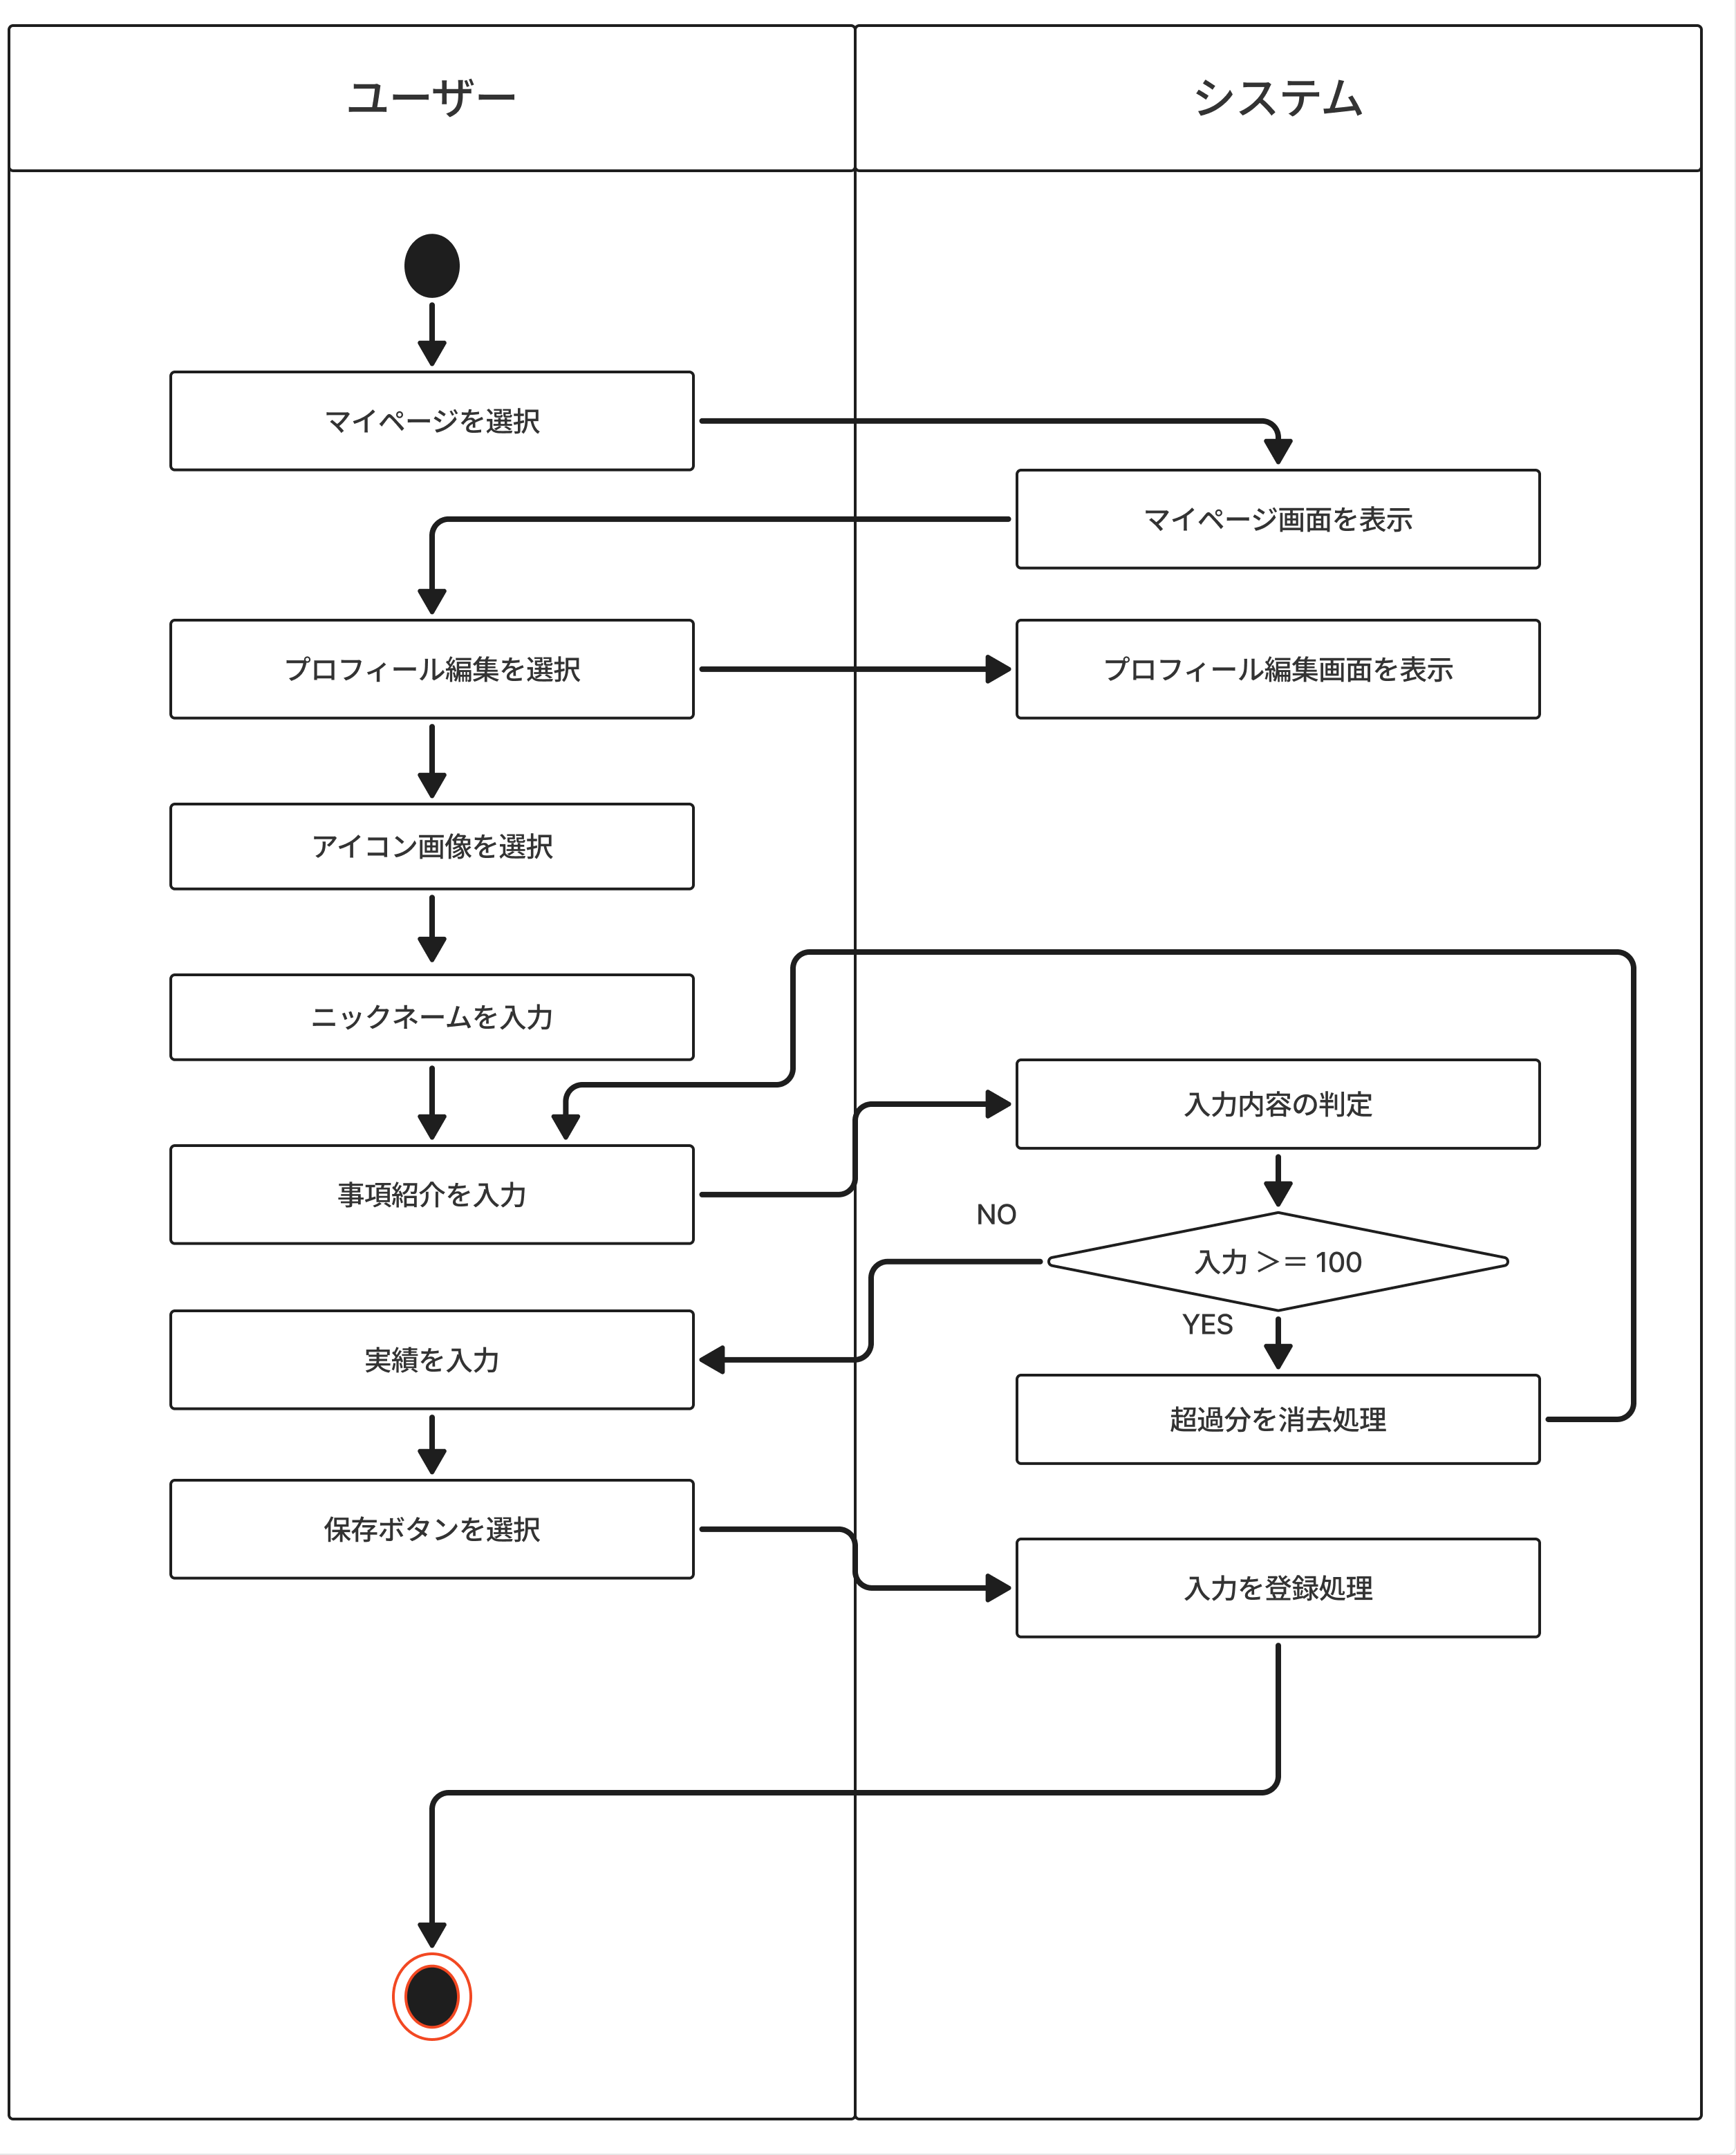
\includegraphics[width=0.5\textwidth]{chapters/images/h.png}
    \caption{プロフィール編集機能}
\end{figure}
\subsubsection{ログアウト機能}
本機能は、ログアウトする機能である。アカウントのログインした状態から解除されゲストモードに移行される。
\begin{figure}[H]
    \centering
    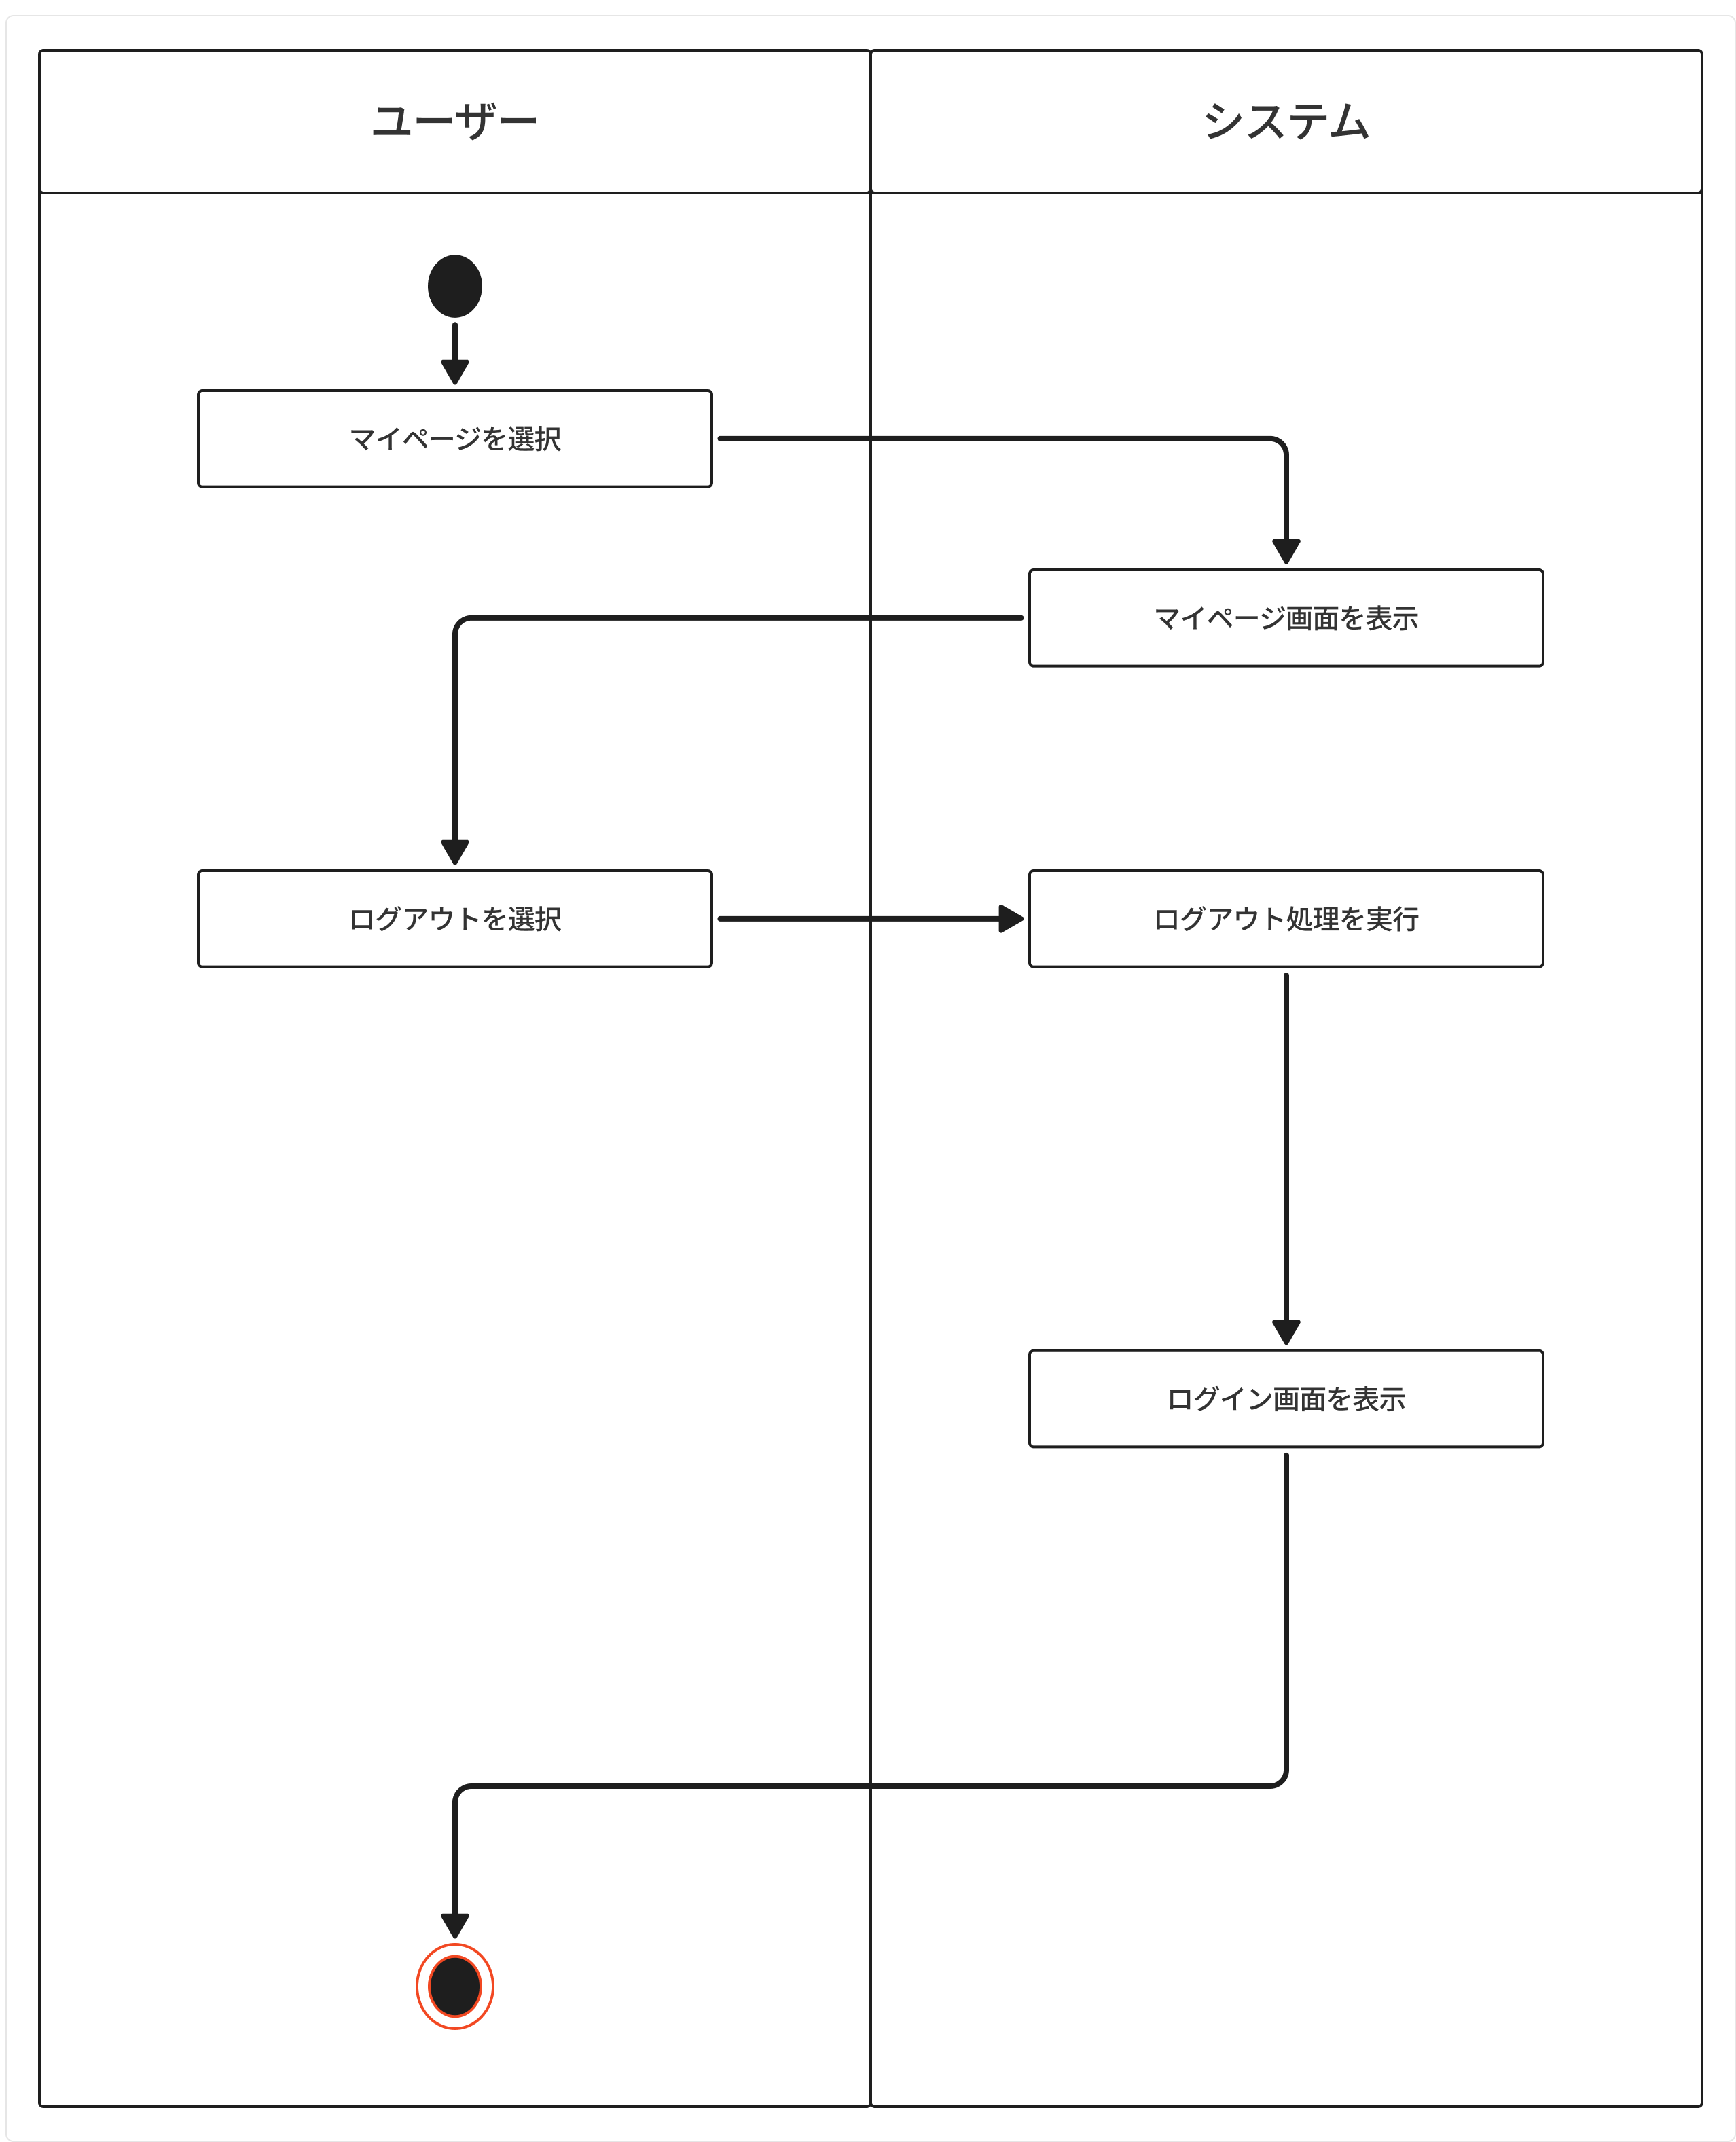
\includegraphics[width=0.5\textwidth]{chapters/images/i.png}
    \caption{ログアウト機能}
\end{figure}
\subsubsection{ありがとうの木機能}
本機能は、投稿者を視覚的に評価するための「ありがとうの木」機能です。学習者がメッセージに♡を押したとき投稿者のマイページ画面のありがとうの木が成長していく。
\begin{figure}[H]
    \centering
    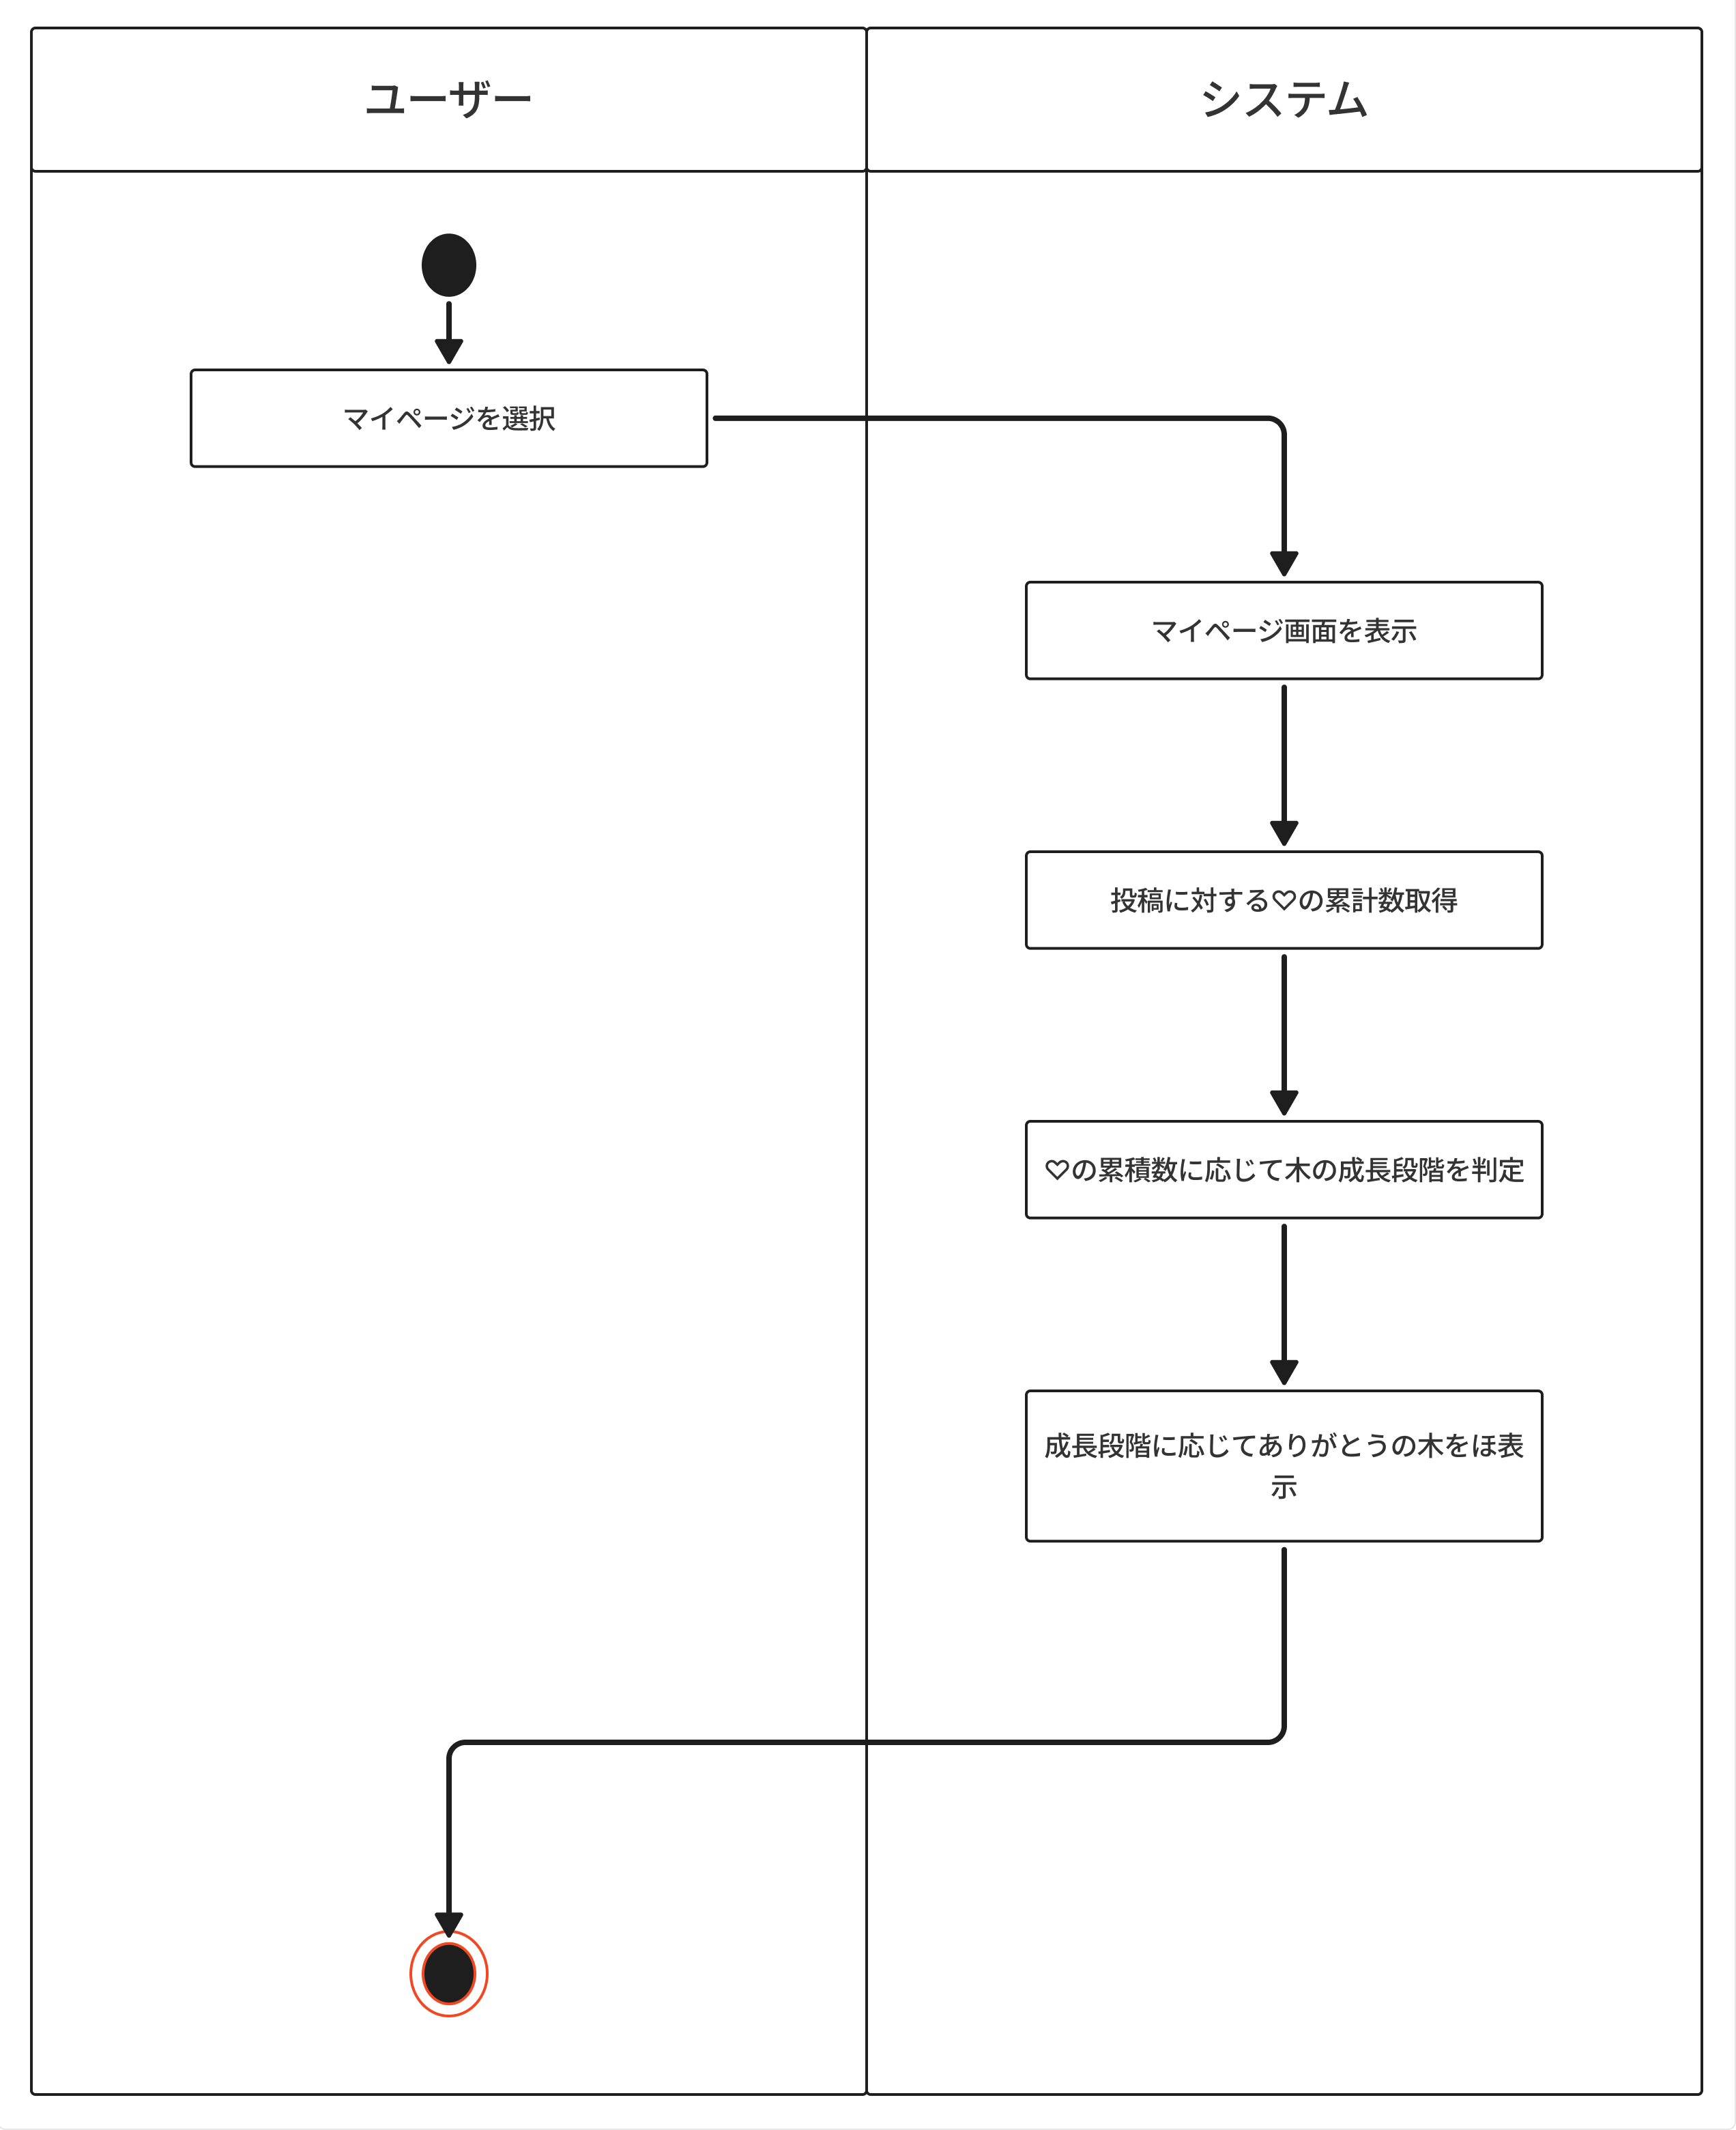
\includegraphics[width=0.5\textwidth]{chapters/images/j.png}
    \caption{ありがとうの木機能}
\end{figure}
\subsubsection{ランク機能}
本機能は、投稿者を視覚的に評価するための「ありがとうの木」機能です。学習者がメッセージに♡を押したとき投稿者のマイページ画面のありがとうの木が成長していく。
\begin{figure}[H]
    \centering
    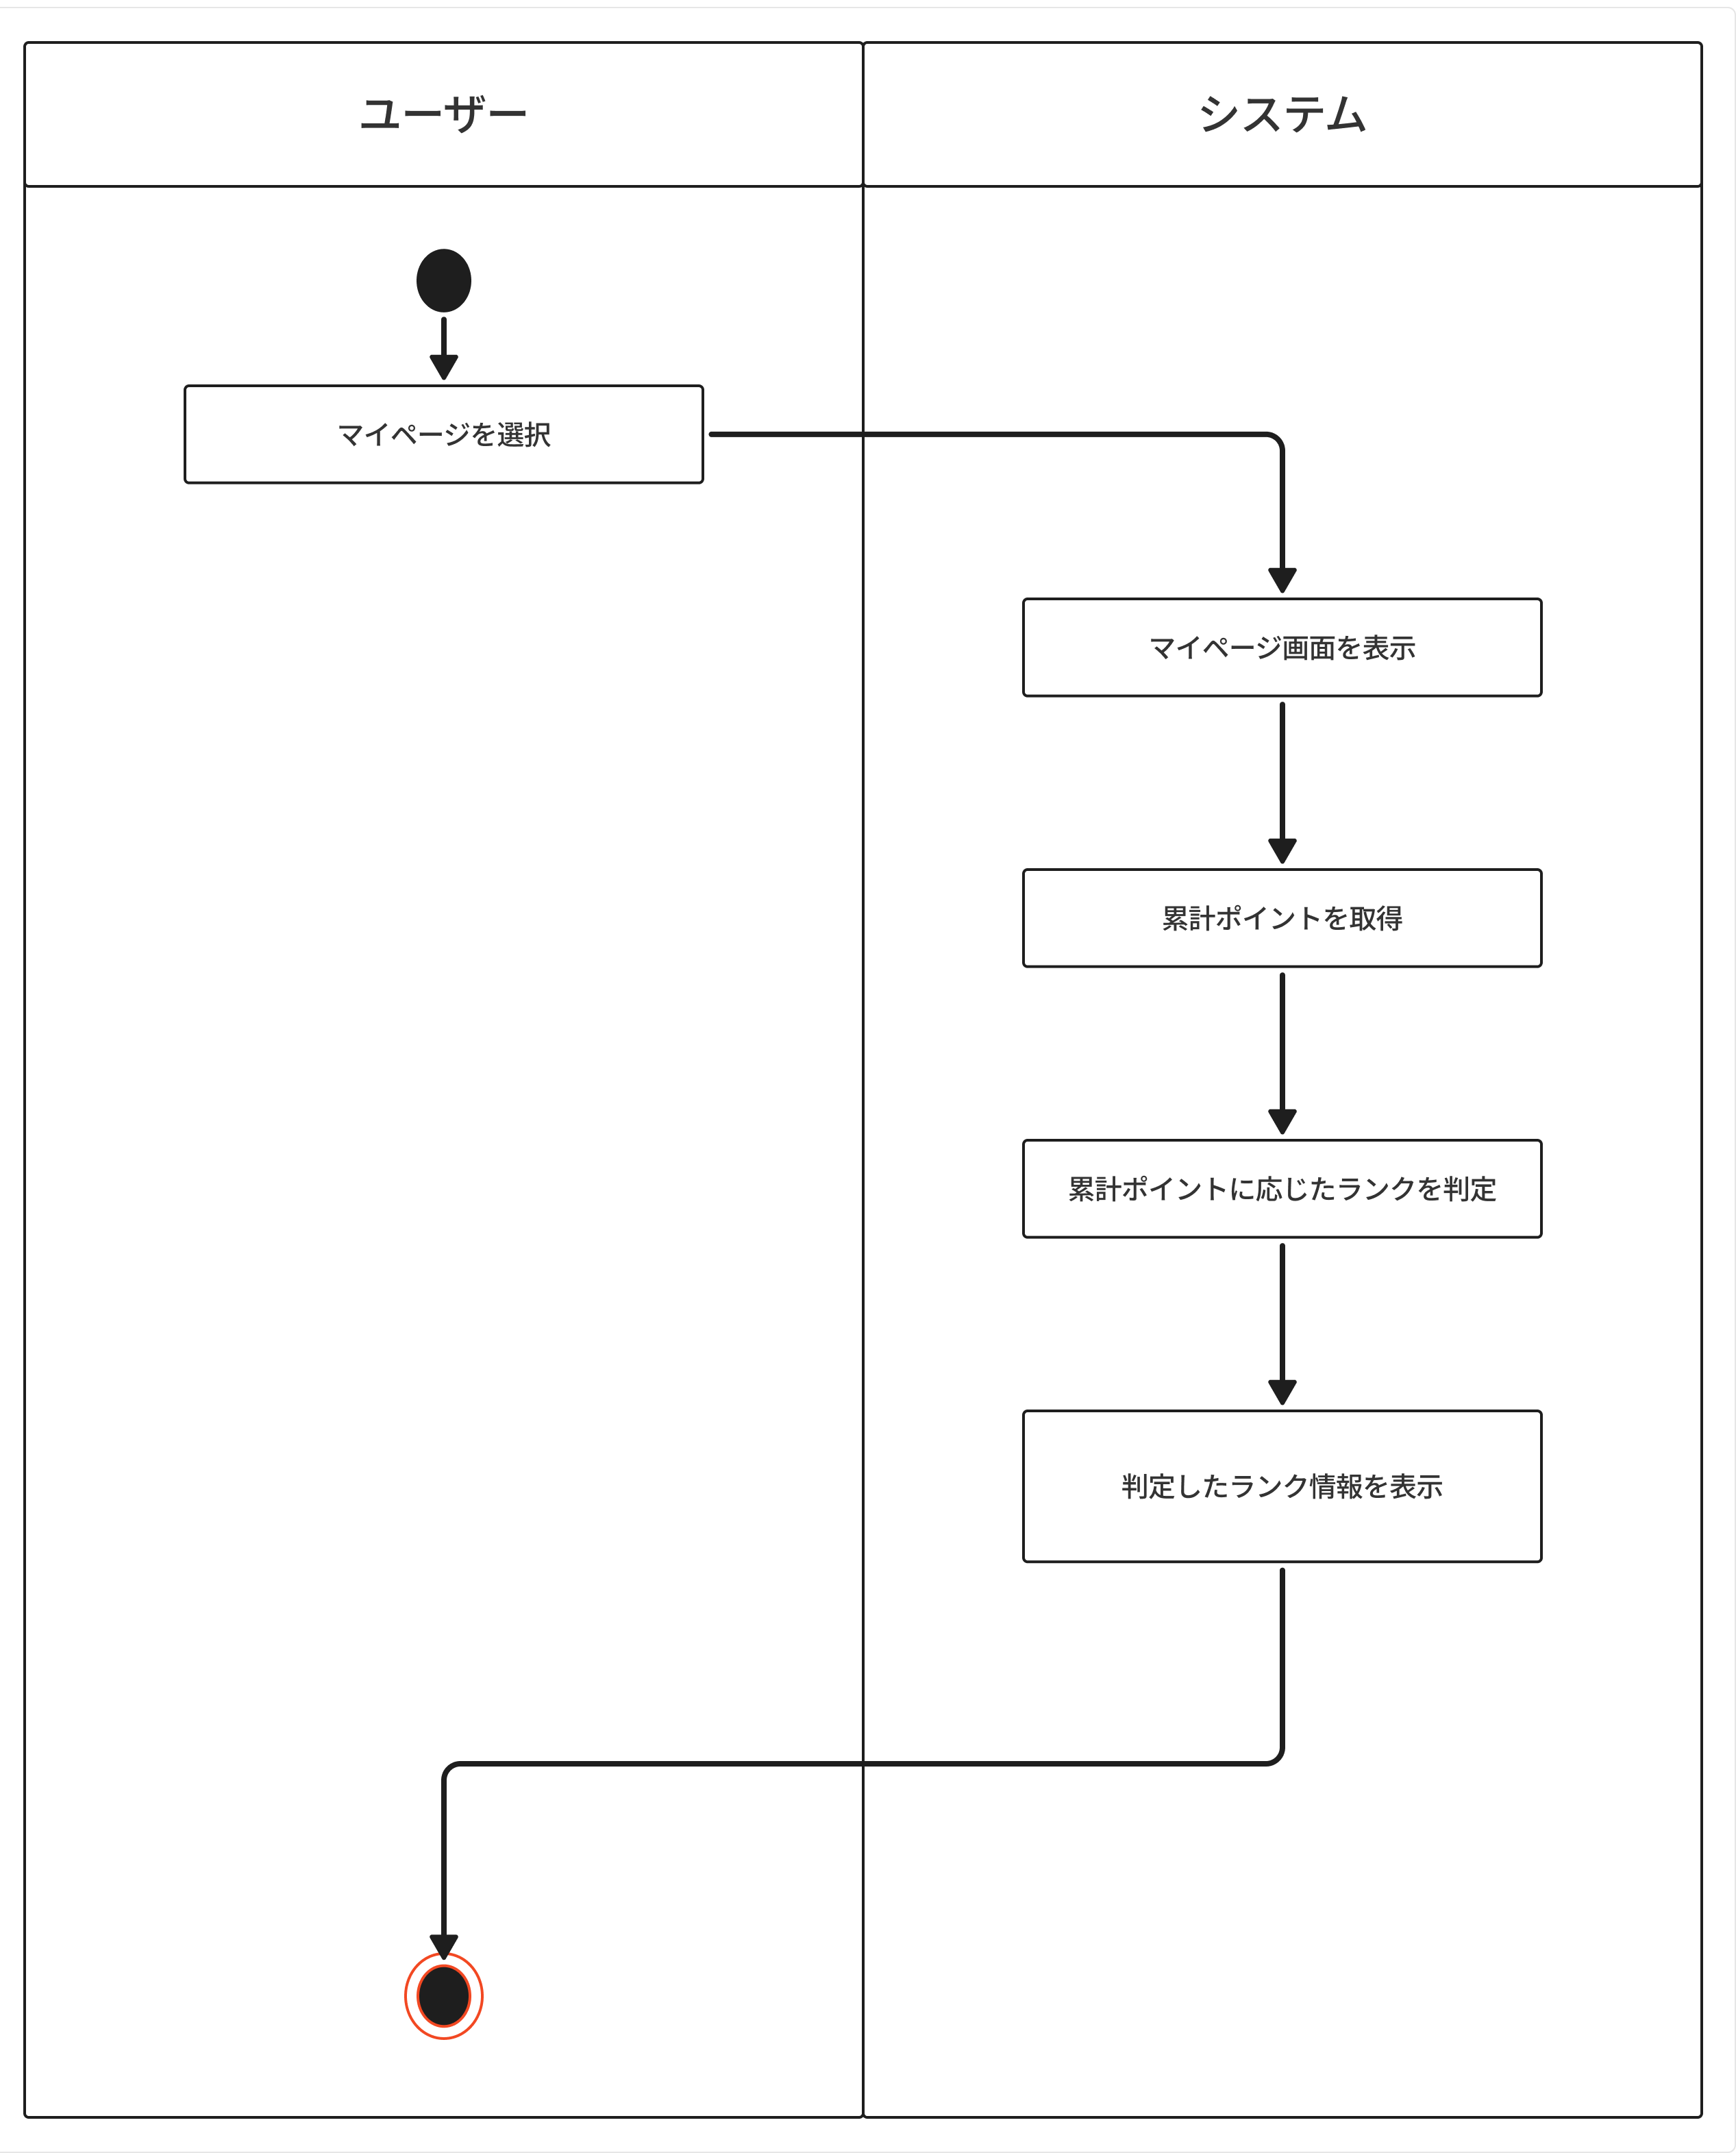
\includegraphics[width=0.5\textwidth]{chapters/images/k.png}
    \caption{ランク機能}
\end{figure}
\subsubsection{ランキング機能}
本機能は、投稿表を視覚的に評価するための「ランキング」機能である。ポイントの累計からランキングをつける。
\begin{figure}[H]
    \centering
    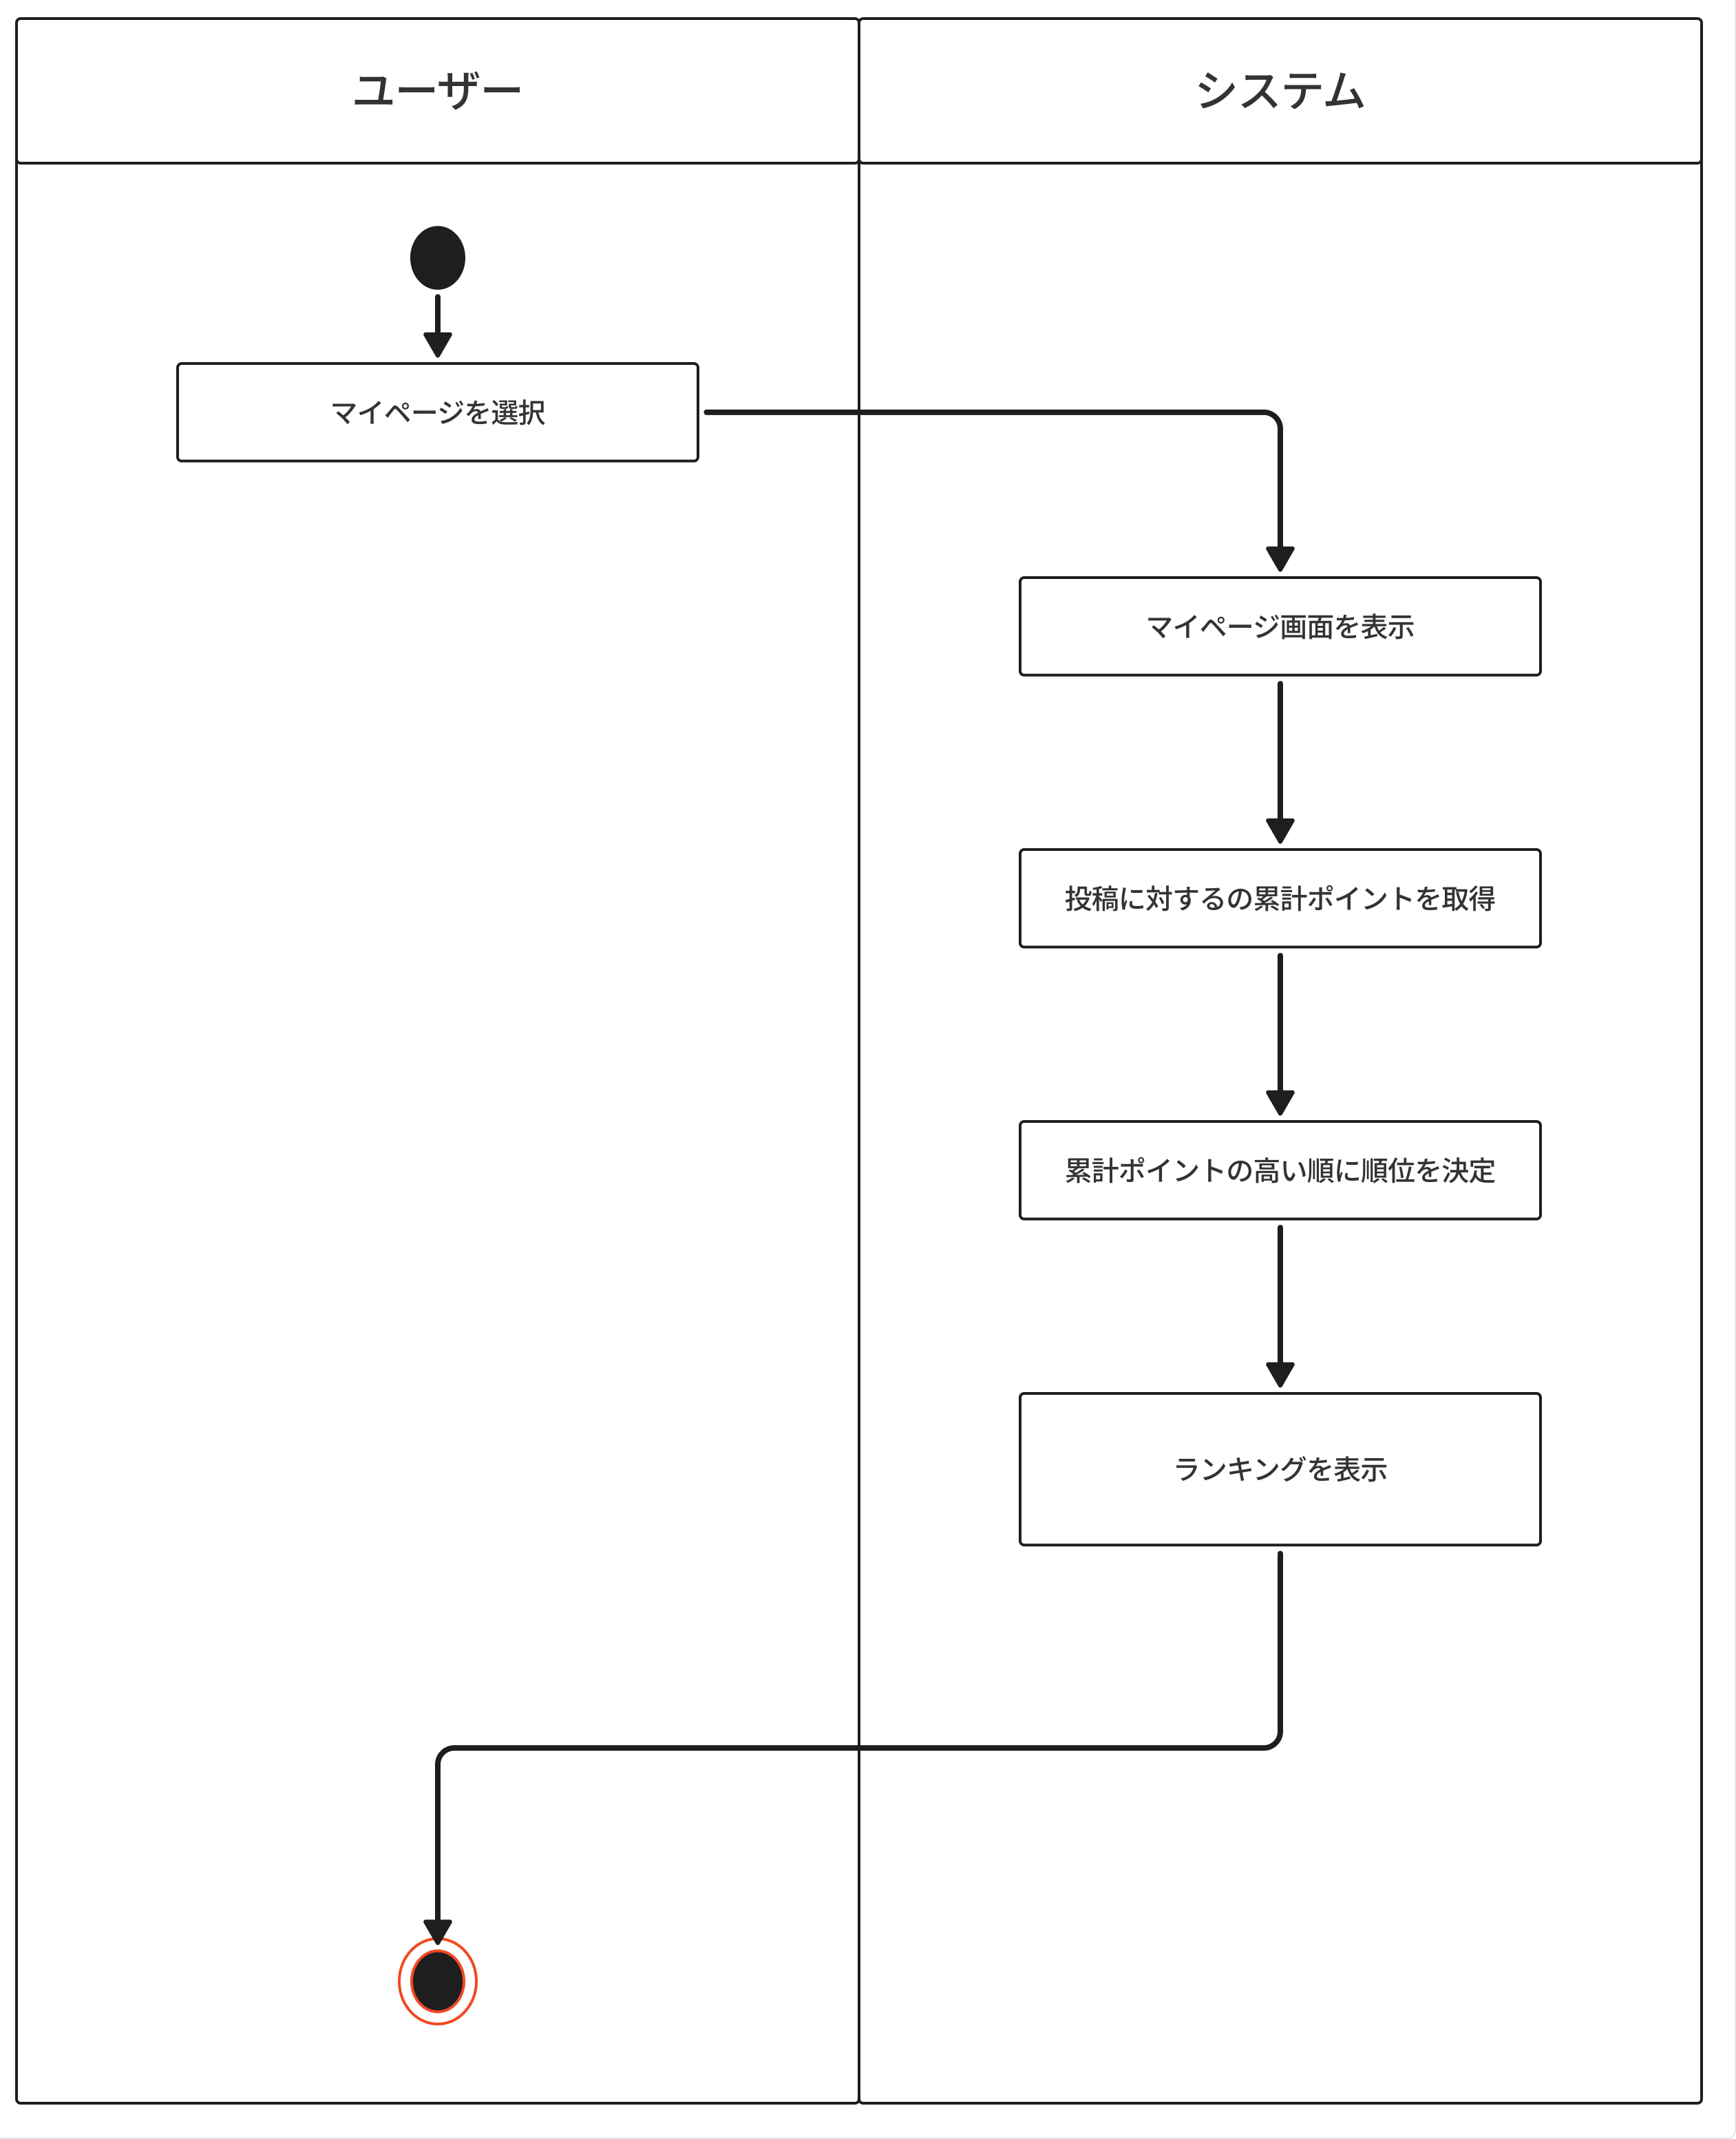
\includegraphics[width=0.5\textwidth]{chapters/images/l.png}
    \caption{ランキング機能}
\end{figure}
\subsubsection{一定ポイント付与機能}
本機能は、投稿者を視覚的に評価するための「ランキング」機能のためのポイント付与機能。このポイントの累計からランキングをつける。投稿した時一定のポイントが付与され、マイページにて確認できる。
\begin{figure}[H]
    \centering
    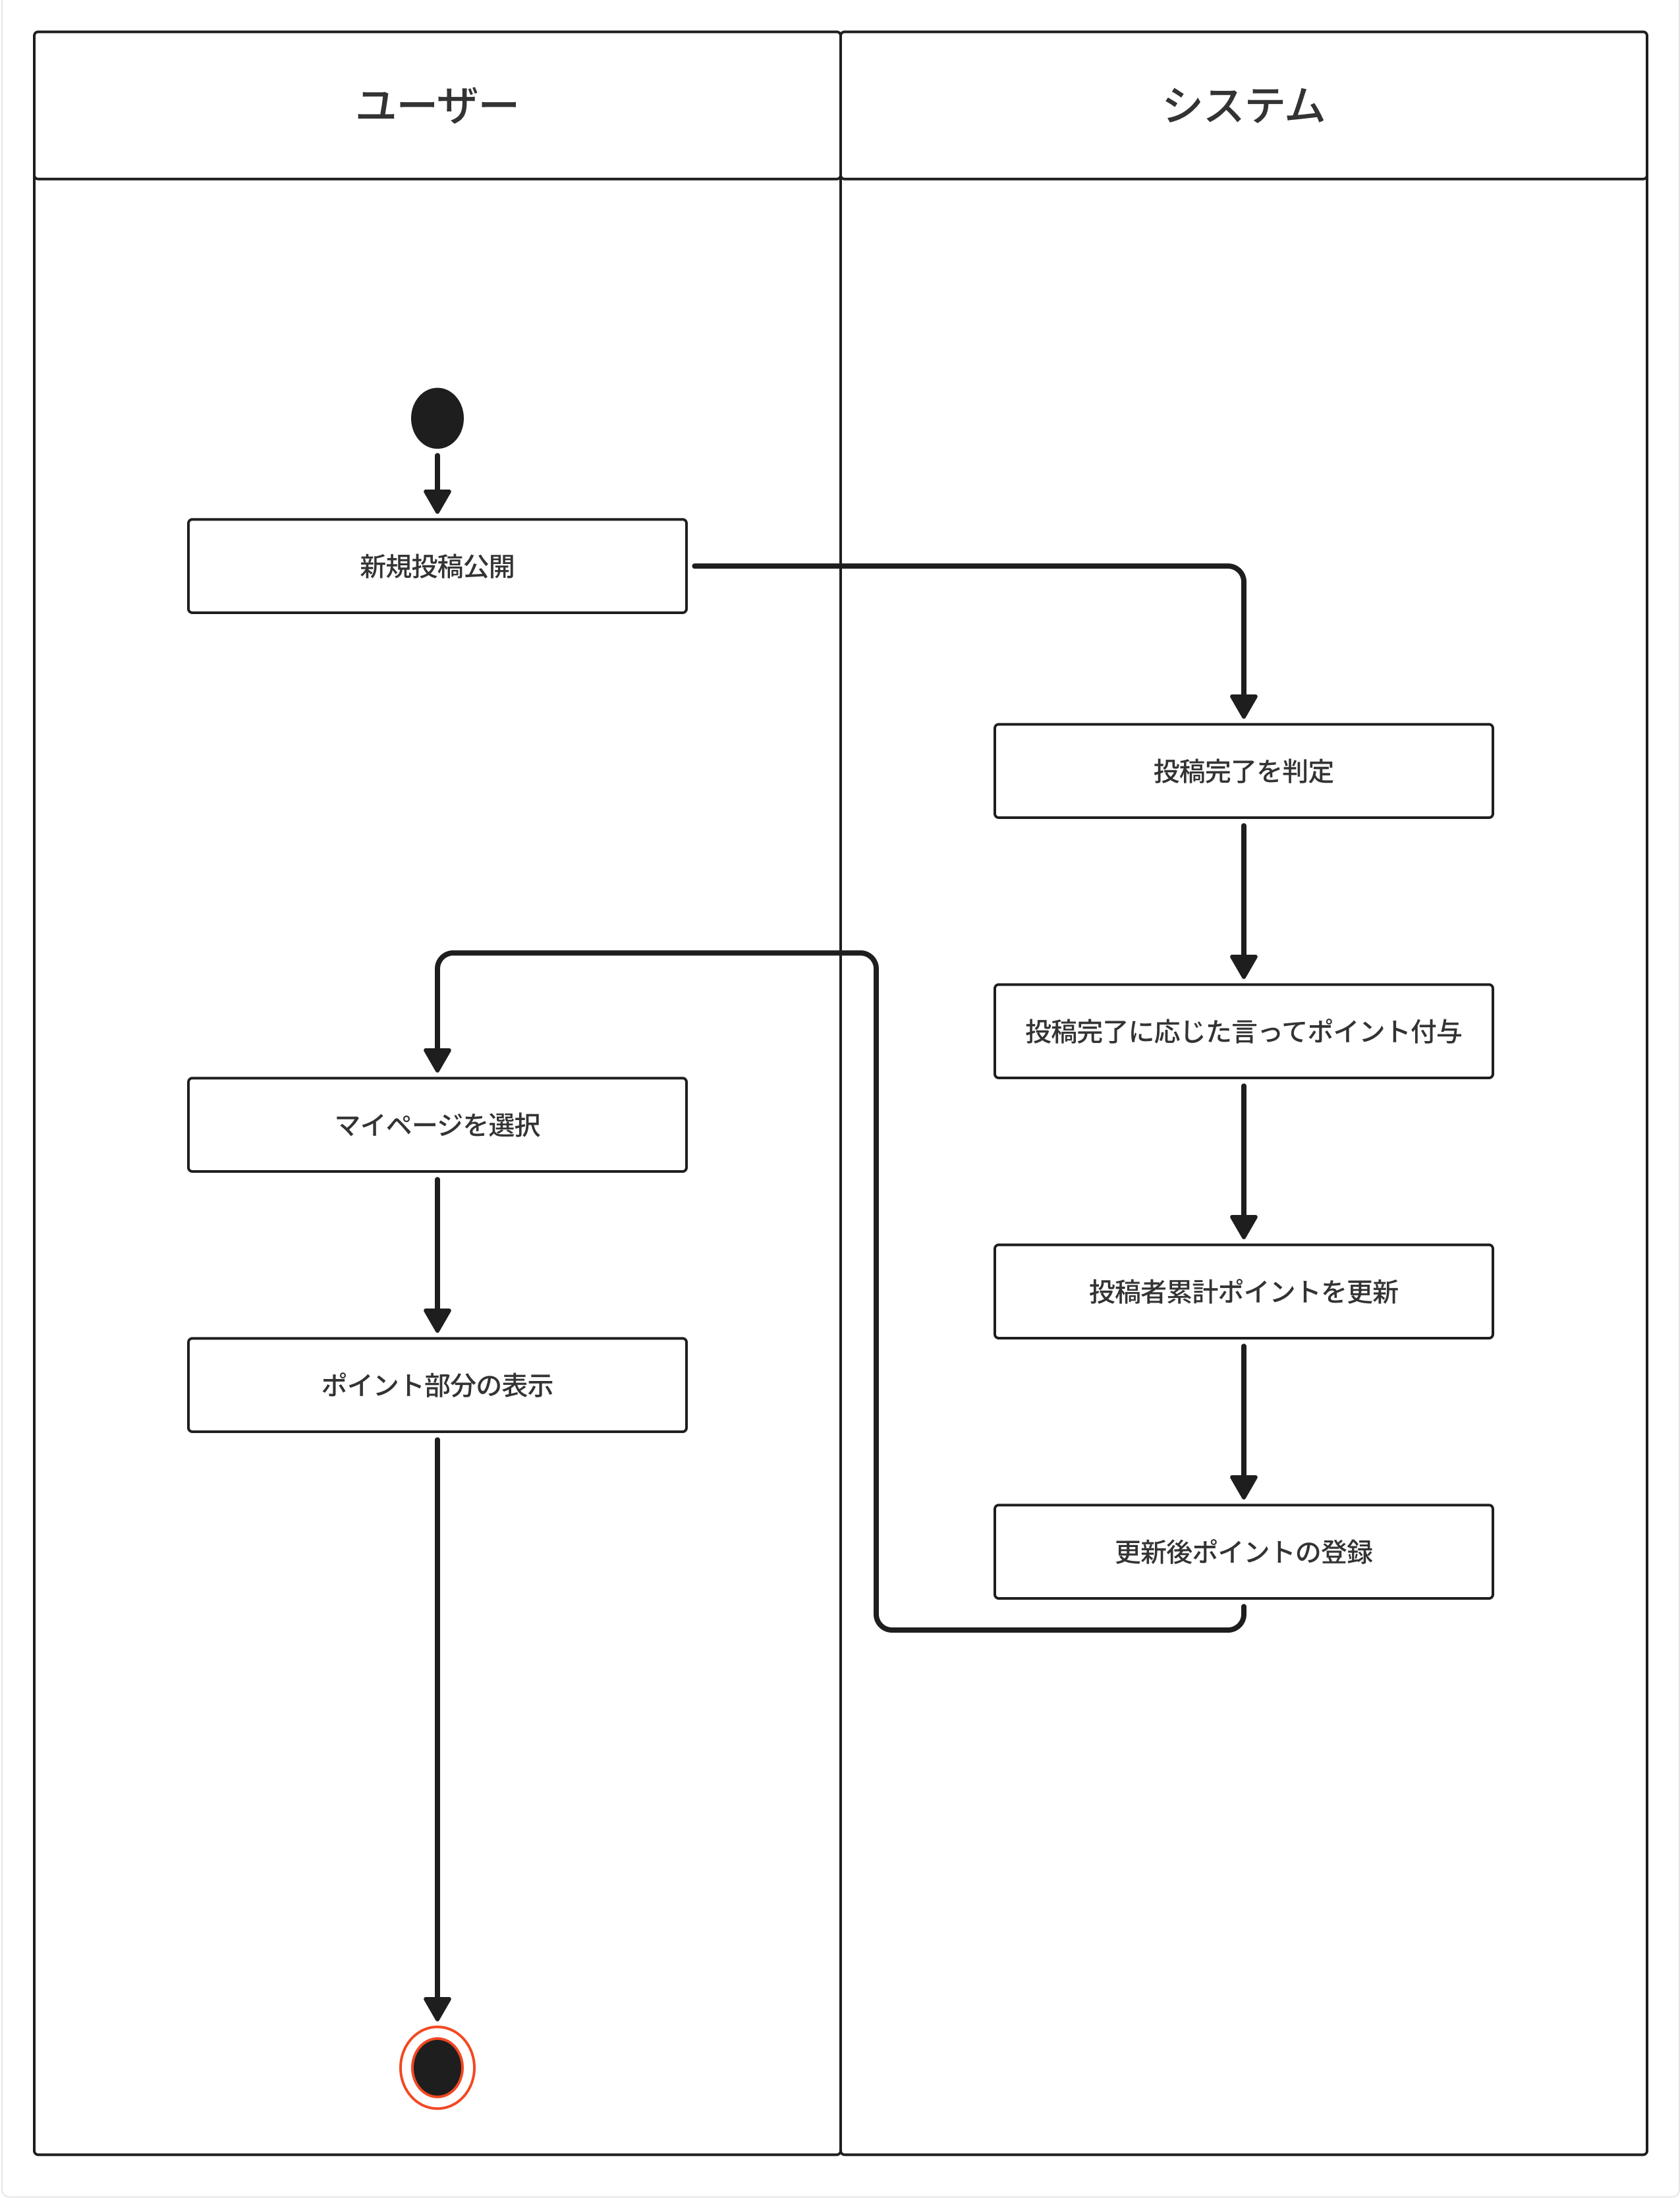
\includegraphics[width=0.5\textwidth]{chapters/images/m.png}
    \caption{一定ポイント付与機能}
\end{figure}
\subsubsection{♡によるポイント付与機能}
本機能は、投稿者を視覚的に評価するための「ランキング」機能のためのポイント付与機能。このポイントの累計からランキングをつける。♡が押されたとき追加ポイントが付与され、マイページにて確認できる。
\begin{figure}[H]
    \centering
    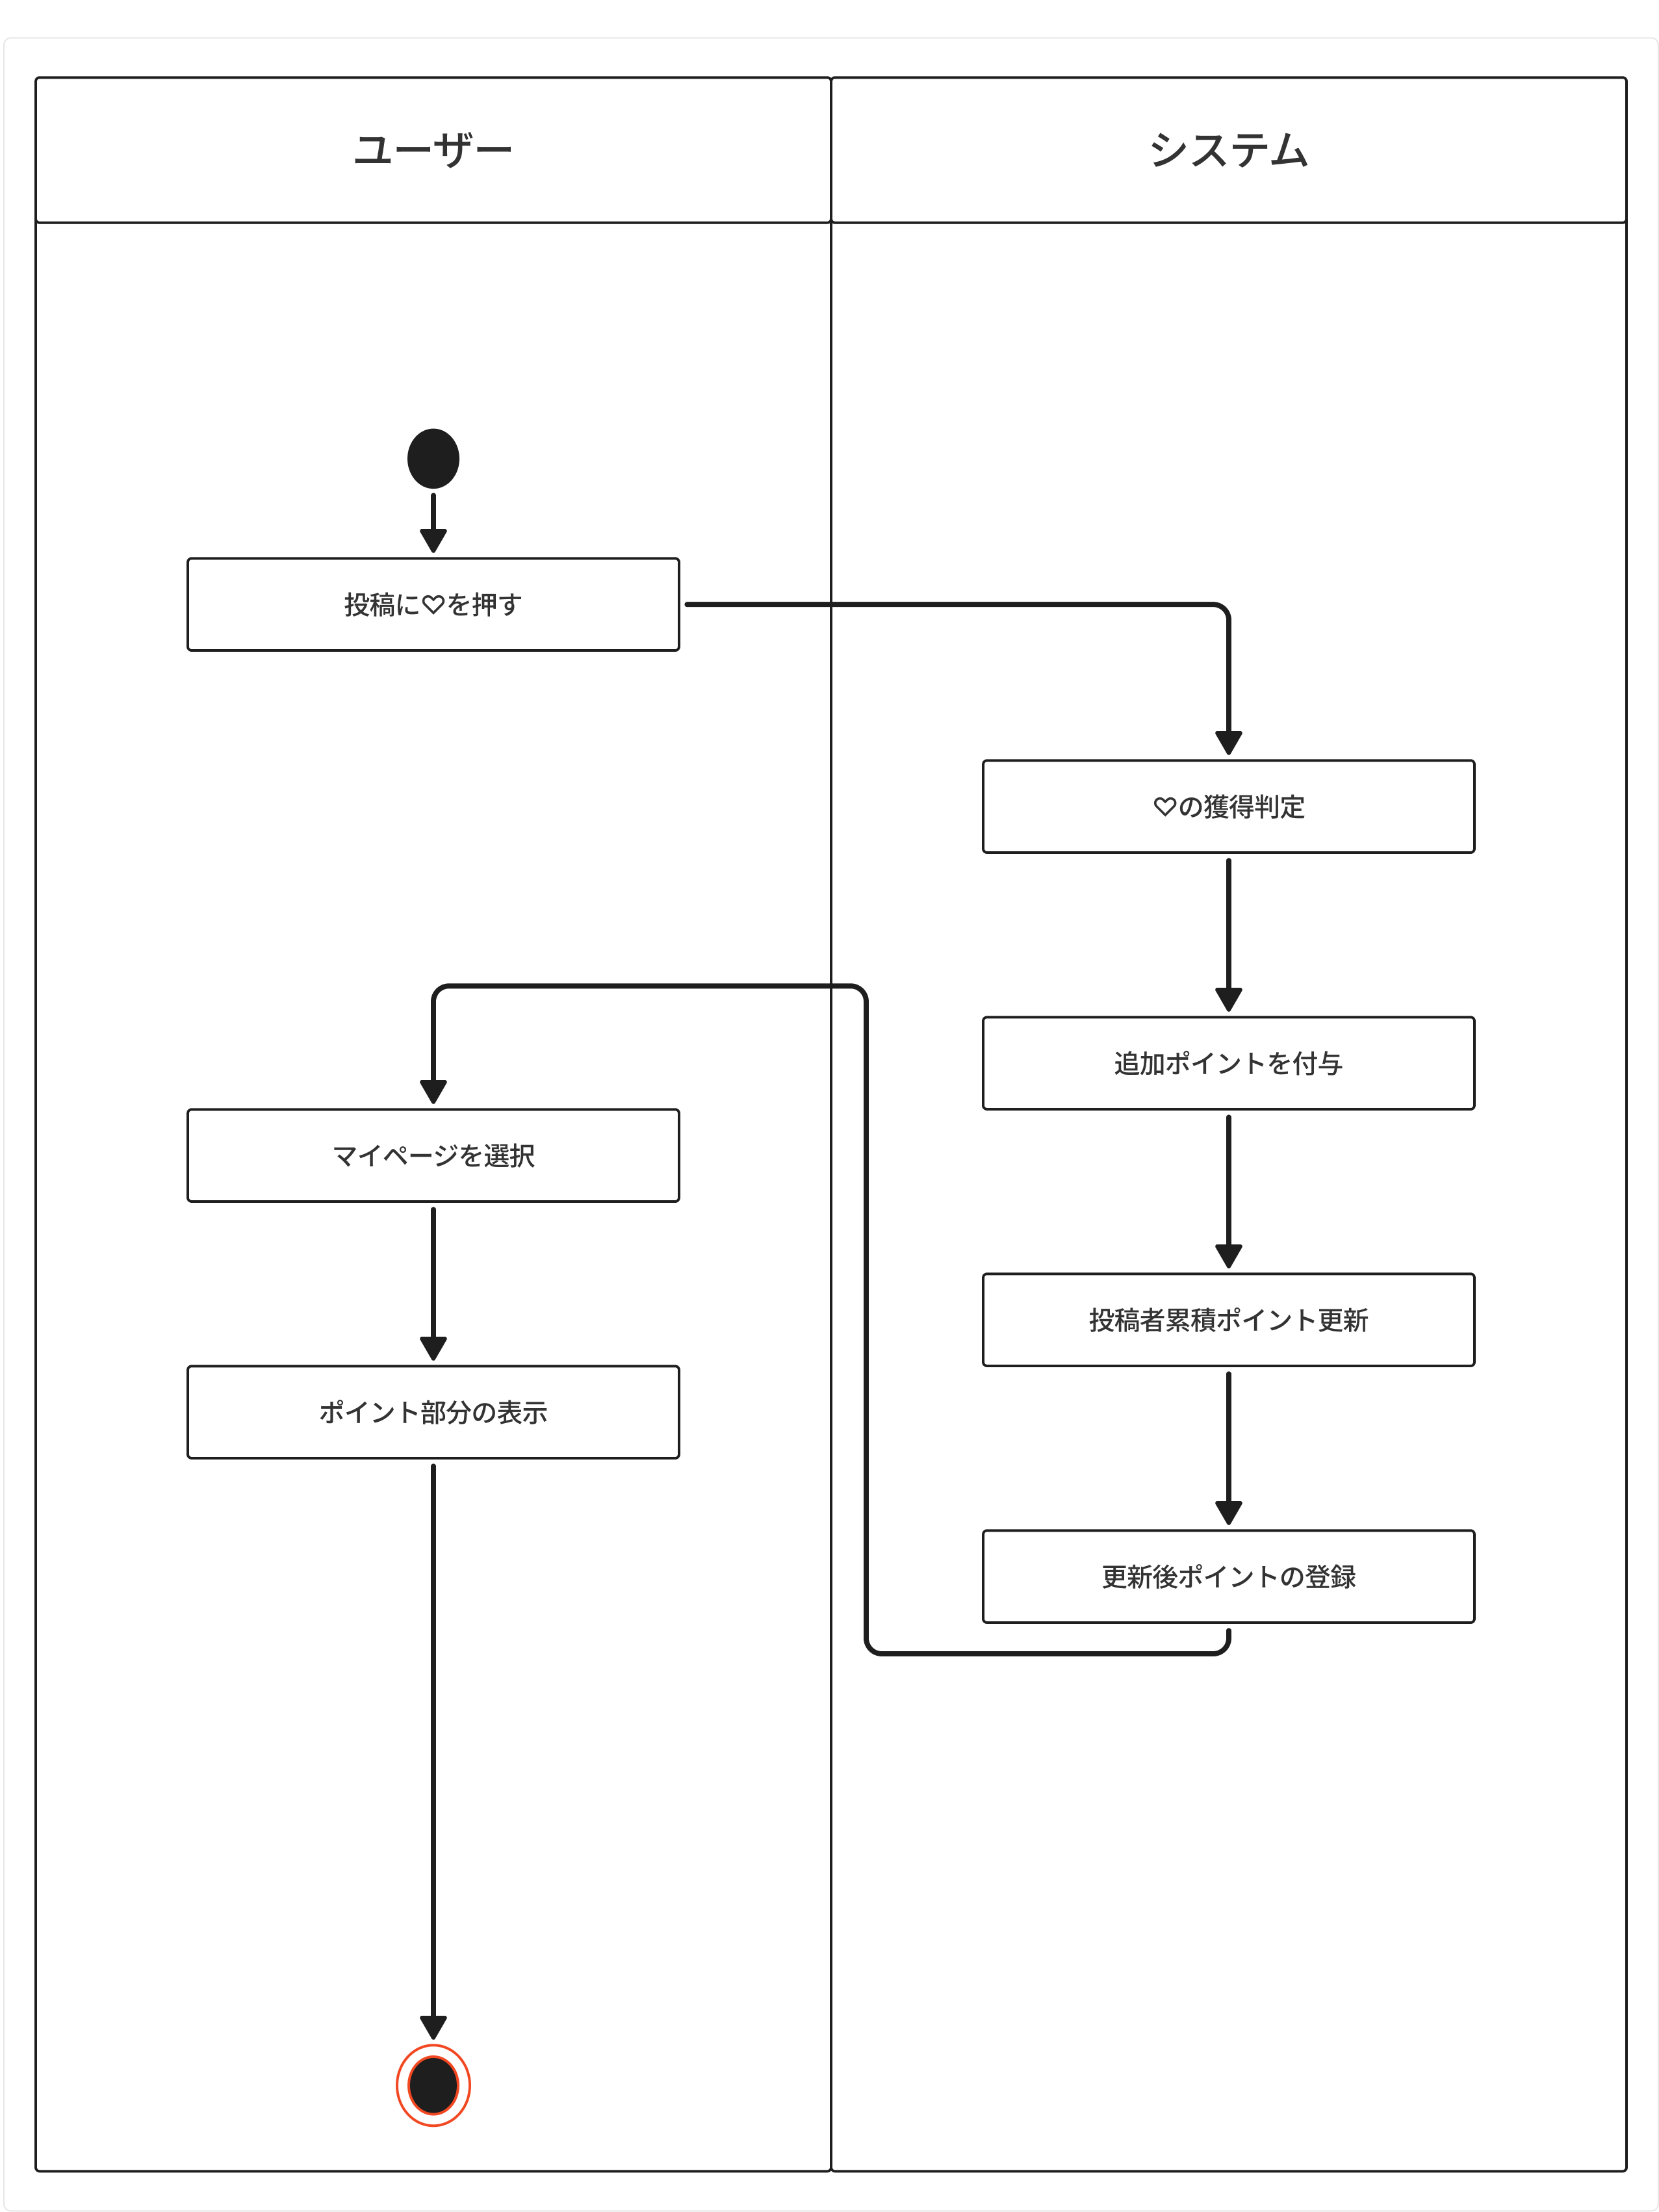
\includegraphics[width=0.5\textwidth]{chapters/images/n.png}
    \caption{ハートによるポイント付与機能}
\end{figure}
\subsubsection{設定機能}
本機能は、好みの画面設定・通知設定を反映される機能である。
\begin{figure}[H]
    \centering
    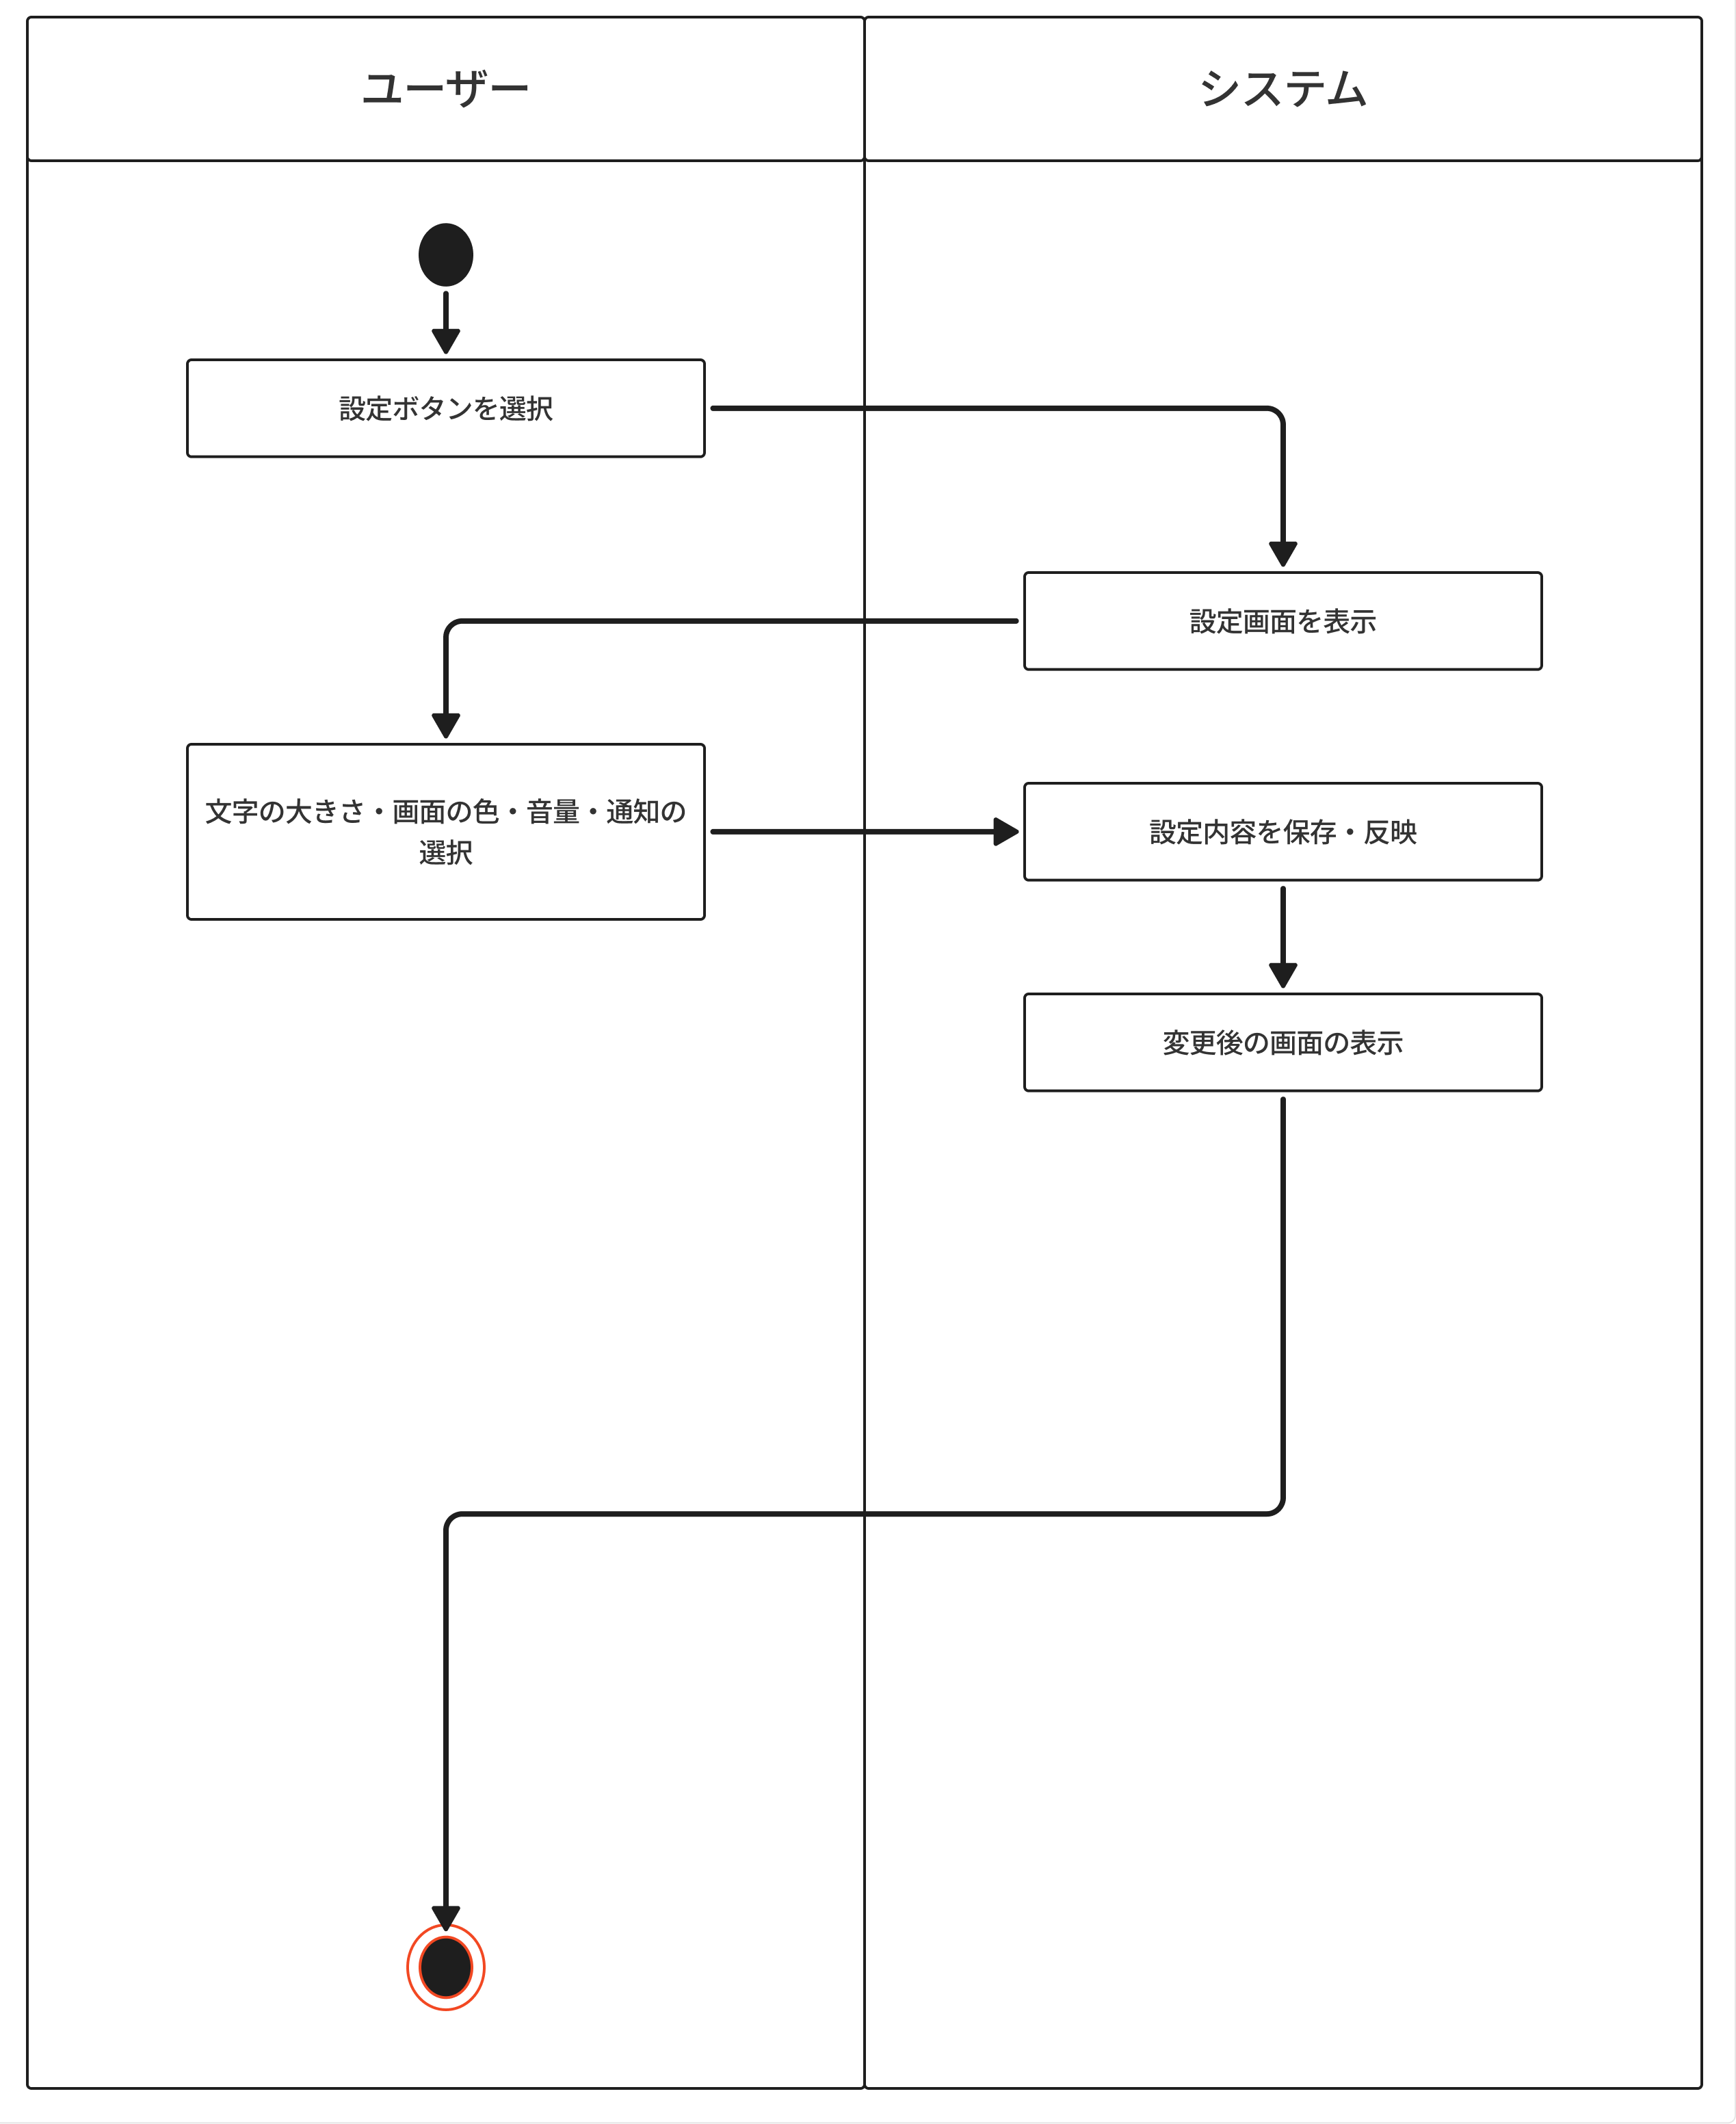
\includegraphics[width=0.5\textwidth]{chapters/images/o.png}
    \caption{設定機能}
\end{figure}
\subsubsection{チュートリアル機能}
本機能は、設定機能に含まれており、チュートリアルを再度表示し情報を確認できる機能である。アプリを最初に使用する際にチュートリアルを表示するが、もう一度確認したい場合に選択する。
\begin{figure}[H]
    \centering
    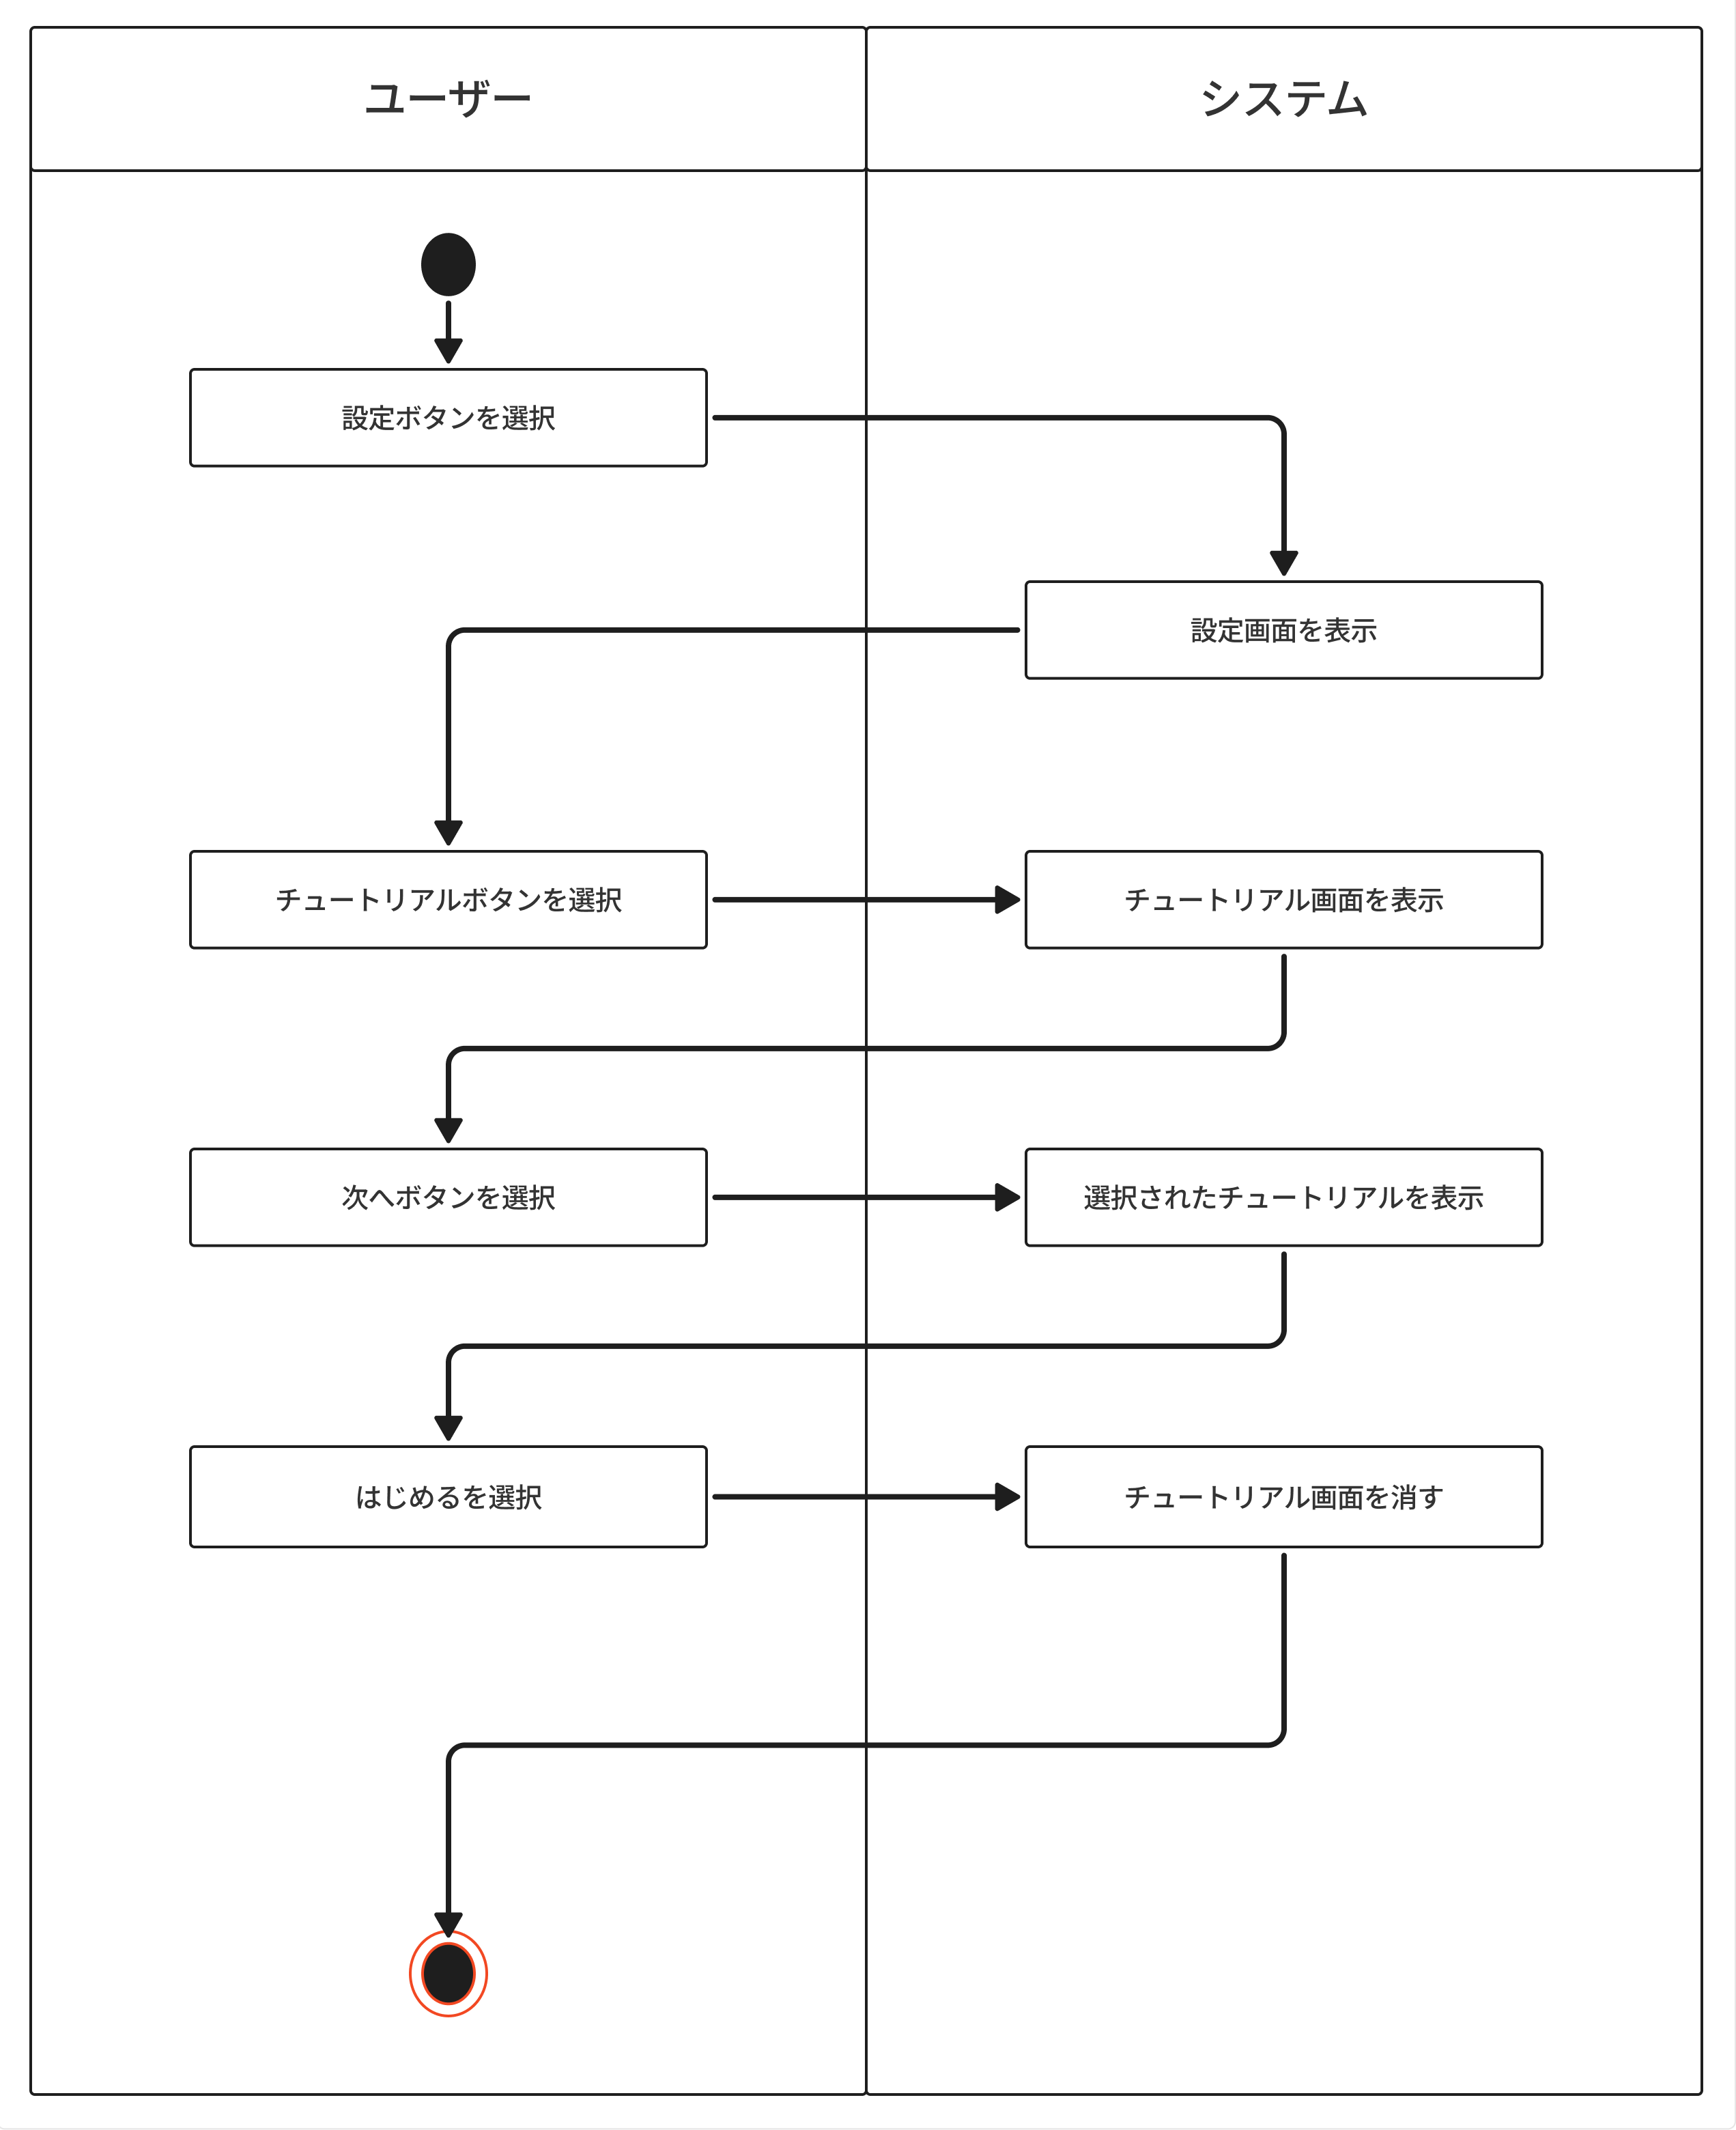
\includegraphics[width=0.5\textwidth]{chapters/images/p.png}
    \caption{チュートリアル機能}
\end{figure}
\subsubsection{バージョン表示機能}
本機能は、設定機能に含まれており、アプリケーションのバージョンを確認できる機能
\begin{figure}[H]
    \centering
    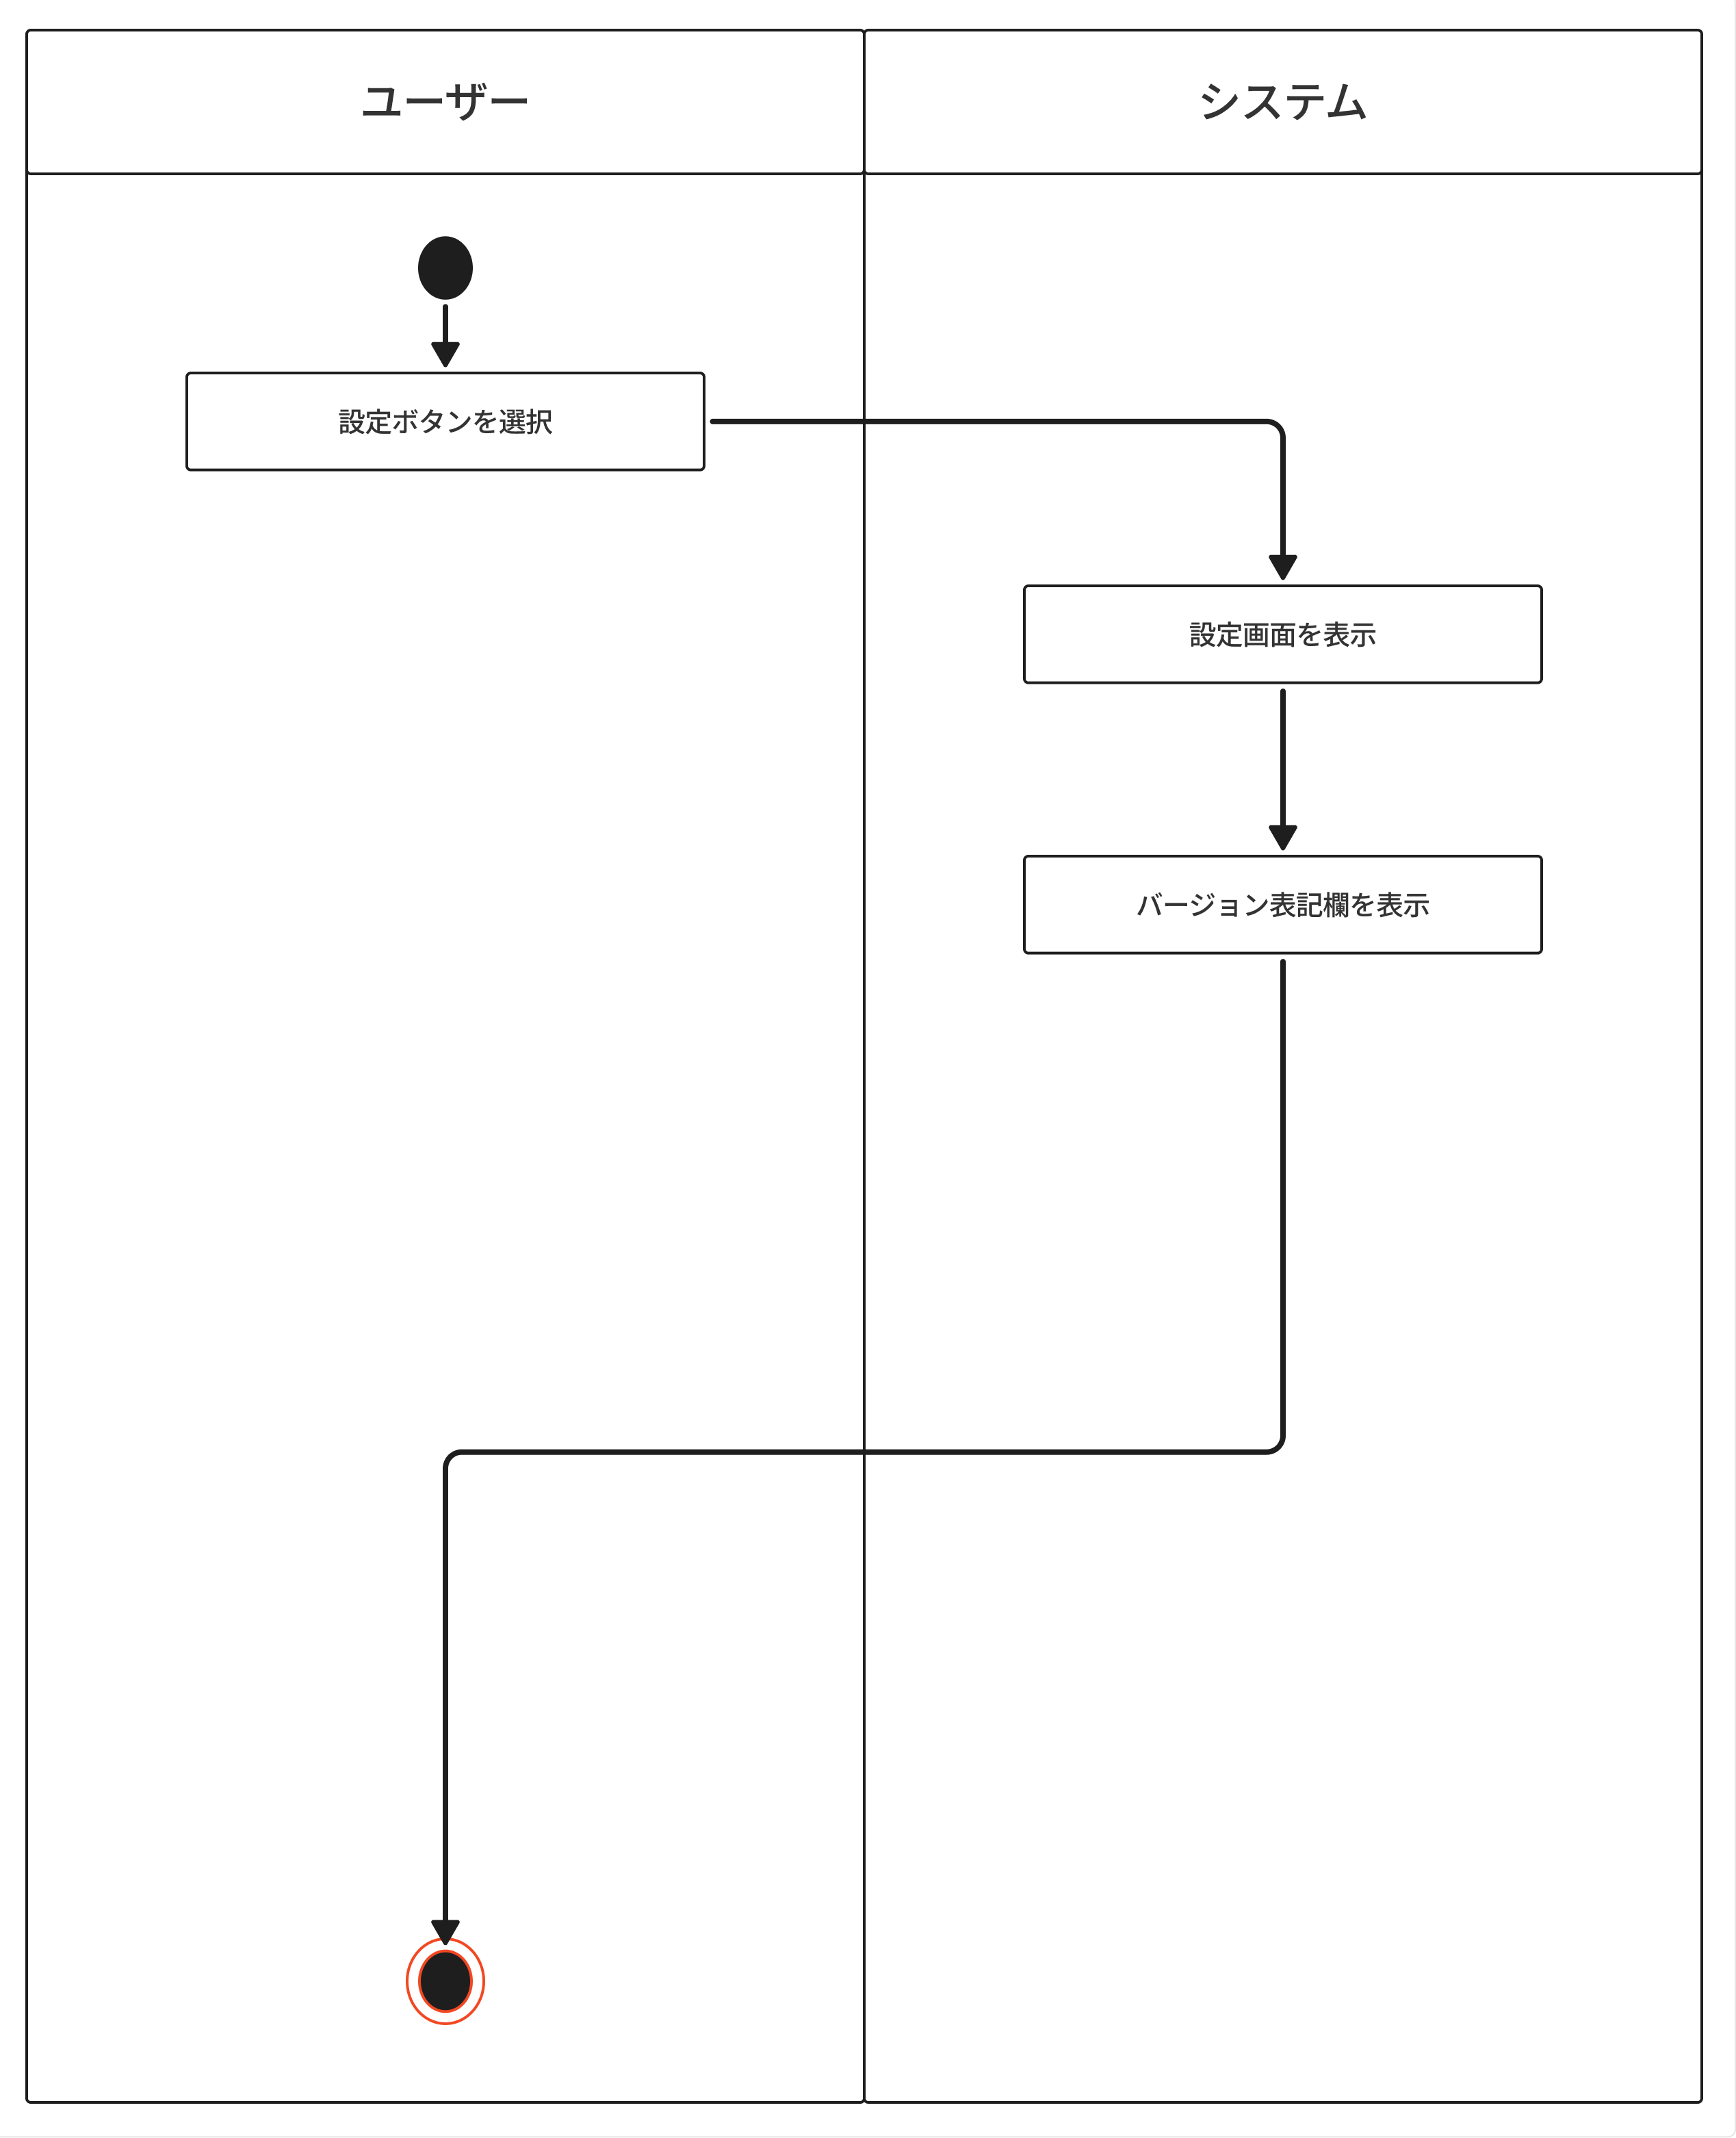
\includegraphics[width=0.5\textwidth]{chapters/images/q.png}
    \caption{バージョン表示機能}
\end{figure}
\subsubsection{お知らせ機能}
本機能は、お知らせ機能はアプリのお知らせメッセージや投稿に対する質問が届いたことを通知するメッセージやスマホ教室を告知するメッセージを受信ボックスのように一覧に表示する機能
\begin{figure}[H]
    \centering
    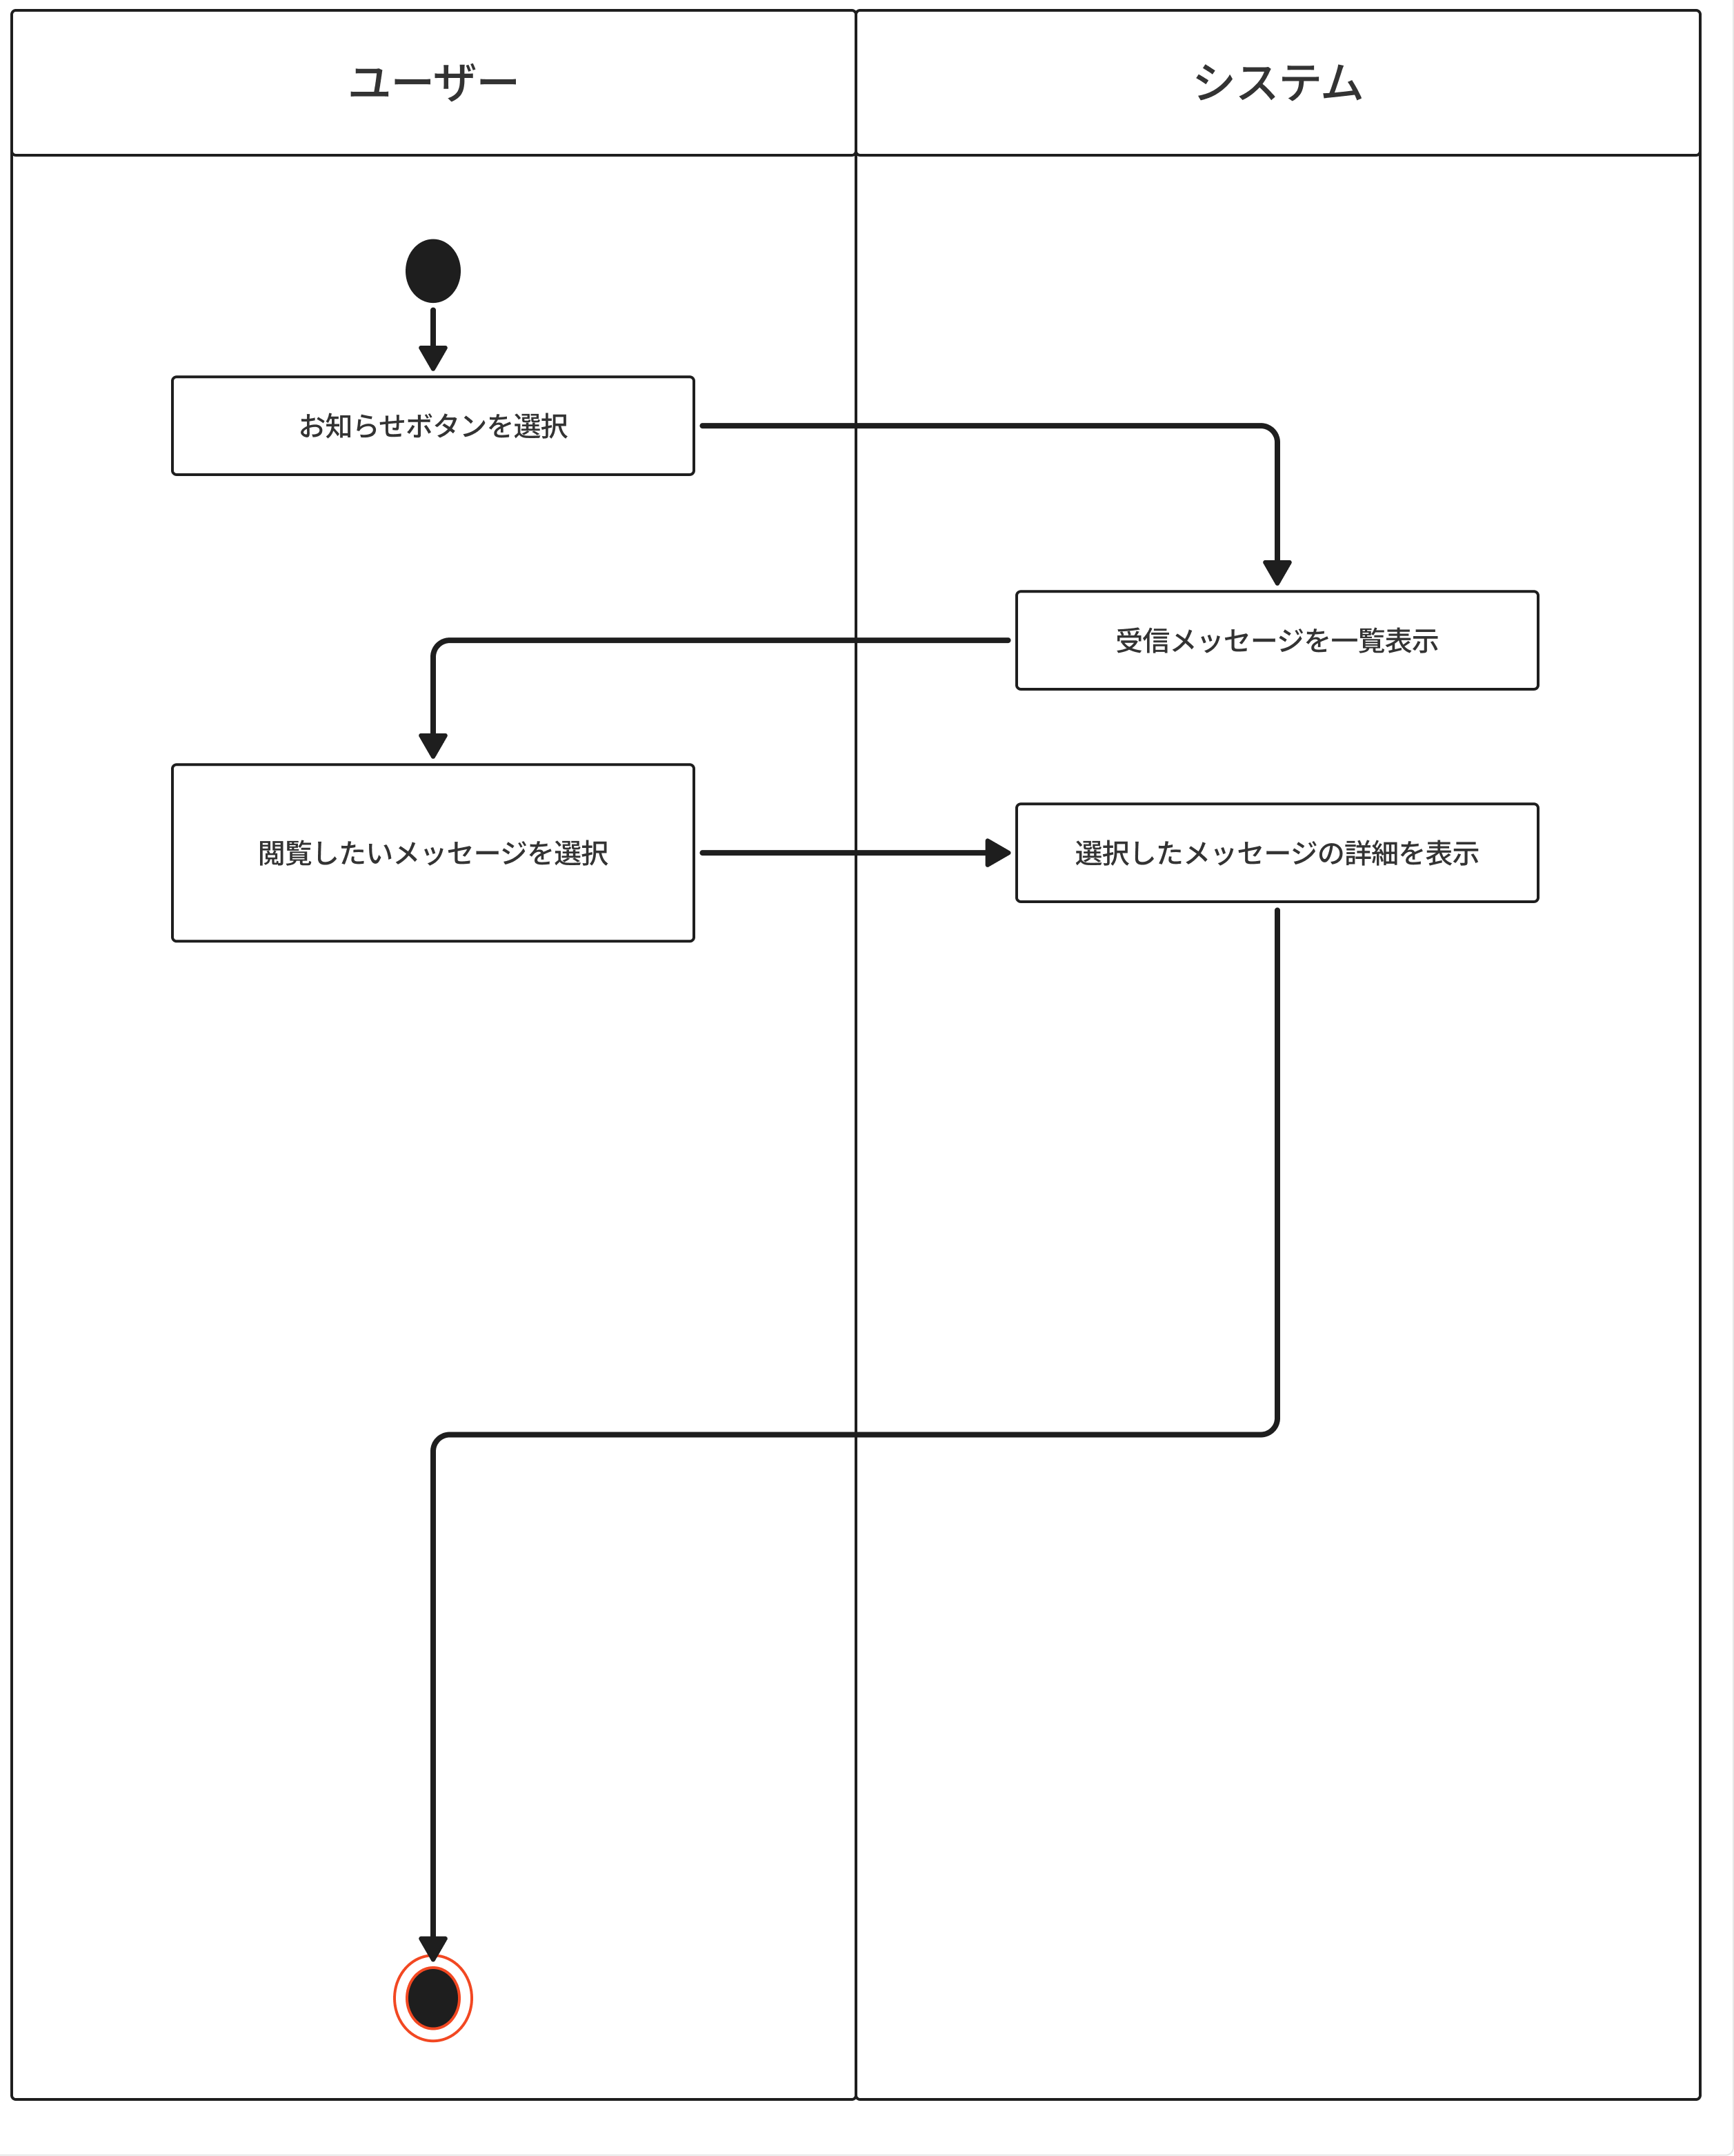
\includegraphics[width=0.5\textwidth]{chapters/images/r.png}
    \caption{お知らせ機能}
\end{figure}
\subsubsection{お問合せ機能}
本機能は、本アプリ内でわからないことを直接管理者に聞ける機能である。実際にメッセージとして飛ばすことで絶対的な解決を目指す。
\begin{figure}[H]
    \centering
    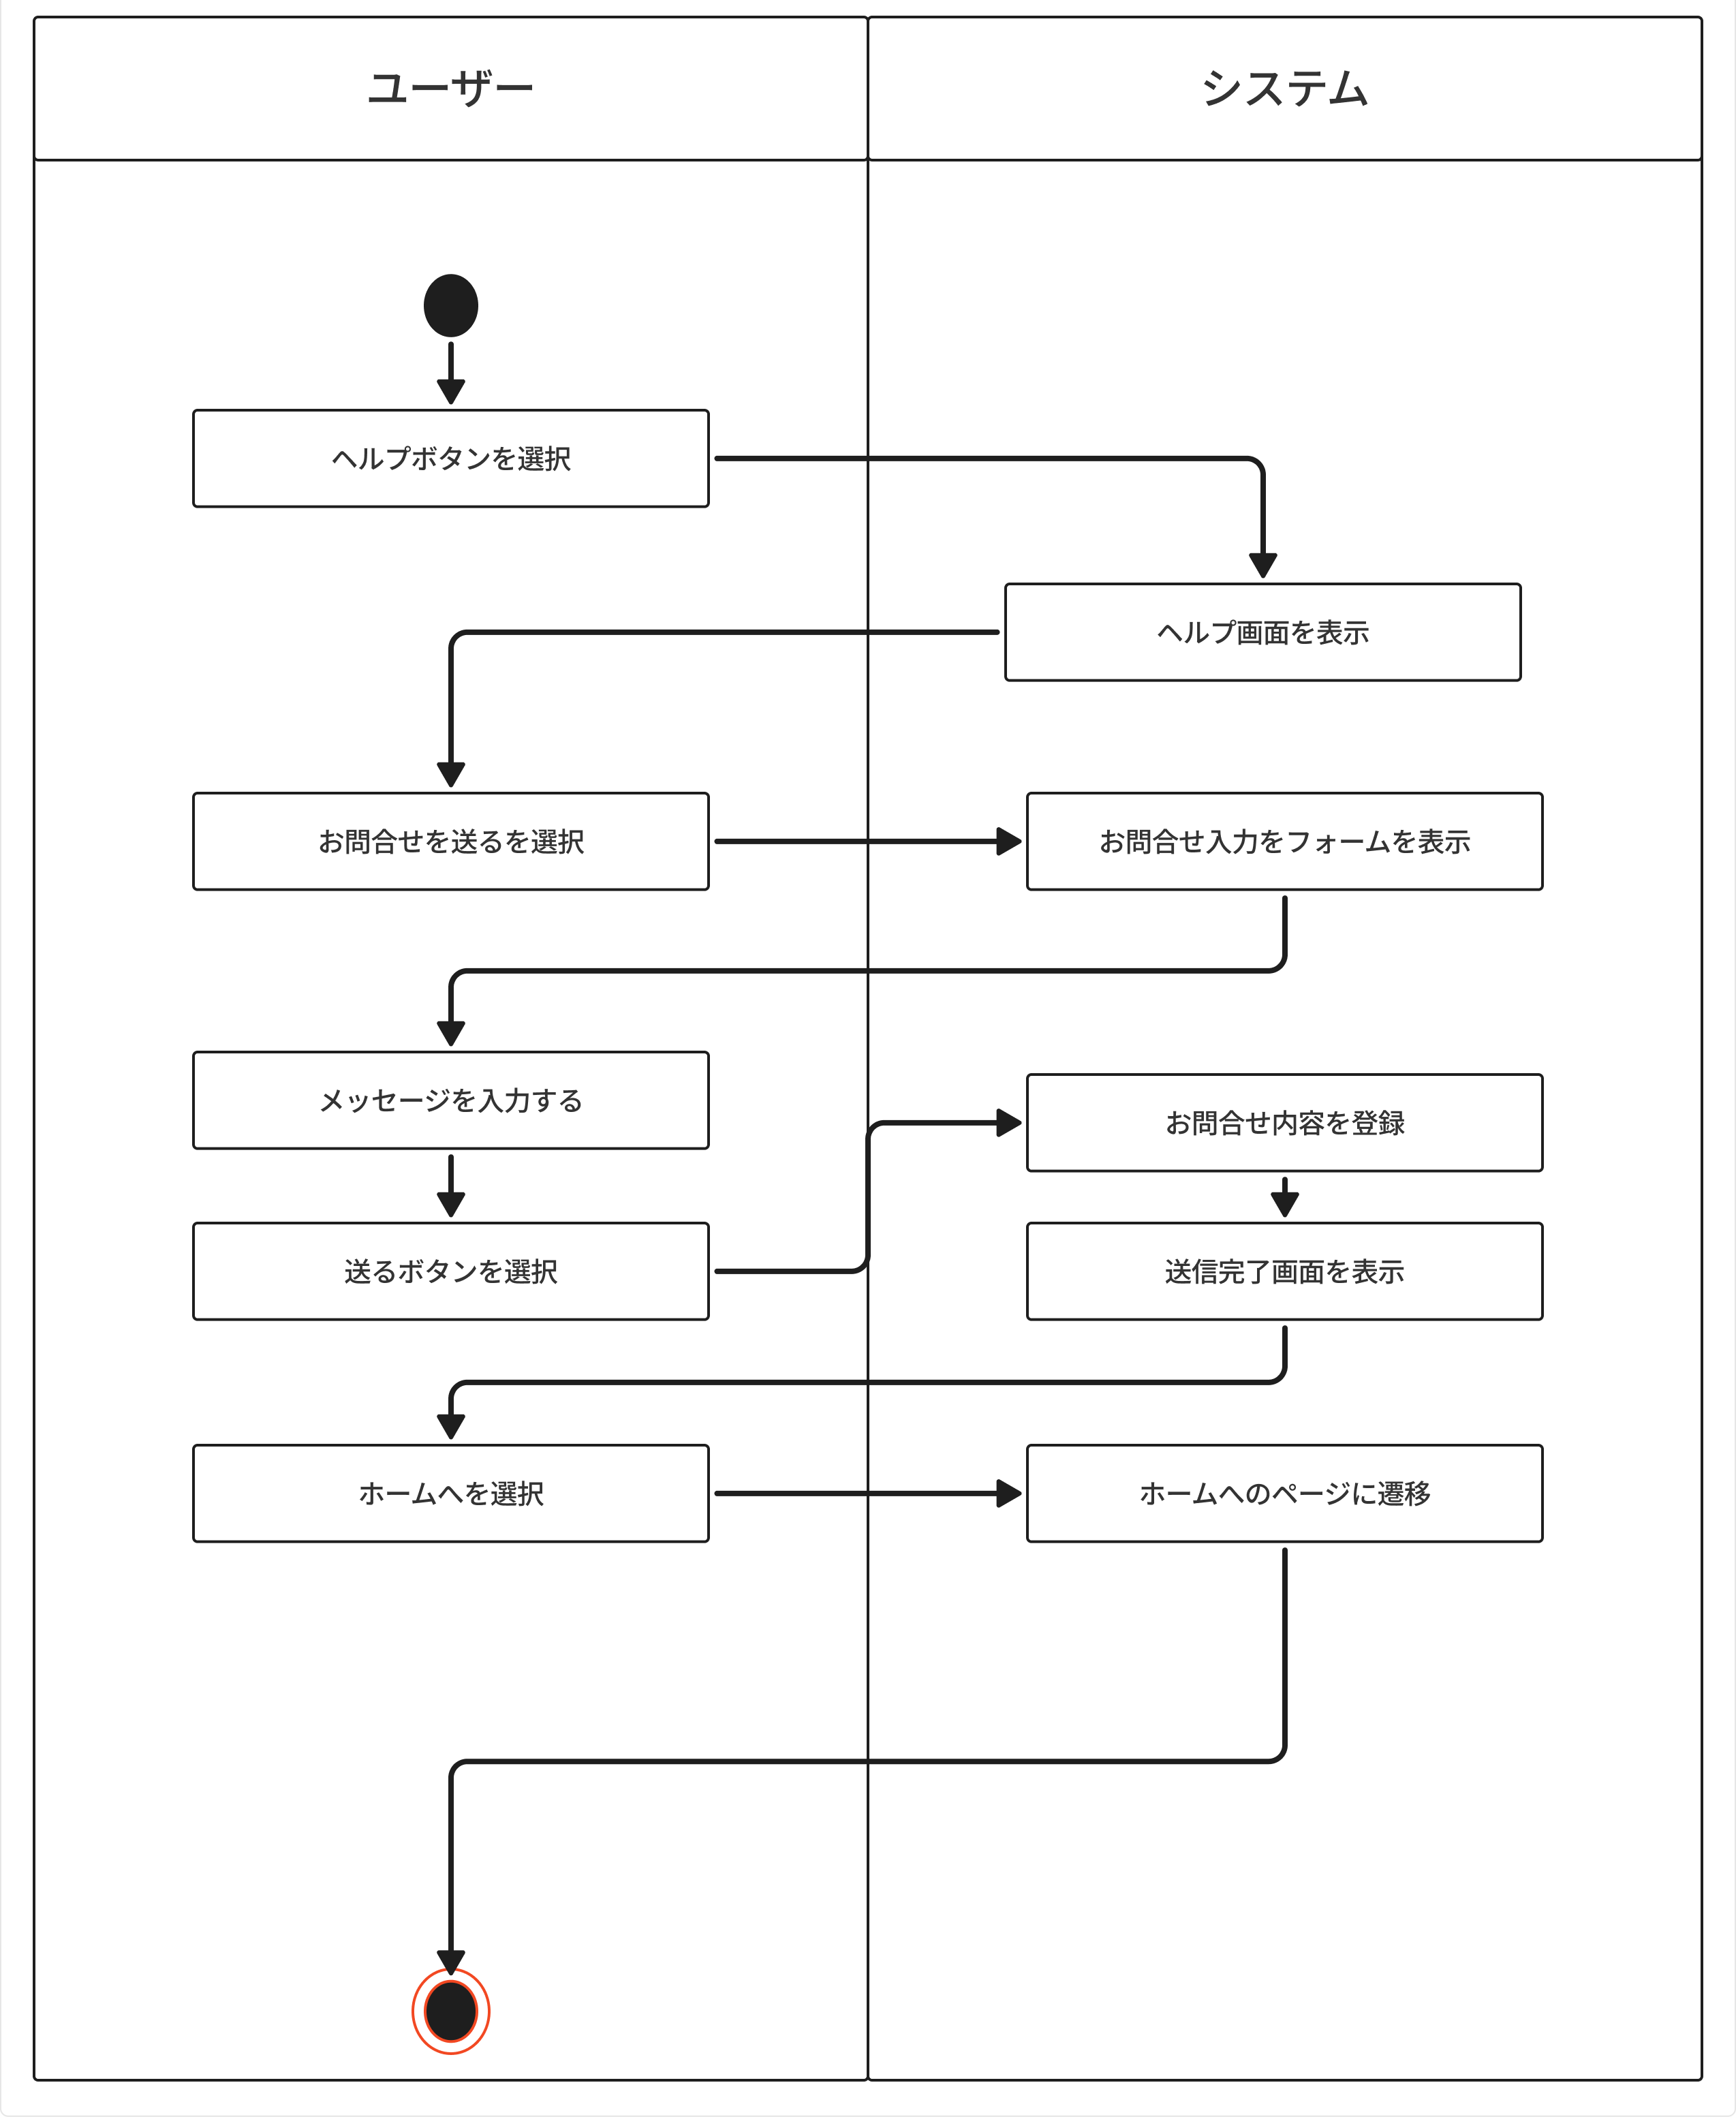
\includegraphics[width=0.5\textwidth]{chapters/images/s.png}
    \caption{お問合せ機能}
\end{figure}



\subsection{管理者}

\subsubsection{ユーザー管理機能}
本機能は、システムに登録されたユーザーの一覧確認やアカウントの状態管理、権限変更を行う機能である。
\begin{figure}[H]
    \centering
    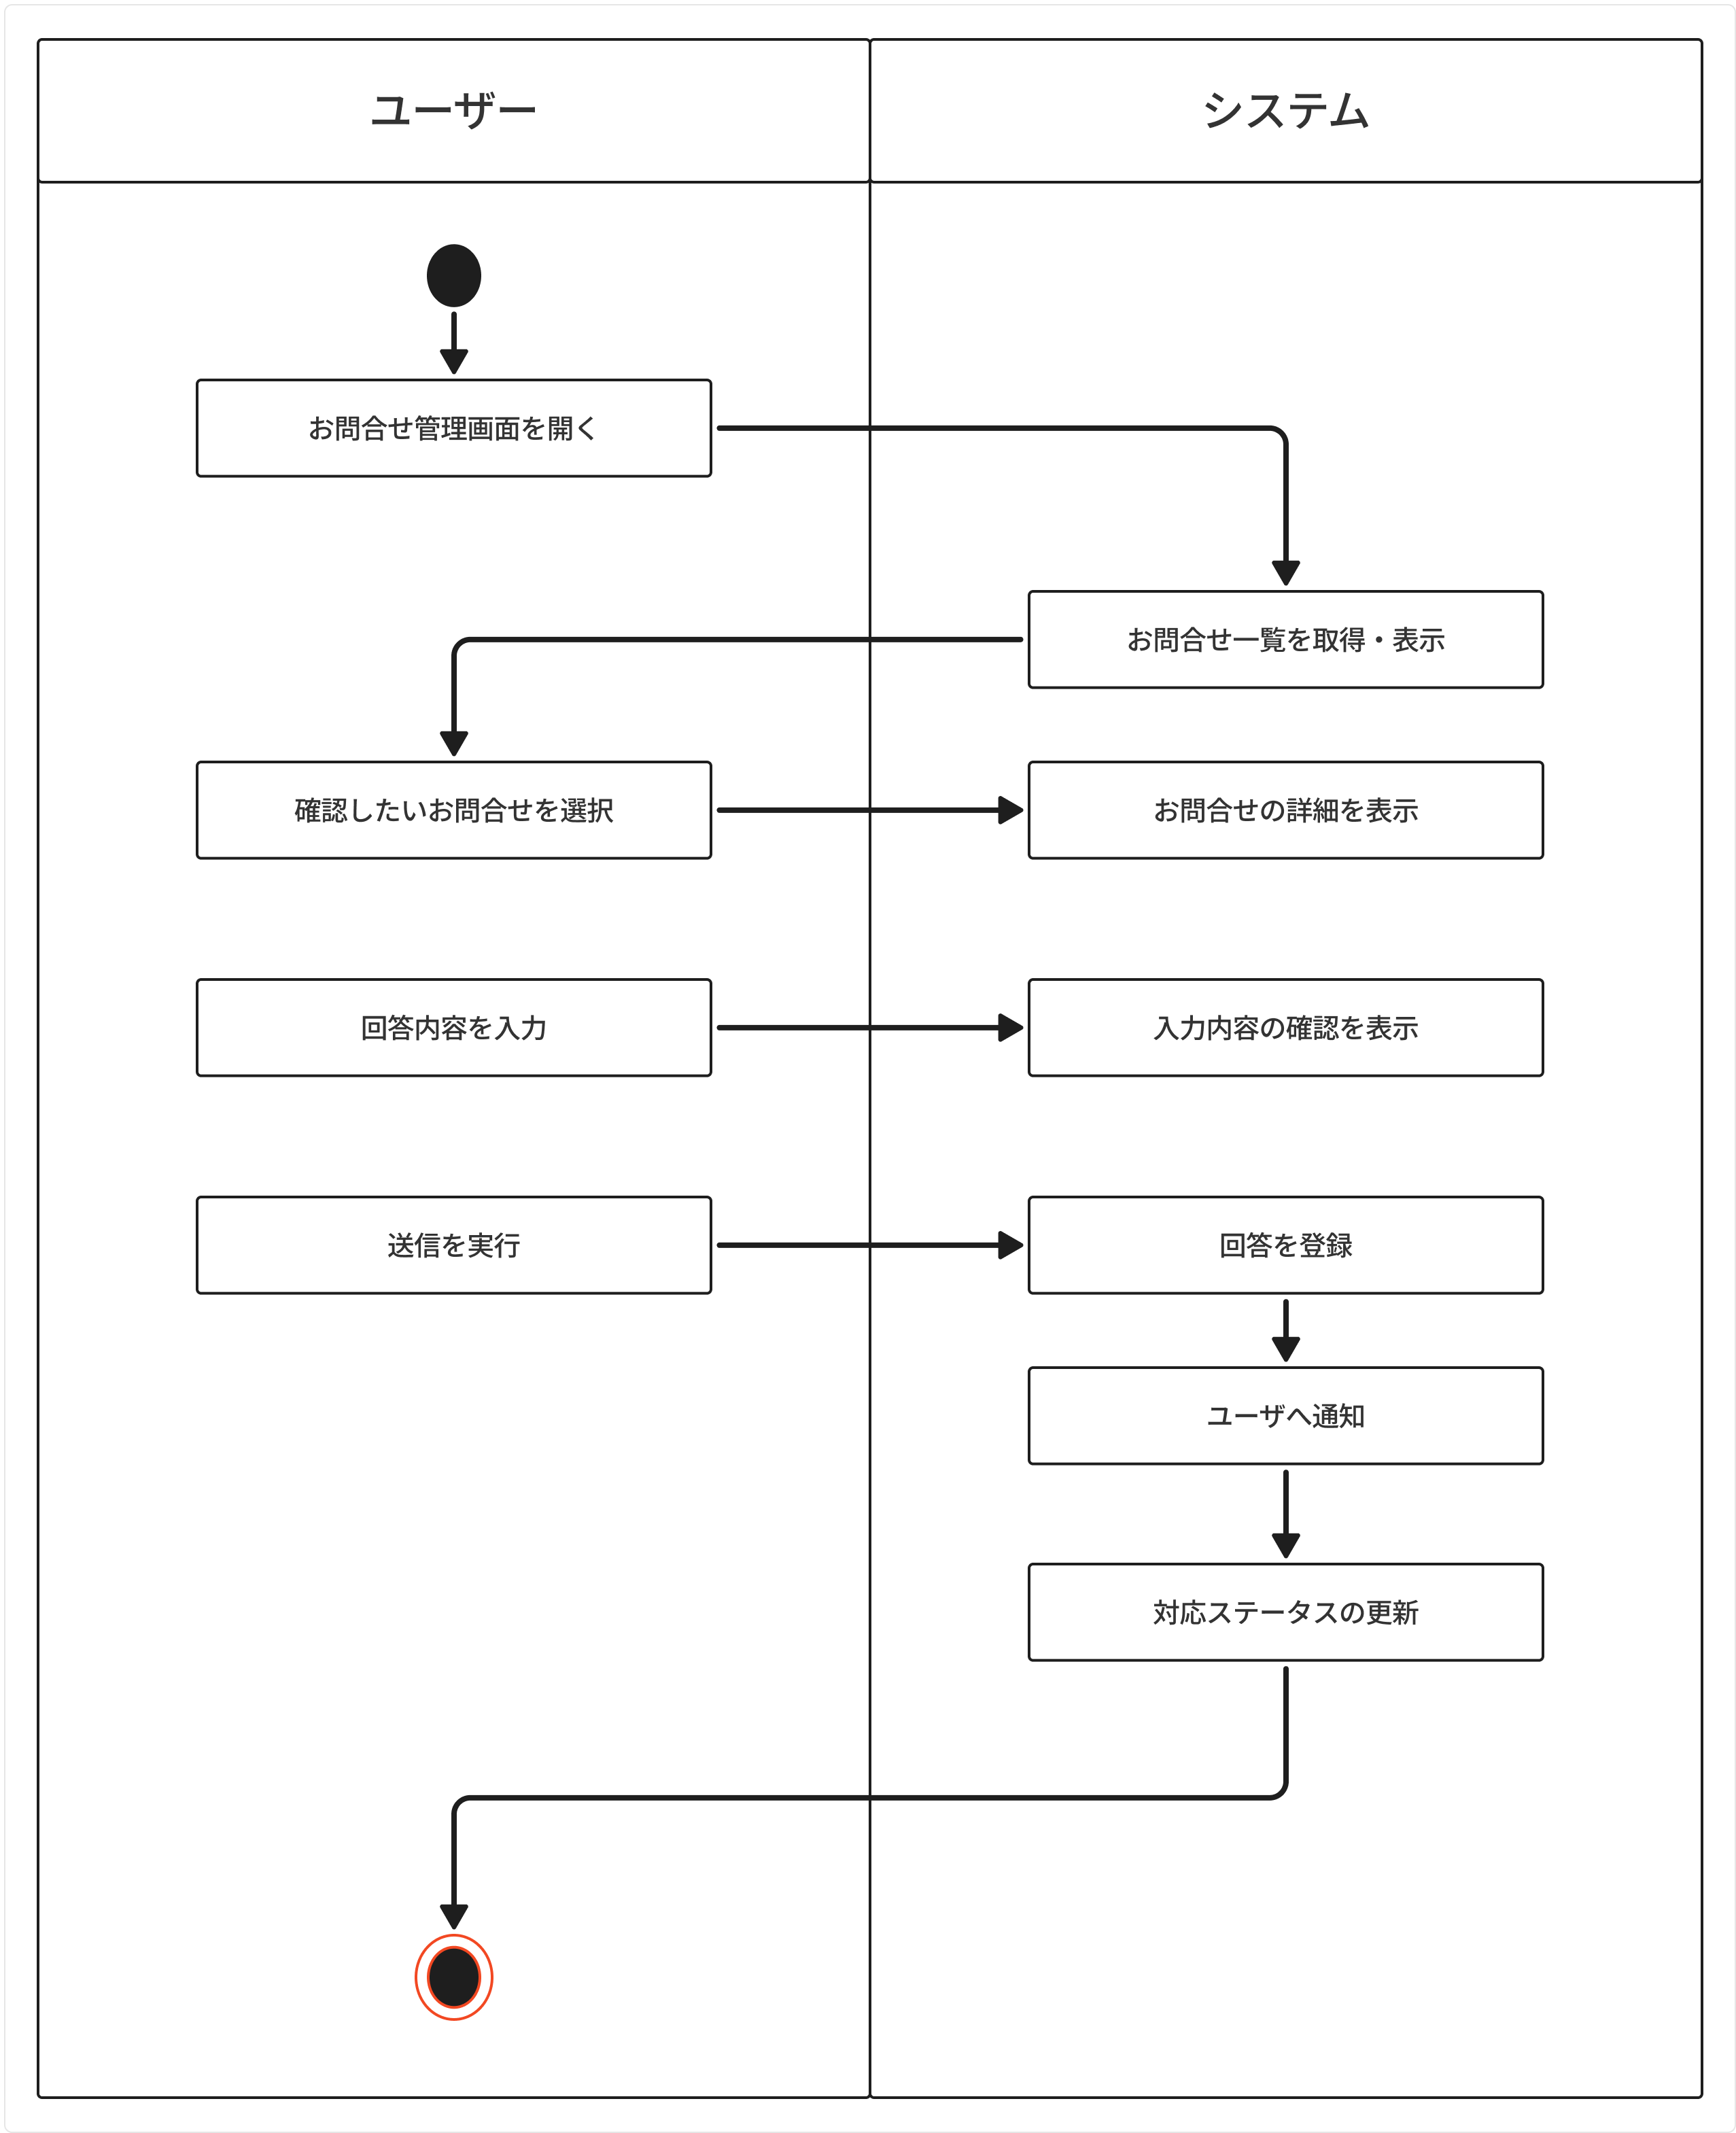
\includegraphics[width=0.5\textwidth]{chapters/images/t.png}
    \caption{ユーザー管理機能}
\end{figure}

\subsubsection{投稿・コンテンツ管理機能}
本機能は、ユーザーから投稿されたコンテンツの内容を確認し、不適切な投稿の確認や削除などの管理を行う機能である。
\begin{figure}[H]
    \centering
    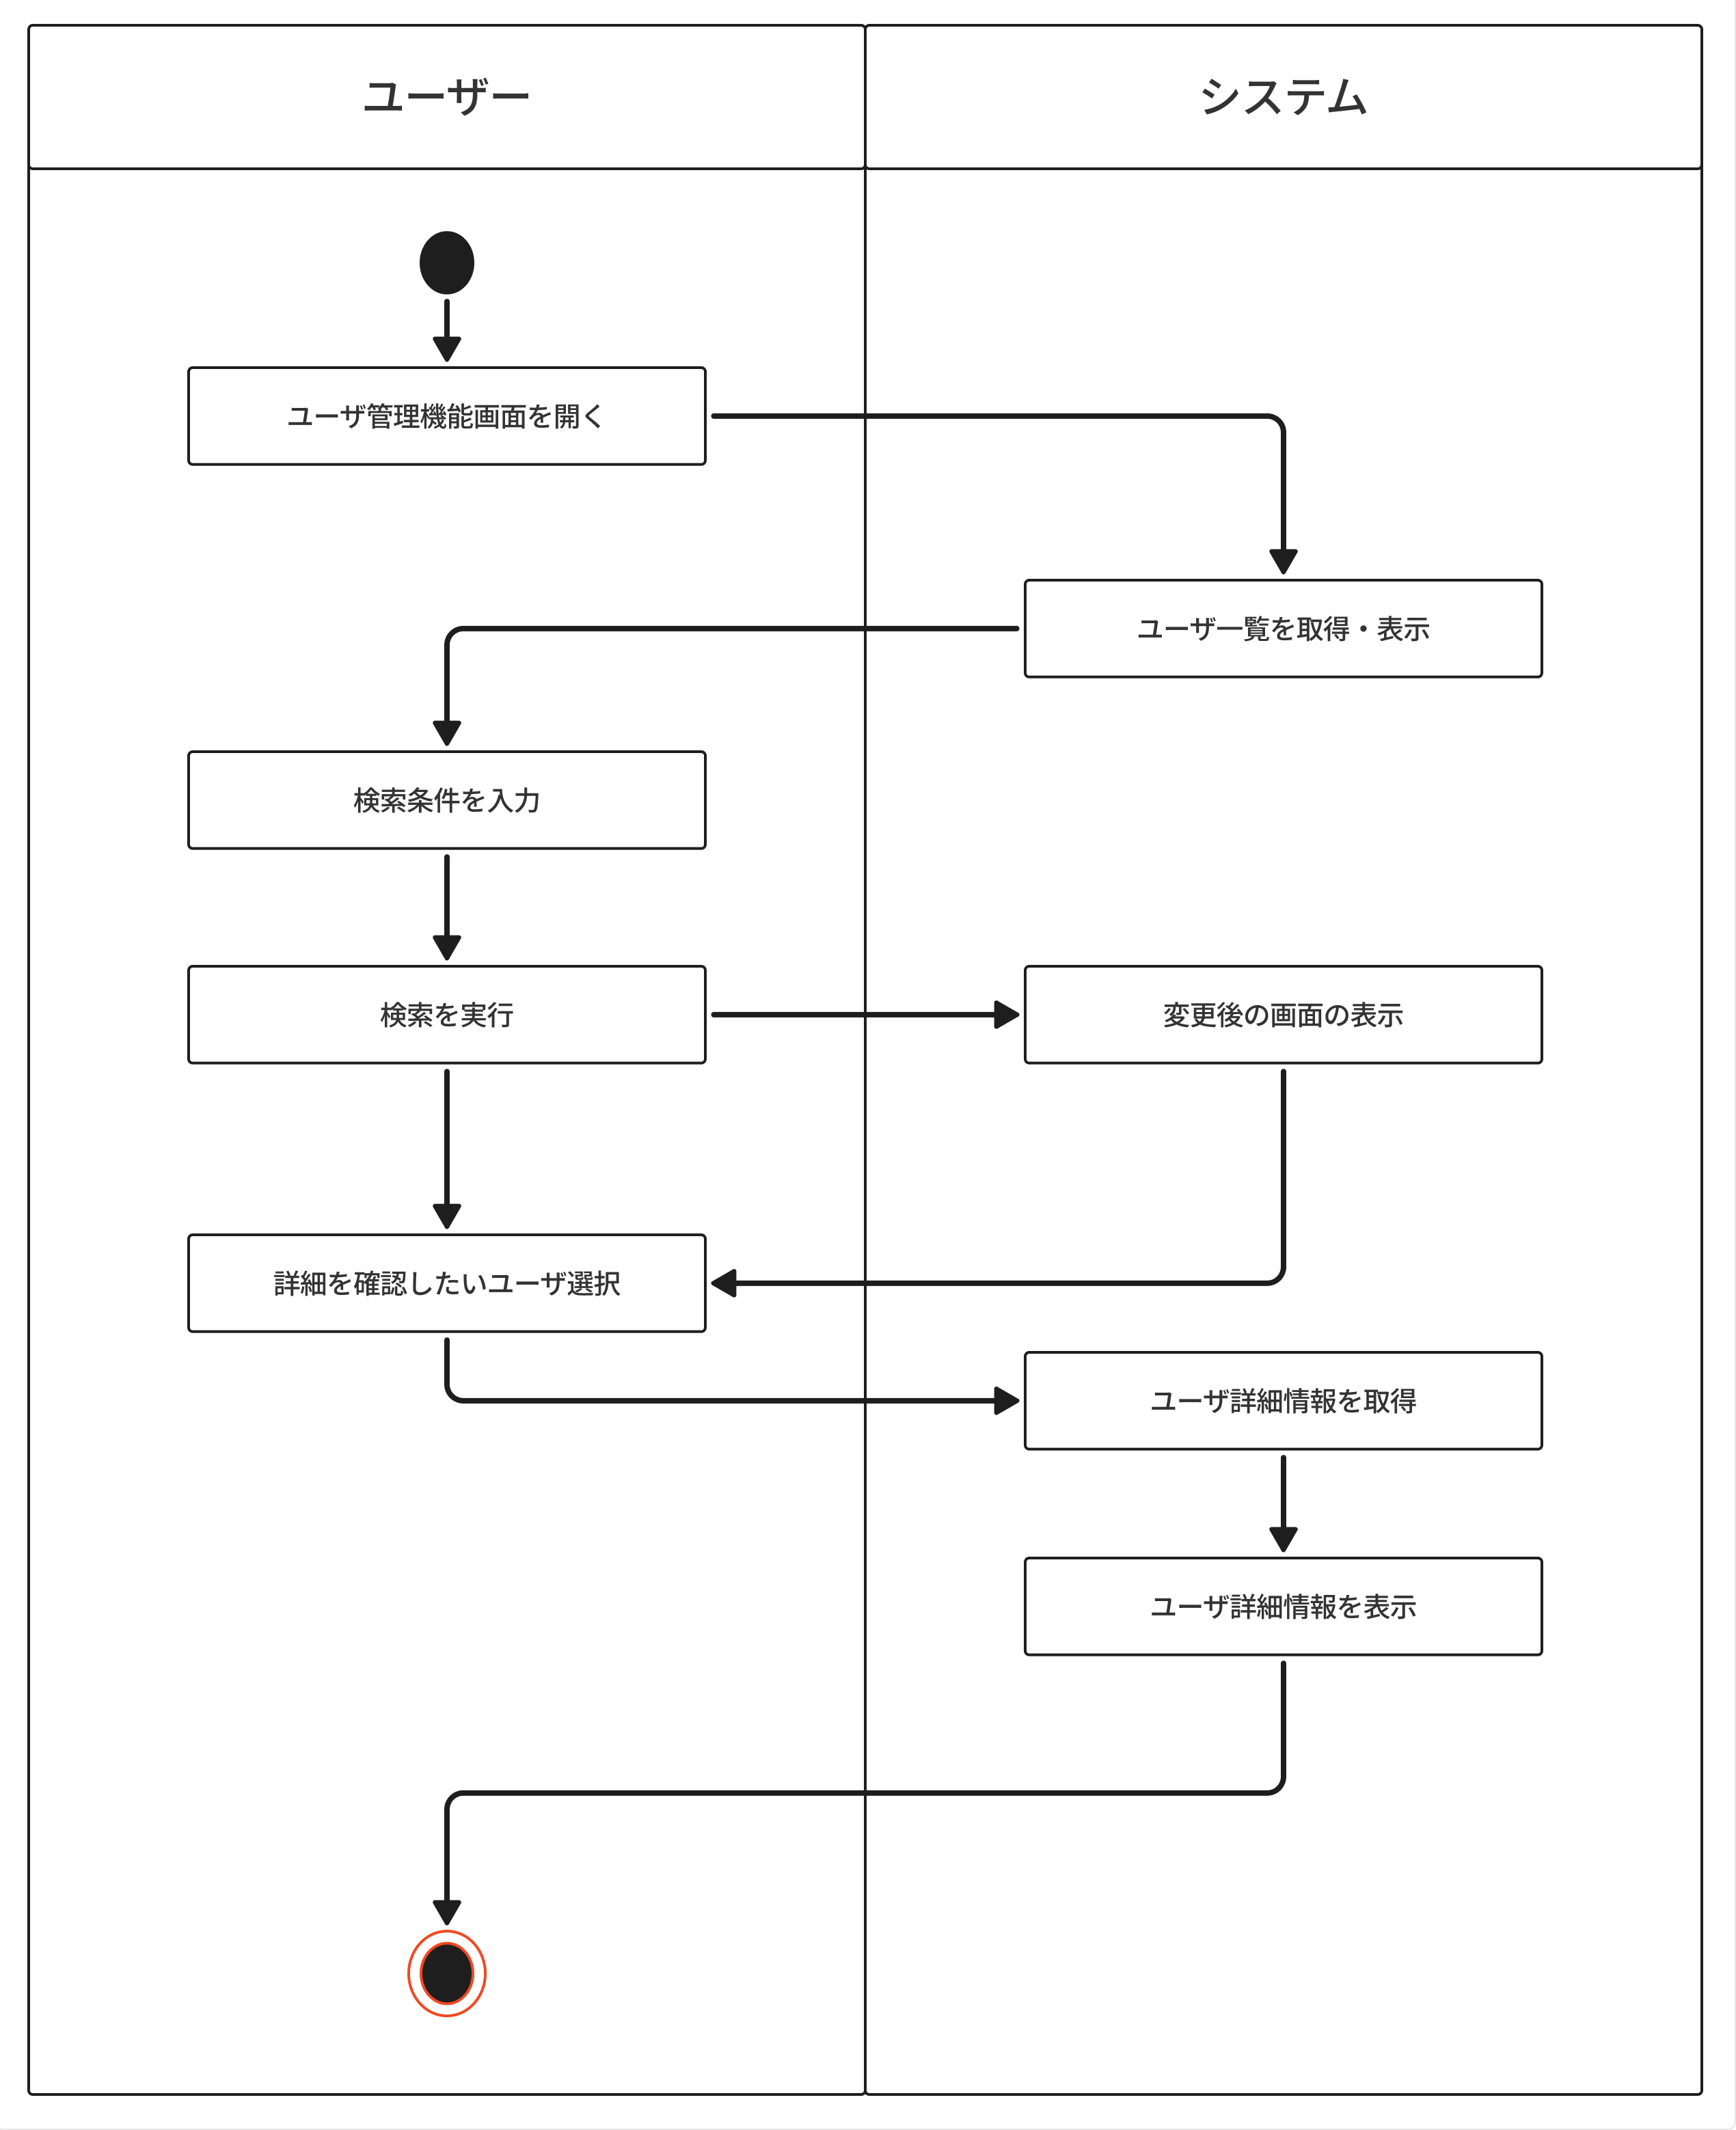
\includegraphics[width=0.5\textwidth]{chapters/images/u.png}
    \caption{投稿・コンテンツ管理機能}
\end{figure}

\subsubsection{問い合わせ管理機能}
本機能は、ユーザーから送信されたお問合せ内容を確認し、管理者として個別に対応や返信を行う機能である。
\begin{figure}[H]
    \centering
    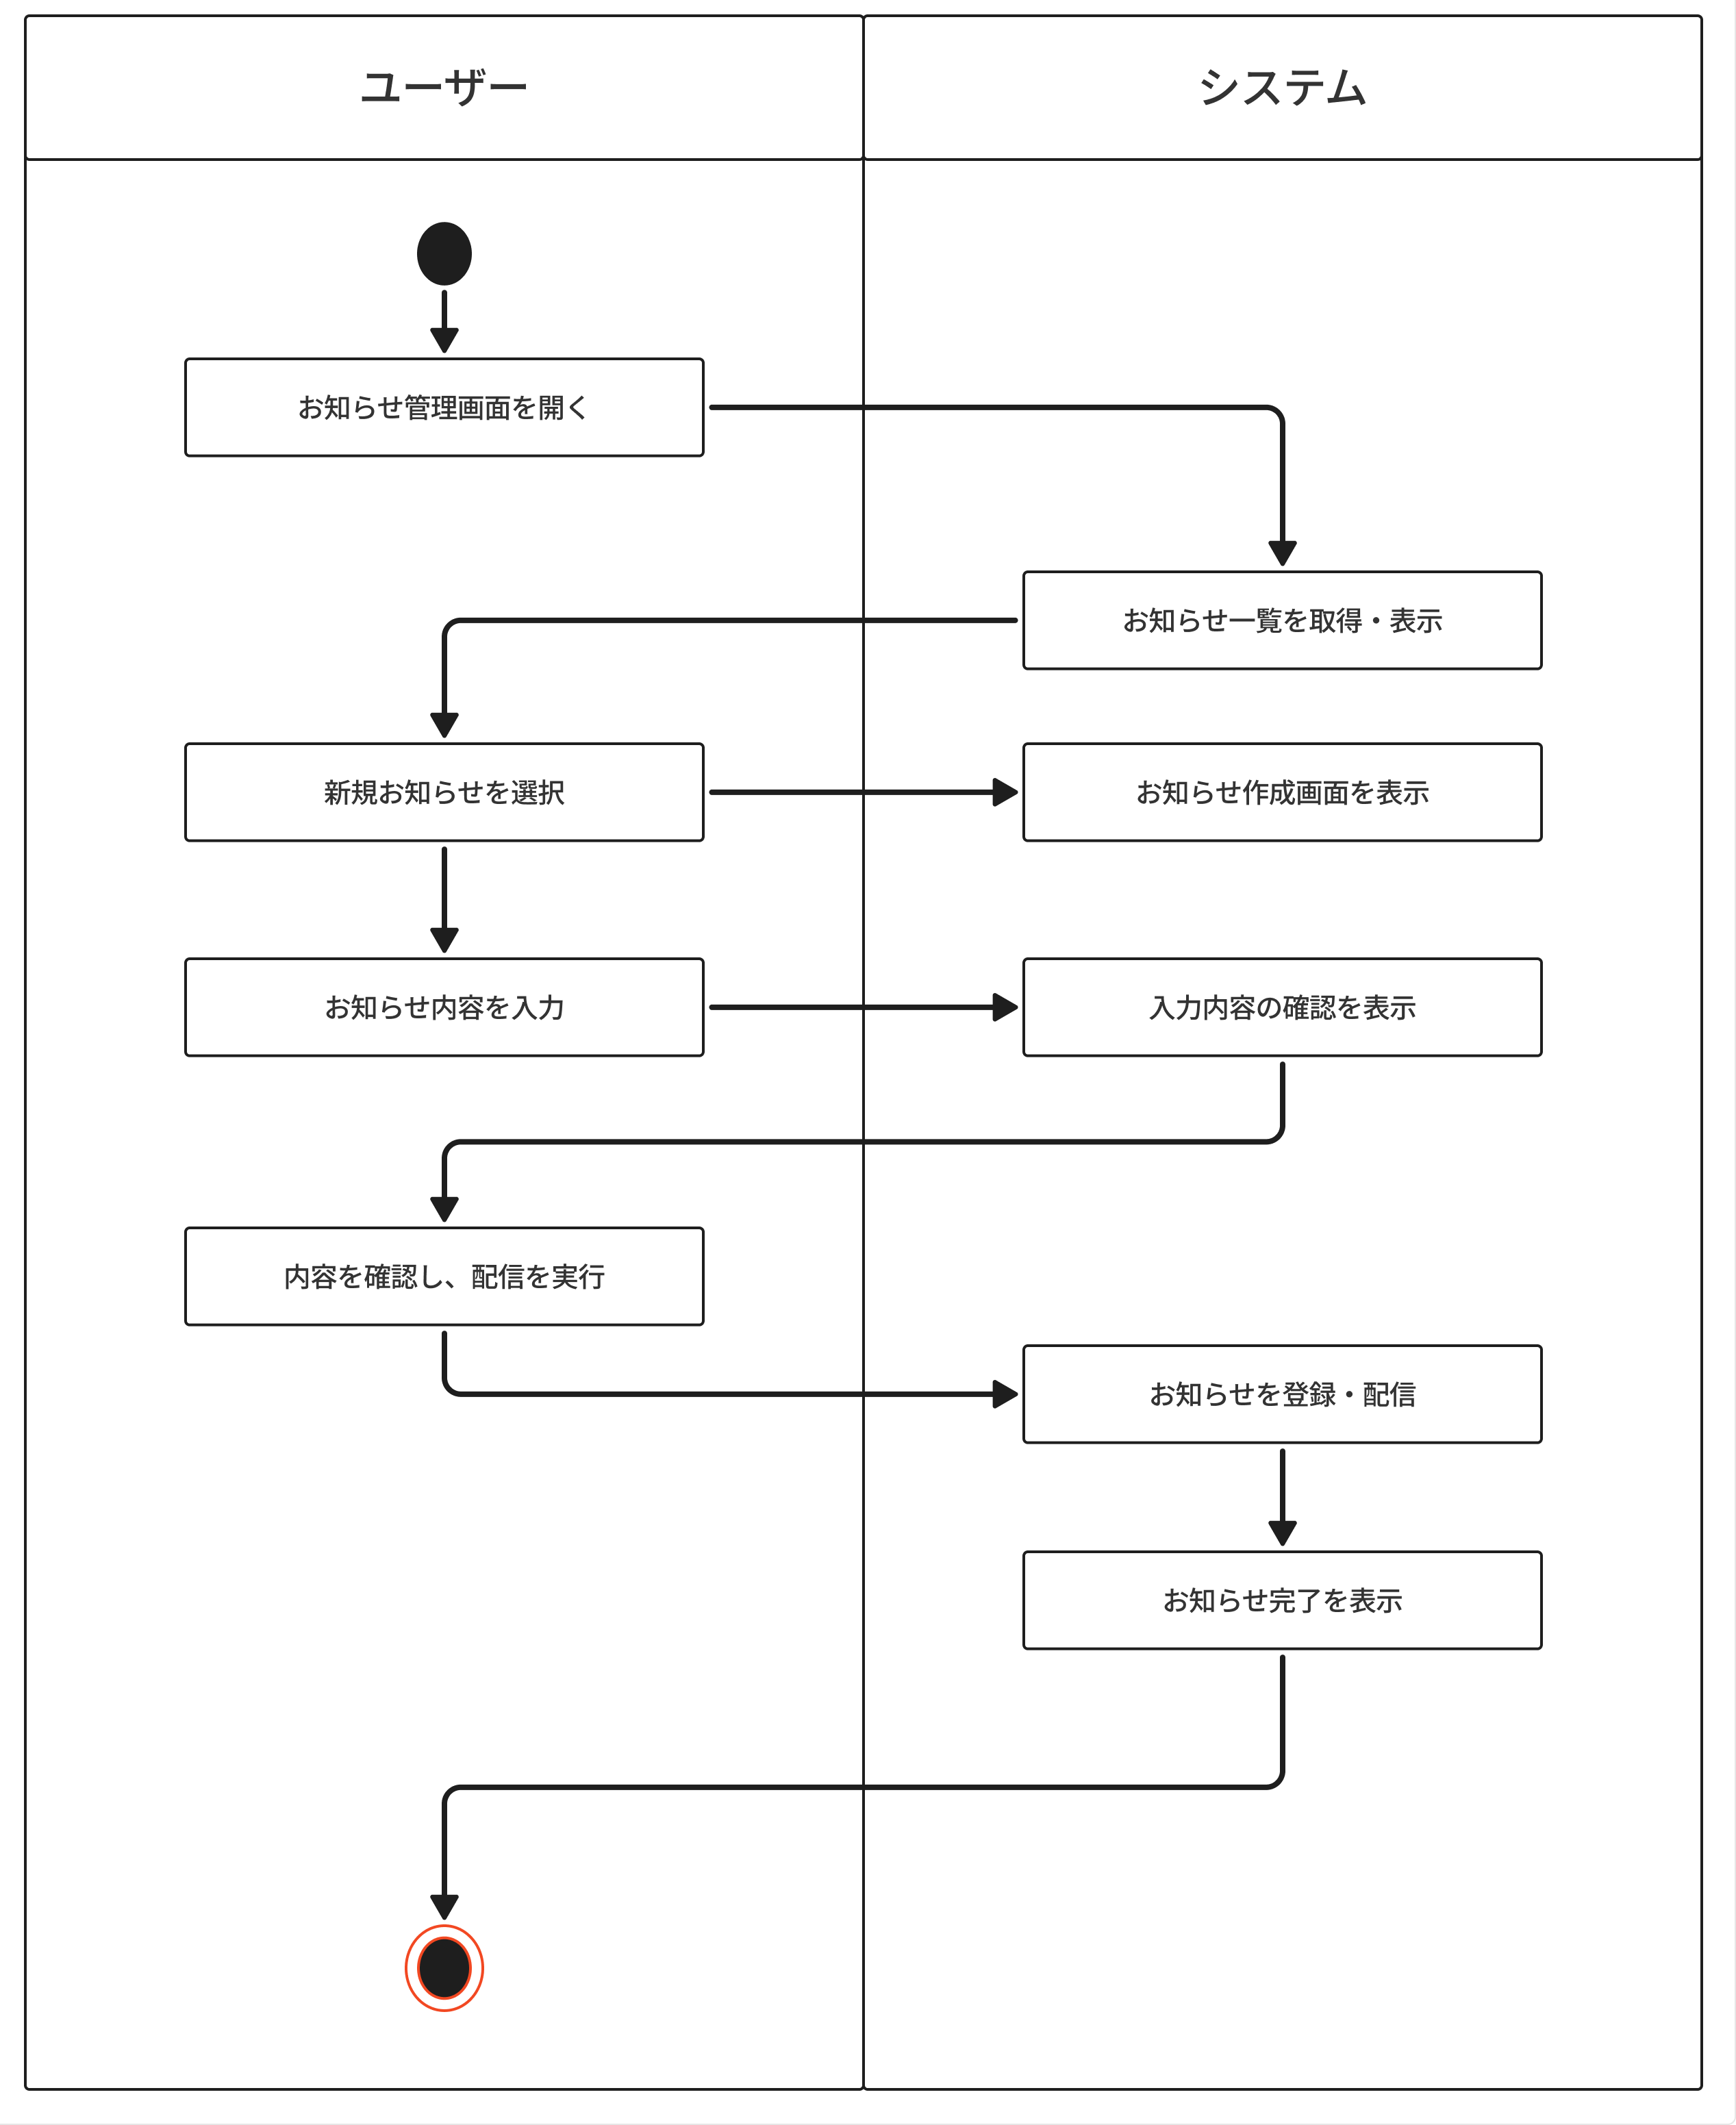
\includegraphics[width=0.5\textwidth]{chapters/images/v.png}
    \caption{問い合わせ管理機能}
\end{figure}

\subsubsection{お知らせ配信機能}
本機能は、アプリ全体のお知らせやイベント情報を作成し、ユーザーに向けて配信・管理する機能である。
\begin{figure}[H]
    \centering
    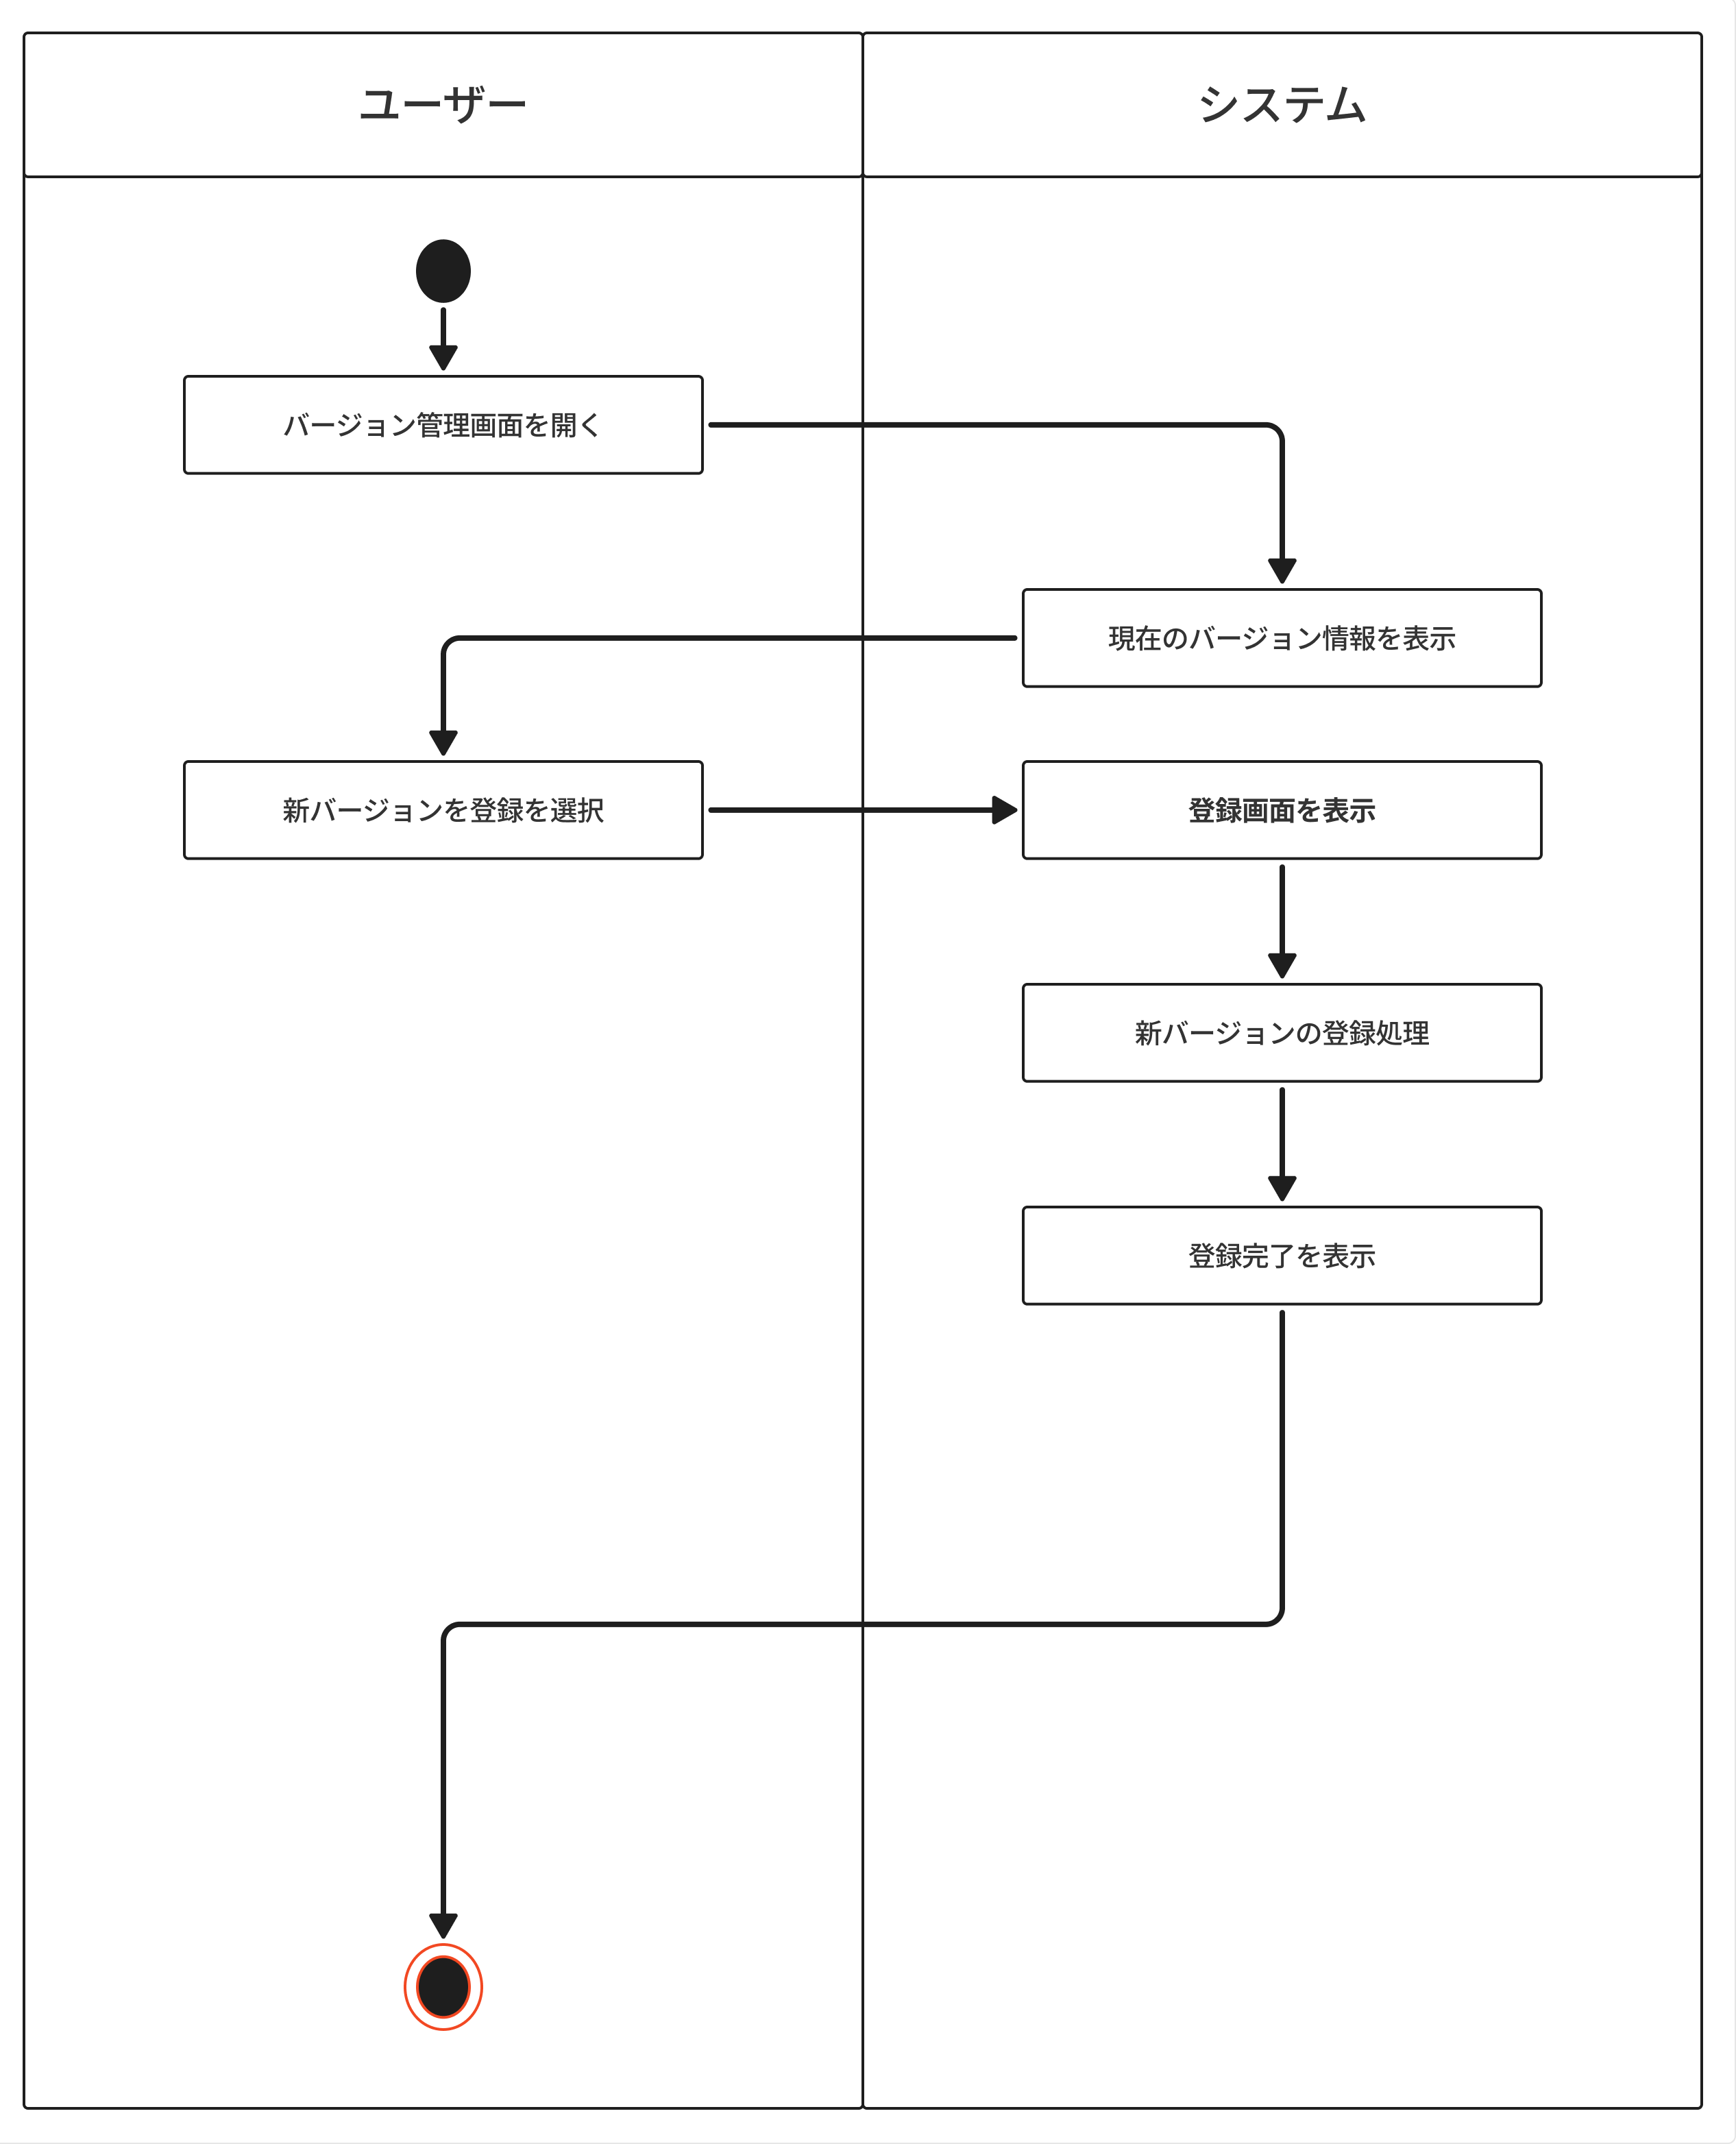
\includegraphics[width=0.5\textwidth]{chapters/images/w.png}
    \caption{お知らせ配信機能}
\end{figure}

\subsubsection{統計・ダッシュボード機能}
本機能は、アプリ全体の利用状況やアクティブユーザー数、投稿の統計データを視覚的に確認できる機能である。
\begin{figure}[H]
    \centering
    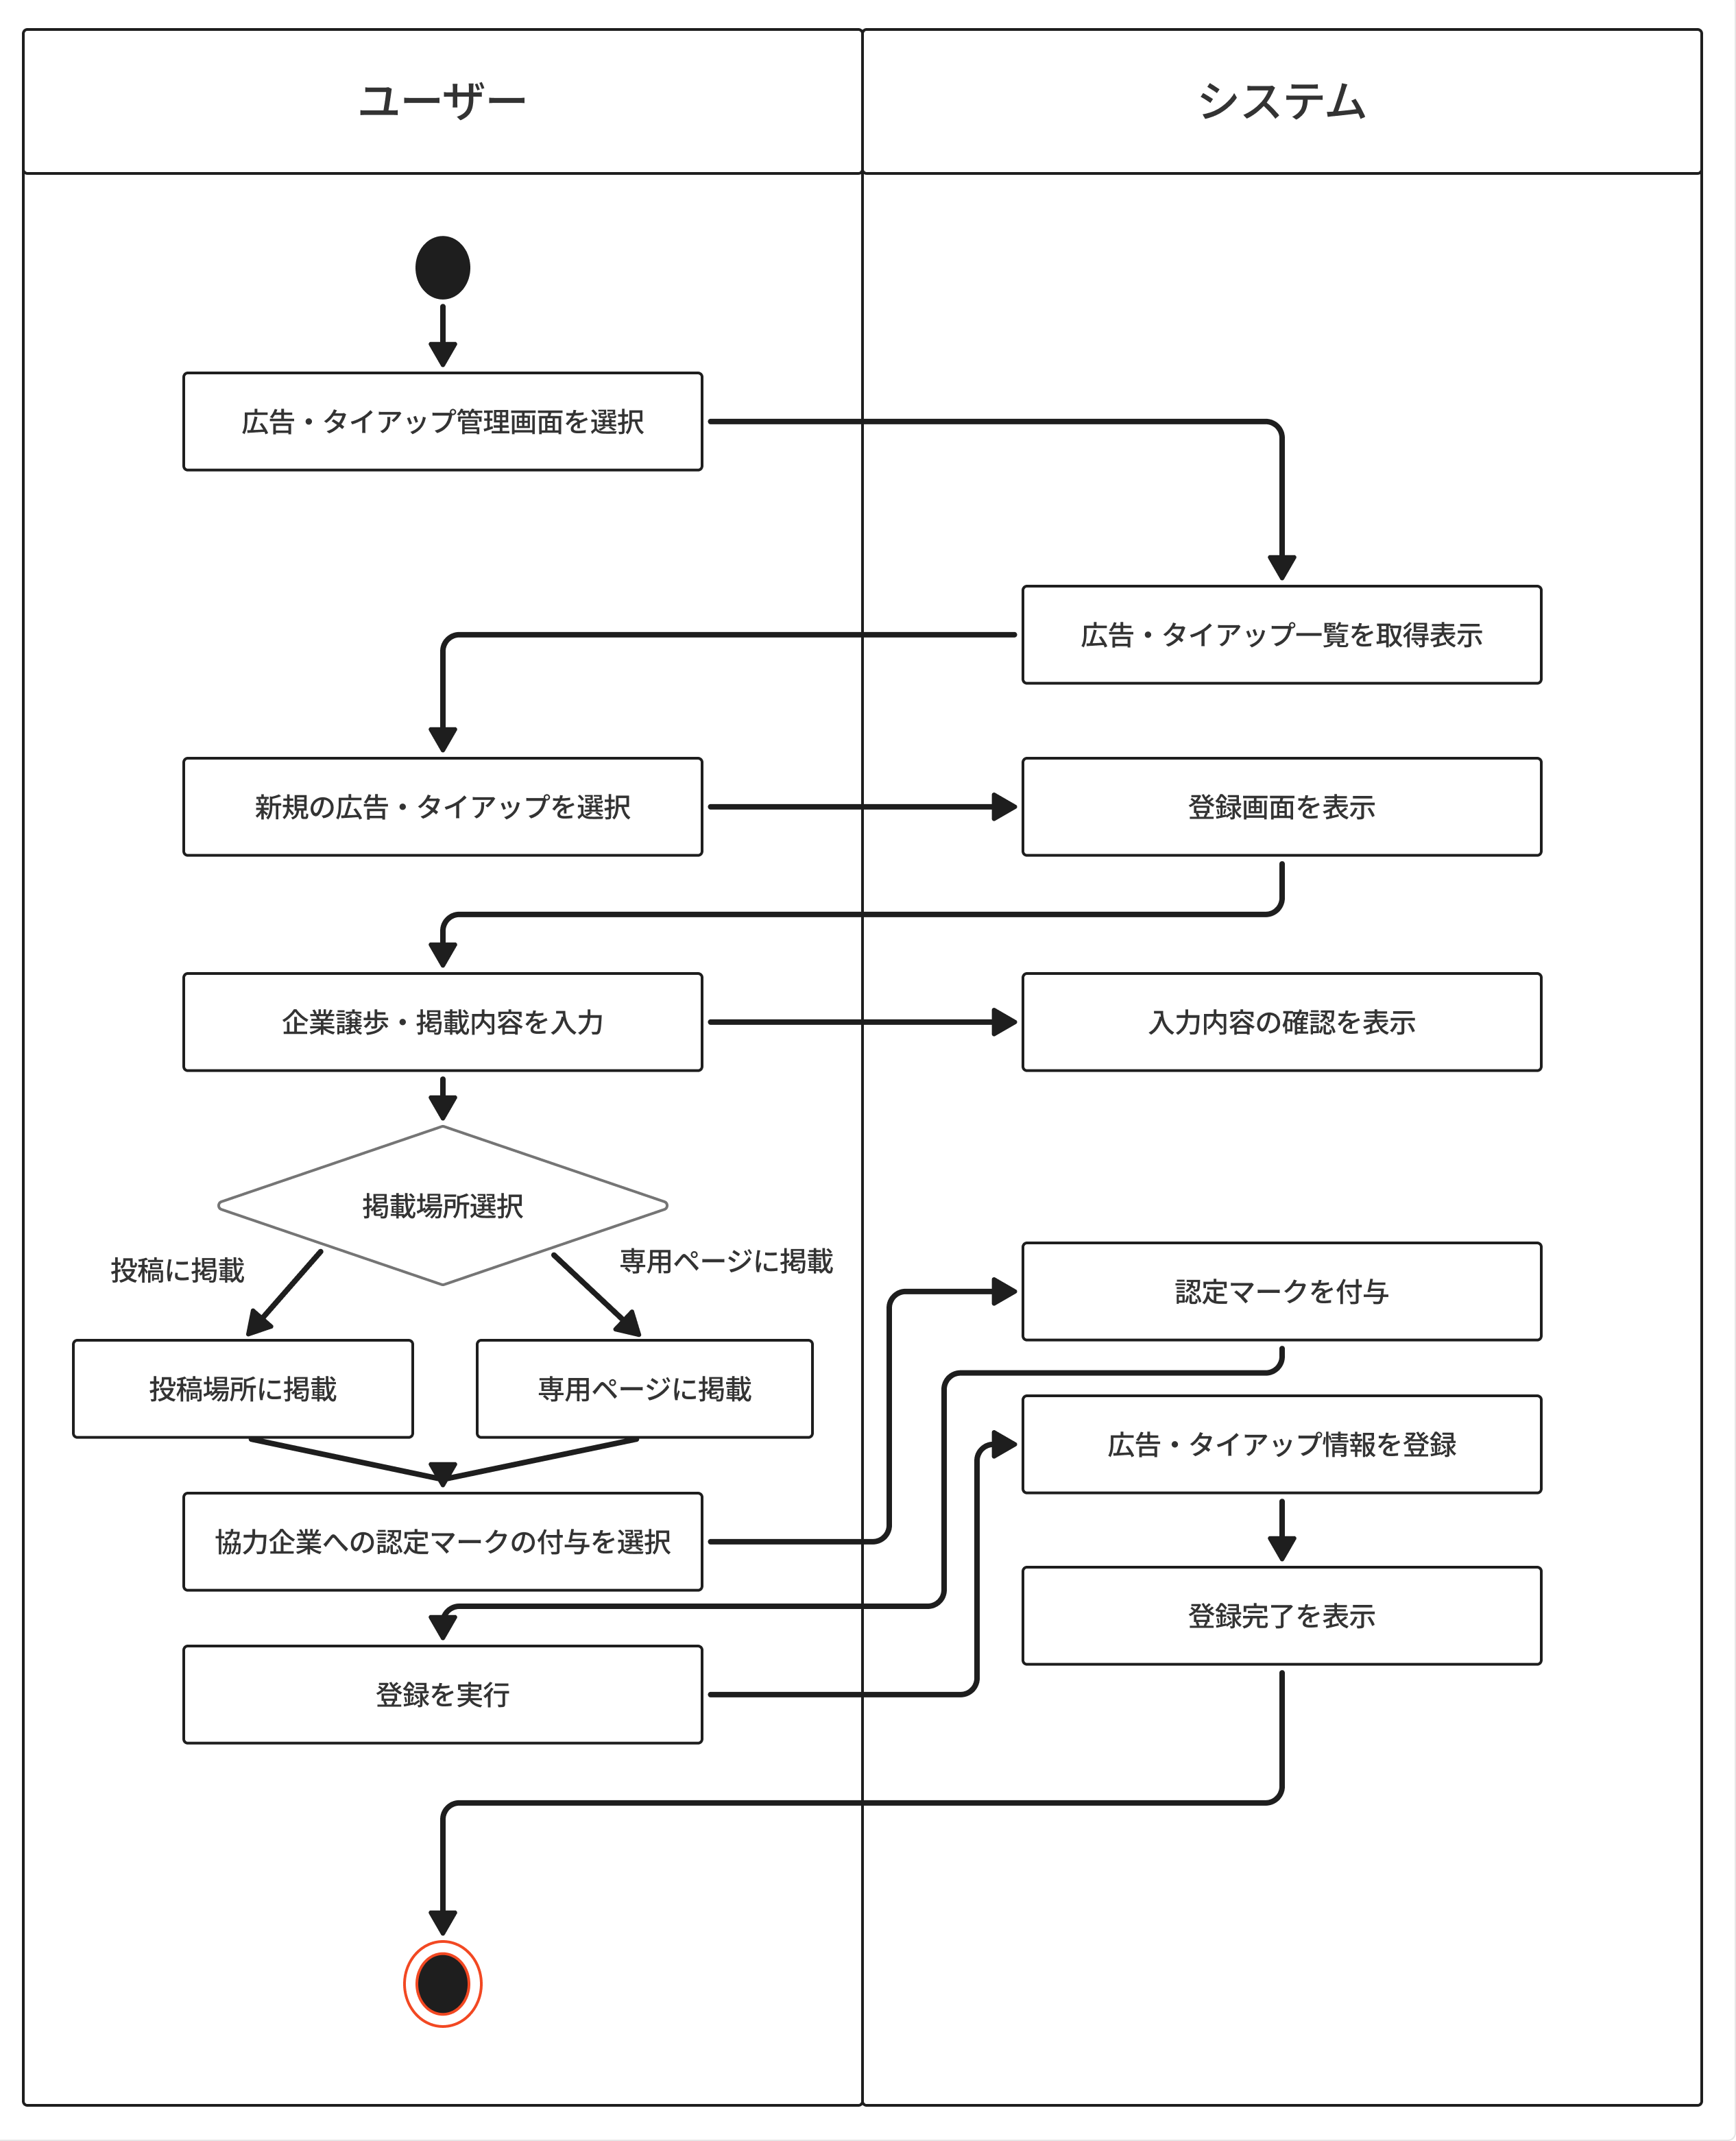
\includegraphics[width=0.5\textwidth]{chapters/images/x.png}
    \caption{統計・ダッシュボード機能}
\end{figure}

\subsubsection{ポイント・ランク設定機能}
本機能は、ユーザーに付与されるポイントの基準や、ランク・ランキングに関わる各種設定値を調整・管理する機能である。
\begin{figure}[H]
    \centering
    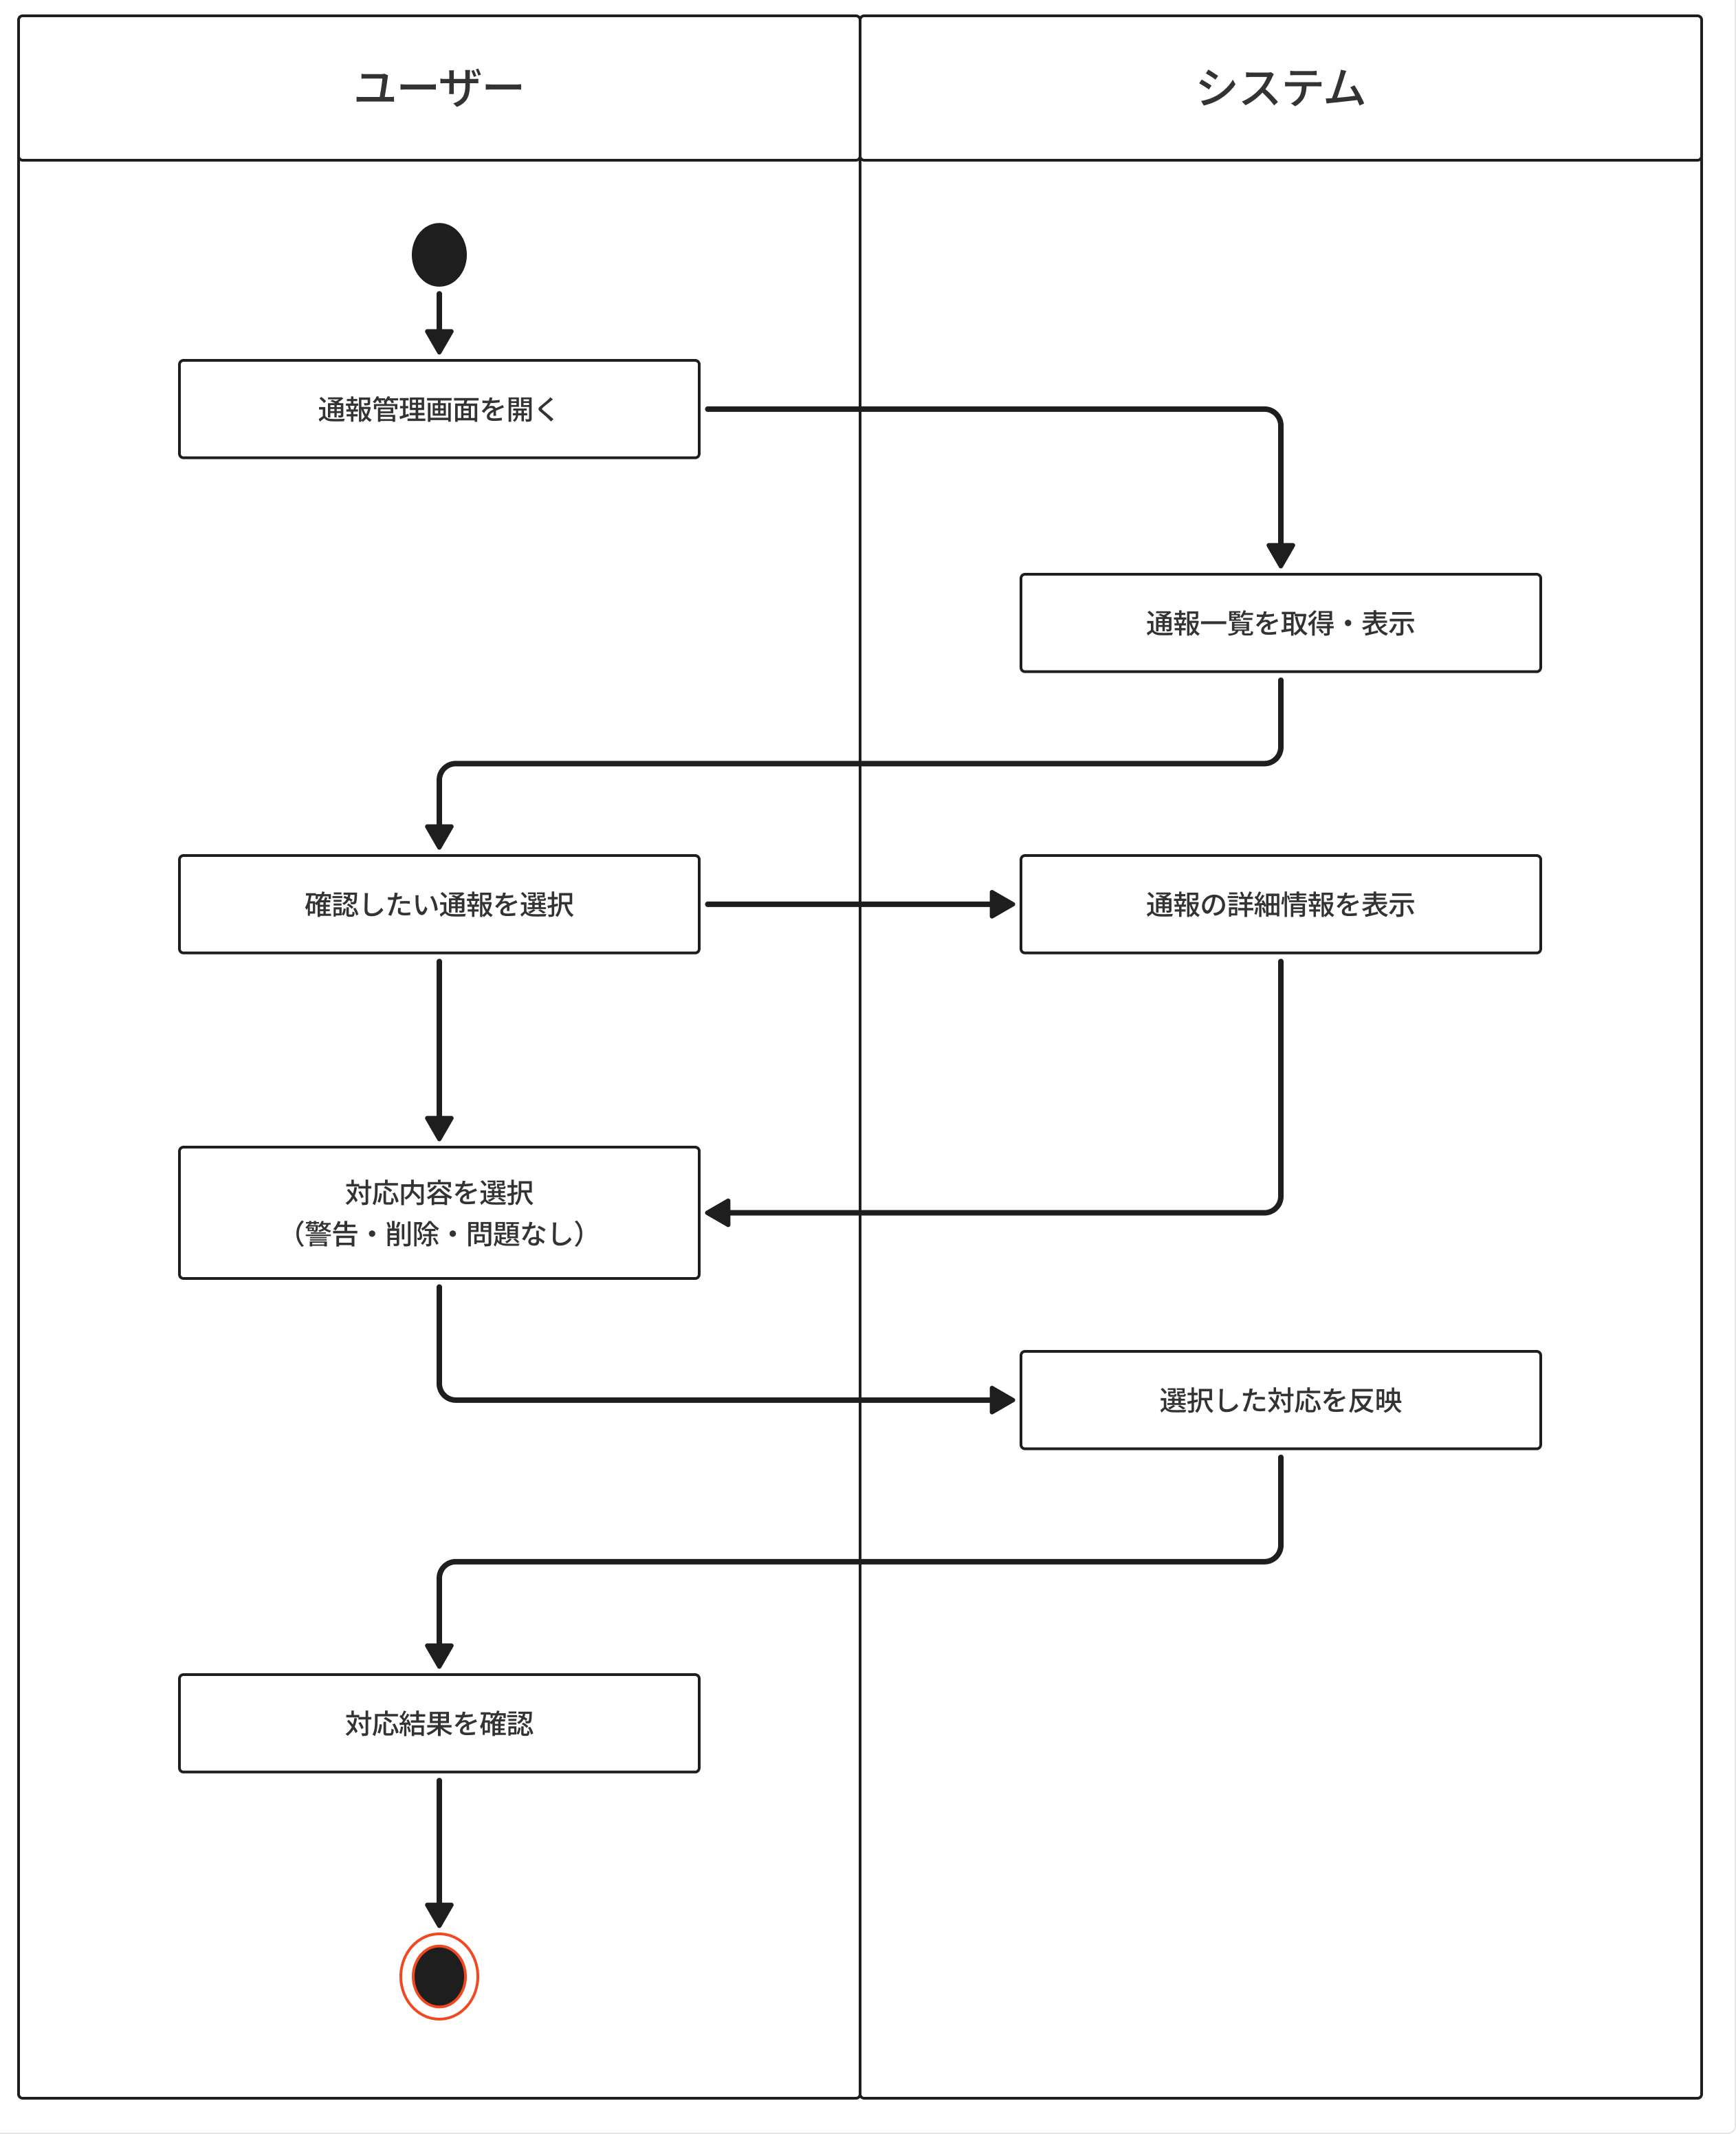
\includegraphics[width=0.5\textwidth]{chapters/images/y.png}
    \caption{ポイント・ランク設定機能}
\end{figure}

\subsubsection{システム設定機能}
本機能は、アプリケーション全体に関わる基本設定や、メンテナンスモードの切り替えなどを行う機能である。
\begin{figure}[H]
    \centering
    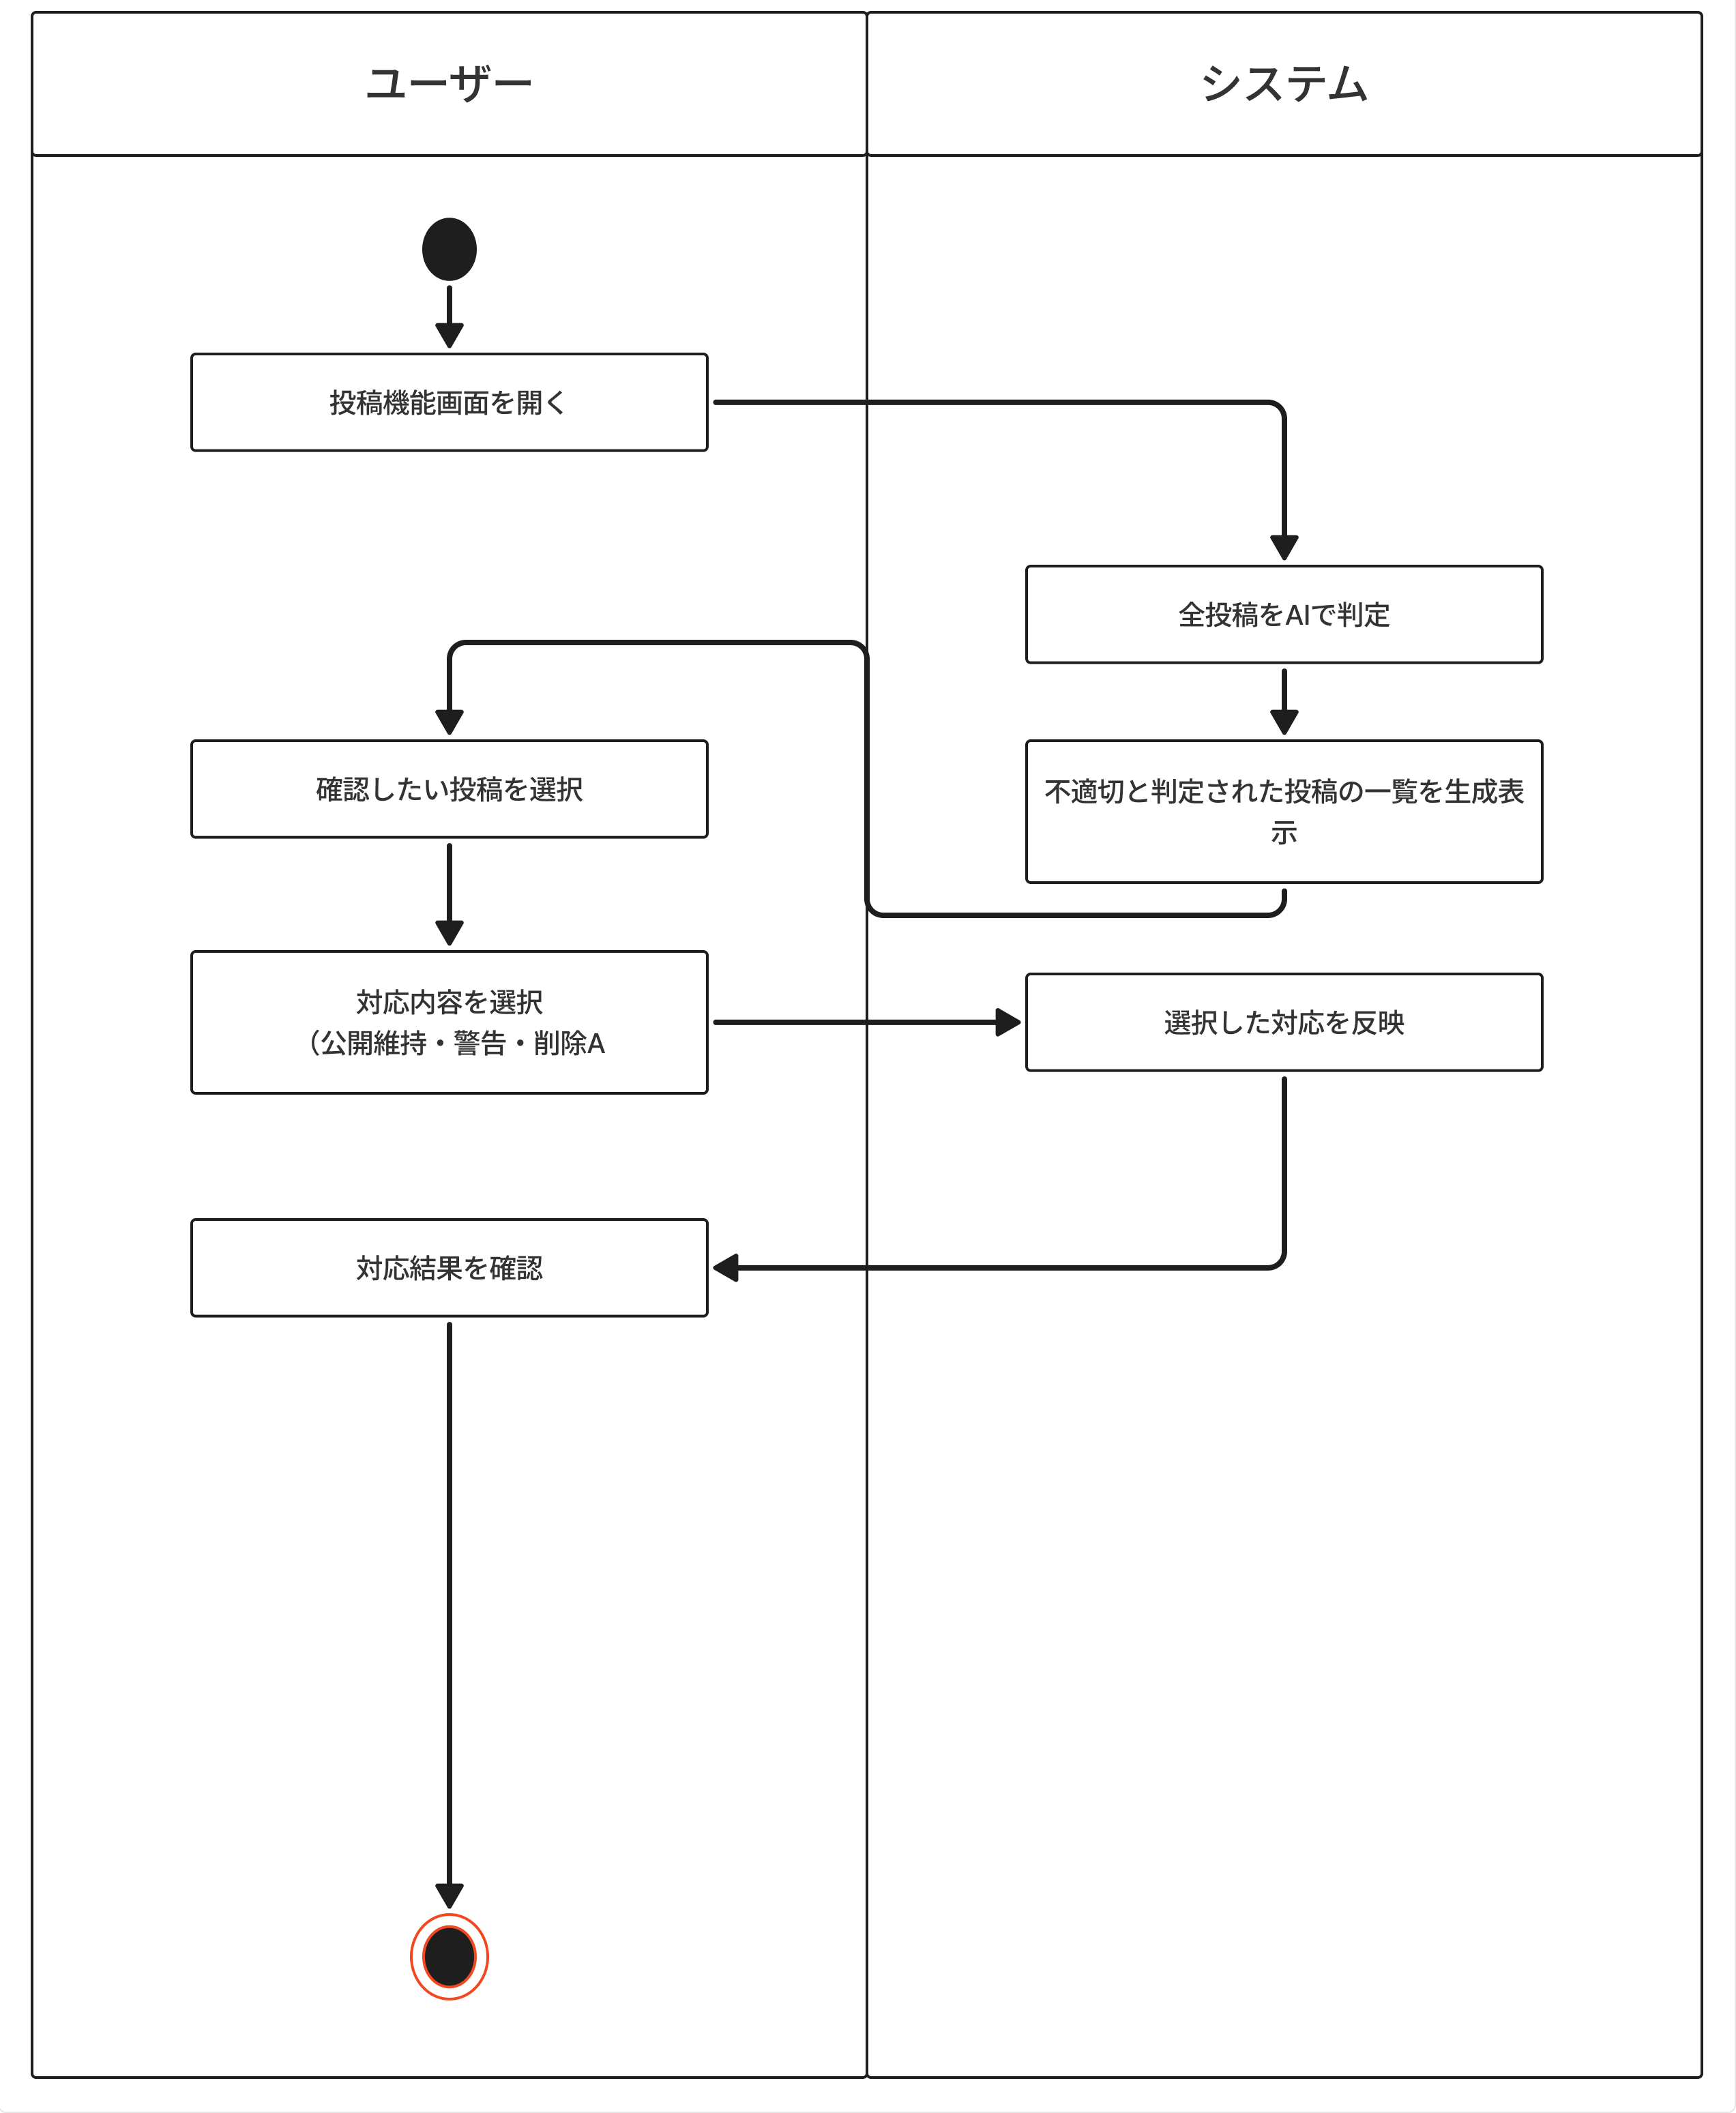
\includegraphics[width=0.5\textwidth]{chapters/images/z.png}
    \caption{システム設定機能}
\end{figure}